% Options for packages loaded elsewhere
% Options for packages loaded elsewhere
\PassOptionsToPackage{unicode,linktoc=all,pdfwindowui,pdfpagemode=FullScreen,pdfpagelayout=TwoPageRight}{hyperref}
\PassOptionsToPackage{hyphens}{url}
\PassOptionsToPackage{dvipsnames,svgnames,x11names}{xcolor}
%
\documentclass[
  9pt,
  letterpaper,
  abstract,
  titlepage]{scrbook}
\usepackage{xcolor}
\usepackage[left=1in,marginparwidth=2.0666666666667in,textwidth=4.1333333333333in,marginparsep=0.3in]{geometry}
\usepackage{amsmath,amssymb}
\setcounter{secnumdepth}{3}
\usepackage{iftex}
\ifPDFTeX
  \usepackage[T1]{fontenc}
  \usepackage[utf8]{inputenc}
  \usepackage{textcomp} % provide euro and other symbols
\else % if luatex or xetex
  \usepackage{unicode-math} % this also loads fontspec
  \defaultfontfeatures{Scale=MatchLowercase}
  \defaultfontfeatures[\rmfamily]{Ligatures=TeX,Scale=1}
\fi
\usepackage{lmodern}
\ifPDFTeX\else
  % xetex/luatex font selection
\fi
% Use upquote if available, for straight quotes in verbatim environments
\IfFileExists{upquote.sty}{\usepackage{upquote}}{}
\IfFileExists{microtype.sty}{% use microtype if available
  \usepackage[]{microtype}
  \UseMicrotypeSet[protrusion]{basicmath} % disable protrusion for tt fonts
}{}
% Make \paragraph and \subparagraph free-standing
\makeatletter
\ifx\paragraph\undefined\else
  \let\oldparagraph\paragraph
  \renewcommand{\paragraph}{
    \@ifstar
      \xxxParagraphStar
      \xxxParagraphNoStar
  }
  \newcommand{\xxxParagraphStar}[1]{\oldparagraph*{#1}\mbox{}}
  \newcommand{\xxxParagraphNoStar}[1]{\oldparagraph{#1}\mbox{}}
\fi
\ifx\subparagraph\undefined\else
  \let\oldsubparagraph\subparagraph
  \renewcommand{\subparagraph}{
    \@ifstar
      \xxxSubParagraphStar
      \xxxSubParagraphNoStar
  }
  \newcommand{\xxxSubParagraphStar}[1]{\oldsubparagraph*{#1}\mbox{}}
  \newcommand{\xxxSubParagraphNoStar}[1]{\oldsubparagraph{#1}\mbox{}}
\fi
\makeatother


\providecommand{\tightlist}{%
  \setlength{\itemsep}{0pt}\setlength{\parskip}{0pt}}\usepackage{longtable,booktabs,array}
\usepackage{multirow}
\usepackage{calc} % for calculating minipage widths
% Correct order of tables after \paragraph or \subparagraph
\usepackage{etoolbox}
\makeatletter
\patchcmd\longtable{\par}{\if@noskipsec\mbox{}\fi\par}{}{}
\makeatother
% Allow footnotes in longtable head/foot
\IfFileExists{footnotehyper.sty}{\usepackage{footnotehyper}}{\usepackage{footnote}}
\makesavenoteenv{longtable}
\usepackage{graphicx}
\makeatletter
\newsavebox\pandoc@box
\newcommand*\pandocbounded[1]{% scales image to fit in text height/width
  \sbox\pandoc@box{#1}%
  \Gscale@div\@tempa{\textheight}{\dimexpr\ht\pandoc@box+\dp\pandoc@box\relax}%
  \Gscale@div\@tempb{\linewidth}{\wd\pandoc@box}%
  \ifdim\@tempb\p@<\@tempa\p@\let\@tempa\@tempb\fi% select the smaller of both
  \ifdim\@tempa\p@<\p@\scalebox{\@tempa}{\usebox\pandoc@box}%
  \else\usebox{\pandoc@box}%
  \fi%
}
% Set default figure placement to htbp
\def\fps@figure{htbp}
\makeatother
% definitions for citeproc citations
\NewDocumentCommand\citeproctext{}{}
\NewDocumentCommand\citeproc{mm}{%
  \begingroup\def\citeproctext{#2}\cite{#1}\endgroup}
\makeatletter
 % allow citations to break across lines
 \let\@cite@ofmt\@firstofone
 % avoid brackets around text for \cite:
 \def\@biblabel#1{}
 \def\@cite#1#2{{#1\if@tempswa , #2\fi}}
\makeatother
\newlength{\cslhangindent}
\setlength{\cslhangindent}{1.5em}
\newlength{\csllabelwidth}
\setlength{\csllabelwidth}{3em}
\newenvironment{CSLReferences}[2] % #1 hanging-indent, #2 entry-spacing
 {\begin{list}{}{%
  \setlength{\itemindent}{0pt}
  \setlength{\leftmargin}{0pt}
  \setlength{\parsep}{0pt}
  % turn on hanging indent if param 1 is 1
  \ifodd #1
   \setlength{\leftmargin}{\cslhangindent}
   \setlength{\itemindent}{-1\cslhangindent}
  \fi
  % set entry spacing
  \setlength{\itemsep}{#2\baselineskip}}}
 {\end{list}}
\usepackage{calc}
\newcommand{\CSLBlock}[1]{\hfill\break\parbox[t]{\linewidth}{\strut\ignorespaces#1\strut}}
\newcommand{\CSLLeftMargin}[1]{\parbox[t]{\csllabelwidth}{\strut#1\strut}}
\newcommand{\CSLRightInline}[1]{\parbox[t]{\linewidth - \csllabelwidth}{\strut#1\strut}}
\newcommand{\CSLIndent}[1]{\hspace{\cslhangindent}#1}

% =============================================================================
% LATEX HEADER CONFIGURATION FOR MLSYSBOOK PDF
% =============================================================================
% This file contains all LaTeX package imports, custom commands, and styling
% definitions for the PDF output of the Machine Learning Systems textbook.
%
% Key Features:
% - Harvard crimson branding throughout
% - Custom part/chapter/section styling
% - Professional table formatting with colored headers
% - Margin notes with custom styling
% - TikZ-based part dividers
% - Page numbering (Roman for frontmatter, Arabic for mainmatter)
%
% Note: This file is included via _quarto-pdf.yml and affects PDF output only.
% HTML/EPUB styling is handled separately via CSS files.
% =============================================================================

% =============================================================================
% PACKAGE IMPORTS
% =============================================================================

% Layout and positioning
% \usepackage[outercaption, ragged]{sidecap}  % Commented out to make figure captions inline instead of in margin
\usepackage{adjustbox}      % Adjusting box dimensions
\usepackage{afterpage}      % Execute commands after page break
\usepackage{morefloats}     % Increase number of floats
\usepackage{array}          % Enhanced table column formatting
\usepackage{atbegshi}       % Insert content at page beginning
%\usepackage{changepage}     % Change page dimensions mid-document
\usepackage{emptypage}      % Clear headers/footers on empty pages

% Language and text
\usepackage[english]{babel} % English language support
\usepackage{microtype}      % Improved typography and hyphenation

% Captions and floats
\usepackage{caption}
% Caption styling configuration
%\captionsetup[table]{belowskip=5pt}
\captionsetup{format=plain}
\DeclareCaptionLabelFormat{mylabel}{#1
#2:\hspace{1.0ex}}
\DeclareCaptionFont{ninept}{\fontsize{7pt}{8}\selectfont #1}

% Figure captions: Small font, bold label, ragged right
\captionsetup[figure]{labelfont={bf,ninept},labelsep=space,
belowskip=2pt,aboveskip=6pt,labelformat=mylabel,
justification=raggedright,singlelinecheck=false,font={ninept}}

% Table captions: Small font, bold label, ragged right
\captionsetup[table]{belowskip=6pt,labelfont={bf,ninept},labelsep=none,
labelformat=mylabel,justification=raggedright,singlelinecheck=false,font={ninept}}

% Typography fine-tuning
\emergencystretch=5pt       % Allow extra stretch to avoid overfull boxes

% Utility packages
\usepackage{etoolbox}       % For patching commands and environments

% Page layout and headers
\usepackage{fancyhdr}       % Custom headers and footers
\usepackage{geometry}       % Page dimensions and margins

% Graphics and figures
\usepackage{graphicx}       % Include graphics
\usepackage{float}          % Improved float placement
\usepackage[skins,breakable]{tcolorbox} % Coloured and framed text boxes
\tcbset{before upper=\setlength{\parskip}{3pt}}

% Tables
\usepackage{longtable}      % Multi-page tables

% Fonts and typography
\usepackage{fontspec}       % Font selection for LuaLaTeX
\usepackage{mathptmx}       % Times-like math fonts
\usepackage{newpxtext}      % Palatino-like font for body text

% Colors and visual elements
\usepackage[dvipsnames]{xcolor}  % Extended color support
\usepackage{tikz}           % Programmatic graphics
\usetikzlibrary{positioning}
\usetikzlibrary{calc}
\usepackage{tikzpagenodes}  % TikZ positioning relative to page

% Code listings
\usepackage{listings}       % Code highlighting

% Hyperlinks
\usepackage{hyperref}       % Clickable links in PDF

% Conditional logic
\usepackage{ifthen}         % If-then-else commands

% Math symbols
\usepackage{amsmath}        % AMS math extensions
\usepackage{amssymb}        % AMS math symbols
\usepackage{latexsym}       % Additional LaTeX symbols
\usepackage{pifont}         % Zapf Dingbats symbols
\providecommand{\blacklozenge}{\ding{117}}  % Black diamond symbol

% Lists
\usepackage{enumitem}       % Customizable lists

% Margin notes and sidenotes
\usepackage{marginfix}      % Fixes margin note overflow
\usepackage{marginnote}     % Margin notes
\usepackage{sidenotes}      % Academic-style sidenotes
\renewcommand\raggedrightmarginnote{\sloppy}
\renewcommand\raggedleftmarginnote{\sloppy}

% Typography improvements
\usepackage{ragged2e}       % Better ragged text
\usepackage[all]{nowidow}   % Prevent widows and orphans
\usepackage{needspace}      % Ensure minimum space on page

% Section formatting
\usepackage[explicit]{titlesec}  % Custom section titles
\usepackage{tocloft}        % Table of contents formatting

% QR codes and icons
\usepackage{fontawesome5}   % Font Awesome icons
\usepackage{qrcode}         % QR code generation
\qrset{link, height=15mm}

% =============================================================================
% FLOAT CONFIGURATION
% =============================================================================
% Allow more floats per page to handle figure-heavy chapters
\extrafloats{200}
\setcounter{topnumber}{12}       % Max floats at top of page
\setcounter{bottomnumber}{12}    % Max floats at bottom of page
\setcounter{totalnumber}{24}     % Max floats per page
\setcounter{dbltopnumber}{8}     % Max floats at top of two-column page
\renewcommand{\topfraction}{.95}  % Max fraction of page for top floats
\renewcommand{\bottomfraction}{.95}
\renewcommand{\textfraction}{.05}  % Min fraction of page for text
\renewcommand{\floatpagefraction}{.7}  % Min fraction of float page
\renewcommand{\dbltopfraction}{.95}

% Prevent "Float(s) lost" errors by flushing floats more aggressively
\usepackage{placeins}  % Provides \FloatBarrier

% =============================================================================
% COLOR DEFINITIONS
% =============================================================================
% Harvard crimson - primary brand color used throughout
\definecolor{crimson}{HTML}{A51C30}

% Quiz element colors
\definecolor{quiz-question-color1}{RGB}{225,243,248}  % Light blue background
\definecolor{quiz-question-color2}{RGB}{17,158,199}   % Blue border
\definecolor{quiz-answer-color1}{RGB}{250,234,241}    % Light pink background
\definecolor{quiz-answer-color2}{RGB}{152,14,90}      % Magenta border

% =============================================================================
% LIST FORMATTING
% =============================================================================
% Tighter list spacing for academic style
\def\tightlist{}
\setlist{itemsep=1pt, parsep=1pt, topsep=0pt,after={\vspace{0.3\baselineskip}}}
\let\tightlist\relax

\makeatletter
\@ifpackageloaded{framed}{}{\usepackage{framed}}
\@ifpackageloaded{fancyvrb}{}{\usepackage{fancyvrb}}
\makeatother

\makeatletter
%New float "codelisting" has been updated
\AtBeginDocument{%
\floatstyle{ruled}
\newfloat{codelisting}{!htb}{lop}
\floatname{codelisting}{Listing}
\floatplacement{codelisting}{!htb}
\captionsetup[codelisting]{labelfont={bf,ninept},labelformat=mylabel,
  singlelinecheck=false,width=\linewidth,labelsep=none,font={ninept}}%
\renewenvironment{snugshade}{%
   \def\OuterFrameSep{3pt}%
   \def\FrameCommand{\fboxsep=5pt\colorbox{shadecolor}}%
   \MakeFramed{\advance\hsize-\width\FrameRestore}%
   \leftskip 0.5em \rightskip 0.5em%
   \small% decrease font size
   }{\endMakeFramed}%
}
\makeatother

%The space before and after the verbatim environment "Highlighting" has been reduced
\fvset{listparameters=\setlength{\topsep}{0pt}\setlength{\partopsep}{0pt}}
\DefineVerbatimEnvironment{Highlighting}{Verbatim}{framesep=0mm,commandchars=\\\{\}}

\makeatletter
\renewcommand\fs@ruled{\def\@fs@cfont{\bfseries}\let\@fs@capt\floatc@ruled
\def\@fs@pre{\hrule height.8pt depth0pt \kern2pt}%
\def\@fs@post{\kern2pt\hrule\relax}%
\def\@fs@mid{\kern2pt\hrule\kern1pt}%space between float and caption
\let\@fs@iftopcapt\iftrue}
\makeatother


% =============================================================================
% HYPHENATION RULES
% =============================================================================
% Explicit hyphenation points for technical terms to avoid bad breaks
\hyphenation{
  light-weight
  light-weight-ed
  de-vel-op-ment
  un-der-stand-ing
  mod-els
  prin-ci-ples
  ex-per-tise
  com-pli-cat-ed
  blue-print
  per‧for‧mance
  com-mu-ni-ca-tion
  par-a-digms
  hy-per-ten-sion
  a-chieved
}

% =============================================================================
% CODE LISTING CONFIGURATION
% =============================================================================
% Settings for code blocks using listings package
\lstset{
breaklines=true,              % Automatic line wrapping
breakatwhitespace=true,       % Break at whitespace only
basicstyle=\ttfamily,         % Monospace font
frame=none,                   % No frame around code
keepspaces=true,              % Preserve spaces
showspaces=false,             % Don't show space characters
showtabs=false,               % Don't show tab characters
columns=flexible,             % Flexible column width
belowskip=0pt,               % Minimal spacing
aboveskip=0pt
}

% =============================================================================
% PAGE GEOMETRY
% =============================================================================
% MIT Press trim size: 7" x 10" (per publisher specifications)
% This is a standard academic textbook format providing good readability
% for technical content with figures and code blocks.
% Wide outer margin accommodates sidenotes/margin notes.
\geometry{
  paperwidth=7in,
  paperheight=10in,
  top=0.875in,
  bottom=0.875in,
  inner=0.875in,              % Inner margin (binding side)
  outer=1.75in,               % Outer margin (includes space for sidenotes)
  footskip=30pt,
  marginparwidth=1.25in,      % Width for margin notes
  twoside                     % Different left/right pages
}

% =============================================================================
% SIDENOTE STYLING
% =============================================================================
% Custom sidenote design with crimson vertical bar
\renewcommand{\thefootnote}{\textcolor{crimson}{\arabic{footnote}}}

% Save original sidenote command
\makeatletter
\@ifundefined{oldsidenote}{
  \let\oldsidenote\sidenote%
}{}
\makeatother

% Redefine sidenote with vertical crimson bar
\renewcommand{\sidenote}[1]{%
  \oldsidenote{%
    \noindent
    \color{crimson!100}                        % Crimson vertical line
    \raisebox{0em}{%
      \rule{0.5pt}{1.5em}                      % Thin vertical line
    }
    \hspace{0.3em}                             % Space after line
    \color{black}                              % Reset text color
    \footnotesize #1                           % Sidenote content
  }%
}

% =============================================================================
% FLOAT HANDLING
% =============================================================================
% Patch LaTeX's output routine to handle float overflow gracefully
% The "Float(s) lost" error occurs in \@doclearpage when \@currlist is not empty
% This patch silently clears pending floats that can't be placed
\makeatletter
\let\orig@doclearpage\@doclearpage
\def\@doclearpage{%
  \ifx\@currlist\@empty\else
    \global\let\@currlist\@empty
    \typeout{Warning: Floats cleared to prevent overflow}%
  \fi
  \orig@doclearpage
}
\makeatother

% Additional safety for structural commands
\let\originalbackmatter\backmatter
\renewcommand{\backmatter}{%
  \clearpage%
  \originalbackmatter%
}

\let\originalfrontmatter\frontmatter
\renewcommand{\frontmatter}{%
  \clearpage%
  \originalfrontmatter%
}

\let\originalmainmatter\mainmatter
\renewcommand{\mainmatter}{%
  \clearpage%
  \originalmainmatter%
}

% =============================================================================
% PAGE HEADERS AND FOOTERS
% =============================================================================
% Ensure chapters use fancy page style (not plain)
\patchcmd{\chapter}{\thispagestyle{plain}}{\thispagestyle{fancy}}{}{}

% Main page style with crimson headers
\pagestyle{fancy}
\fancyhf{}                                              % Clear all
\fancyhead[LE]{\small\color{crimson}\nouppercase{\rightmark}}  % Left even: section
\fancyhead[RO]{\color{crimson}\thepage}                 % Right odd: page number
\fancyhead[LO]{\small\color{crimson}\nouppercase{\leftmark}}   % Left odd: chapter
\fancyhead[RE]{\color{crimson}\thepage}                 % Right even: page number
\renewcommand{\headrulewidth}{0.4pt}                    % Thin header line
\renewcommand{\footrulewidth}{0pt}                      % No footer line

% Plain page style (for chapter openings)
\fancypagestyle{plain}{
  \fancyhf{}
  \fancyfoot[C]{\color{crimson}\thepage}                % Centered page number
  \renewcommand{\headrulewidth}{0pt}
  \renewcommand{\footrulewidth}{0pt}
}

% =============================================================================
% KOMA-SCRIPT FONT ADJUSTMENTS
% =============================================================================
% Apply crimson color to all heading levels
\addtokomafont{disposition}{\rmfamily\color{crimson}}
\addtokomafont{chapter}{\color{crimson}}
\addtokomafont{section}{\color{crimson}}
\addtokomafont{subsection}{\color{crimson}}

% =============================================================================
% ABSTRACT ENVIRONMENT
% =============================================================================
\newenvironment{abstract}{
  \chapter*{\abstractname}
  \addcontentsline{toc}{chapter}{\abstractname}
  \small
}{
  \clearpage
}

% =============================================================================
% HYPERLINK CONFIGURATION
% =============================================================================
% Crimson-colored links throughout, two-page PDF layout
\hypersetup{
  linkcolor=crimson,
  citecolor=crimson,
  urlcolor=crimson,
  pdfpagelayout=TwoPageRight,   % Two-page spread view
  pdfstartview=Fit               % Initial zoom fits page
}

% =============================================================================
% PART SUMMARY SYSTEM
% =============================================================================
% Allows adding descriptive text below part titles
\newcommand{\partsummary}{}     % Empty by default
\newif\ifhaspartsummary%
\haspartsummaryfalse%

\newcommand{\setpartsummary}[1]{%
  \renewcommand{\partsummary}{#1}%
  \haspartsummarytrue%
}

% Additional colors for part page backgrounds
\definecolor{BrownLL}{RGB}{233,222,220}
\definecolor{BlueDD}{RGB}{62,100,125}
\colorlet{BlueDD}{magenta}

% ===============================================================================
% PART STYLING SYSTEM
% ===============================================================================
%
% This system provides three distinct visual styles for book organization:
%
% 1. NUMBERED PARTS (\part{title}) - For main book sections
%    - Roman numerals (I, II, III, etc.) in top right corner
%    - Crimson title with horizontal lines above/below
%    - "Part I" label in sidebar
%    - Used for: foundations, principles, optimization, deployment, etc.
%
% 2. UNNUMBERED PARTS (\part*{title}) - For special sections like "Labs"
%    - Division-style geometric background (left side)
%    - No Roman numerals
%    - Used for: labs section
%
% 3. DIVISIONS (\division{title}) - For major book divisions
%    - Clean geometric background with centered title
%    - Used for: frontmatter, main_content, backmatter
%
% The Lua filter (inject-parts.lua) automatically routes parts by {key:xxx} commands
% to the appropriate LaTeX command based on the key name.
% ===============================================================================

% NUMBERED PARTS: Roman numeral styling for main book sections
\titleformat{\part}[display]
{\thispagestyle{empty}}{}{20pt}{
\begin{tikzpicture}[remember picture,overlay]
%%%
%%
\node[crimson,align=flush right,
inner sep=0,outer sep=0mm,draw=none,%
anchor=east,minimum height=31mm, text width=1.2\textwidth,
yshift=-30mm,font={%
\fontsize{98pt}{104}\selectfont\bfseries}]  (BG) at (current page text area.north east){\thepart};
%
\node[black,inner sep=0mm,draw=none,
anchor=mid,text width=1.2\textwidth,
 minimum height=35mm, align=right,
node distance=7mm,below=of BG,
font={\fontsize{30pt}{34}\selectfont}]
(BGG)  {\hyphenchar\font=-1 \color{black}\MakeUppercase {#1}};
\draw [crimson,line width=3pt] ([yshift=0mm]BGG.north west) -- ([yshift=0mm]BGG.north east);
\draw [crimson,line width=2pt] ([yshift=0mm]BGG.south west) -- ([yshift=0mm]BGG.south east);
%
\node[fill=crimson,text=white,rotate=90,%
anchor=south west,minimum height=15mm,
minimum width=40mm,font={%
\fontsize{20pt}{20}\selectfont\bfseries}](BP)  at
(current page text area.south east)
{{\sffamily Part}~\thepart};
%
\path[red](BP.north west)-|coordinate(PS)(BGG.south west);
%
% Part summary box commented out for cleaner design
% \ifhaspartsummary
% \node[inner sep=4pt,text width=0.7\textwidth,draw=none,fill=BrownLL!40,
% align=justify,font={\fontsize{9pt}{12}\selectfont},anchor=south west]
% at (PS) {\partsummary};
% \fi
\end{tikzpicture}
}[]

\renewcommand{\thepart}{\Roman{part}}

% UNNUMBERED PARTS: Division-style background for special sections
\titleformat{name=\part,numberless}[display]
{\thispagestyle{empty}}{}{20pt}{
\begin{tikzpicture}[remember picture,overlay]
%%%
\coordinate(S1)at([yshift=-200mm]current page.north west);
\draw[draw=none,fill=BlueDD!7](S1)--++(45:16)coordinate(S2)-
|(S2|-current page.north west)--(current page.north west)coordinate(S3)--(S1);
%
\coordinate(E1)at([yshift=-98mm]current page.north west);
\draw[draw=none,fill=BlueDD!15](E1)--(current page.north west)coordinate(E2)
--++(0:98mm)coordinate(E3)--(E1);
%
\coordinate(D1)at([yshift=15mm]current page.south west);
\draw[draw=none,fill=BlueDD!40,opacity=0.5](D1)--++(45:5.5)coordinate(D2)
-|(D2|-current page.north west)--(current page.north west)coordinate(D3)--(D1);
%%%%
\path[red](S2)-|(S2-|current page.east)coordinate(SS2);
%PART
\node[crimson,align=flush right,inner sep=0,outer sep=0mm,draw=none,anchor=south,
font={\fontsize{48pt}{48}\selectfont\bfseries}]  (BG) at ($(S2)!0.5!(SS2)$){\hphantom{Part}};
%%%
\path[green]([yshift=15mm]D2)-|coordinate(TPD)(BG.south east);
\node[inner sep=0mm,draw=none,anchor=south east,%text width=0.9\textwidth,
align=right,font={\fontsize{40pt}{40}\selectfont}]
(BGG) at (TPD)  {\color{crimson}\MakeUppercase {#1}};%\MakeUppercase {}
\end{tikzpicture}
}

% Define \numberedpart command for numbered parts
\newcommand{\numberedpart}[1]{%
\FloatBarrier%  % Flush all pending floats before part break
\clearpage
\thispagestyle{empty}
\stepcounter{part}%
\begin{tikzpicture}[remember picture,overlay]
%%%
%%
\node[crimson,align=flush right,
inner sep=0,outer sep=0mm,draw=none,%
anchor=east,minimum height=31mm, text width=1.2\textwidth,
yshift=-30mm,font={%
\fontsize{98pt}{104}\selectfont\bfseries}]  (BG) at (current page text area.north east){\thepart};
%
\node[black,inner sep=0mm,draw=none,
anchor=mid,text width=1.2\textwidth,
 minimum height=35mm, align=right,
node distance=7mm,below=of BG,
font={\fontsize{30pt}{34}\selectfont}]
(BGG)  {\hyphenchar\font=-1 \color{black}\MakeUppercase {#1}};
\draw [crimson,line width=3pt] ([yshift=0mm]BGG.north west) -- ([yshift=0mm]BGG.north east);
\draw [crimson,line width=2pt] ([yshift=0mm]BGG.south west) -- ([yshift=0mm]BGG.south east);
%
\node[fill=crimson,text=white,rotate=90,%
anchor=south west,minimum height=15mm,
minimum width=40mm,font={%
\fontsize{20pt}{20}\selectfont\bfseries}](BP)  at
(current page text area.south east)
{{\sffamily Part}~\thepart};
%
\path[red](BP.north west)-|coordinate(PS)(BGG.south west);
%
% Part summary box commented out for cleaner design
% \ifhaspartsummary
% \node[inner sep=4pt,text width=0.7\textwidth,draw=none,fill=BrownLL!40,
% align=justify,font={\fontsize{9pt}{12}\selectfont},anchor=south west]
% at (PS) {\partsummary};
% \fi
\end{tikzpicture}
\clearpage
}



% DIVISIONS: Clean geometric styling with subtle tech elements
% Used for frontmatter, main_content, and backmatter divisions
\newcommand{\division}[1]{%
\FloatBarrier%  % Flush all pending floats before division break
\clearpage
\thispagestyle{empty}
\begin{tikzpicture}[remember picture,overlay]

% Clean geometric background (original design)
\coordinate(S1)at([yshift=-200mm]current page.north west);
\draw[draw=none,fill=BlueDD!7](S1)--++(45:16)coordinate(S2)-
|(S2|-current page.north west)--(current page.north west)coordinate(S3)--(S1);

\coordinate(E1)at([yshift=-98mm]current page.north west);
\draw[draw=none,fill=BlueDD!15](E1)--(current page.north west)coordinate(E2)
--++(0:98mm)coordinate(E3)--(E1);

\coordinate(D1)at([yshift=15mm]current page.south west);
\draw[draw=none,fill=BlueDD!40,opacity=0.5](D1)--++(45:5.5)coordinate(D2)
-|(D2|-current page.north west)--(current page.north west)coordinate(D3)--(D1);

% Subtle tech elements - positioned in white areas for better visibility
% Upper right white area - more visible
\draw[crimson!40, line width=0.8pt] ([xshift=140mm,yshift=-60mm]current page.north west) -- ++(40mm,0);
\draw[crimson!40, line width=0.8pt] ([xshift=150mm,yshift=-70mm]current page.north west) -- ++(30mm,0);
\draw[crimson!35, line width=0.7pt] ([xshift=160mm,yshift=-60mm]current page.north west) -- ++(0,-15mm);
\draw[crimson!35, line width=0.7pt] ([xshift=170mm,yshift=-70mm]current page.north west) -- ++(0,10mm);

% Circuit nodes - upper right
\fill[crimson!50] ([xshift=160mm,yshift=-60mm]current page.north west) circle (1.5mm);
\fill[white] ([xshift=160mm,yshift=-60mm]current page.north west) circle (0.8mm);
\fill[crimson!50] ([xshift=170mm,yshift=-70mm]current page.north west) circle (1.3mm);
\fill[white] ([xshift=170mm,yshift=-70mm]current page.north west) circle (0.6mm);

% Lower right white area - enhanced visibility
\draw[crimson!45, line width=0.9pt] ([xshift=140mm,yshift=-190mm]current page.north west) -- ++(45mm,0);
\draw[crimson!45, line width=0.9pt] ([xshift=150mm,yshift=-200mm]current page.north west) -- ++(35mm,0);
\draw[crimson!40, line width=0.8pt] ([xshift=160mm,yshift=-190mm]current page.north west) -- ++(0,-20mm);
\draw[crimson!40, line width=0.8pt] ([xshift=170mm,yshift=-200mm]current page.north west) -- ++(0,15mm);

% Additional connecting lines in lower right
\draw[crimson!35, line width=0.7pt] ([xshift=130mm,yshift=-180mm]current page.north west) -- ++(25mm,0);
\draw[crimson!35, line width=0.7pt] ([xshift=145mm,yshift=-180mm]current page.north west) -- ++(0,-25mm);

% Circuit nodes - lower right (more prominent)
\fill[crimson!55] ([xshift=160mm,yshift=-190mm]current page.north west) circle (1.6mm);
\fill[white] ([xshift=160mm,yshift=-190mm]current page.north west) circle (0.9mm);
\fill[crimson!55] ([xshift=170mm,yshift=-200mm]current page.north west) circle (1.4mm);
\fill[white] ([xshift=170mm,yshift=-200mm]current page.north west) circle (0.7mm);
\fill[crimson!50] ([xshift=145mm,yshift=-180mm]current page.north west) circle (1.2mm);
\fill[white] ([xshift=145mm,yshift=-180mm]current page.north west) circle (0.6mm);

% Title positioned in center - clean and readable
\node[inner sep=0mm,draw=none,anchor=center,text width=0.8\textwidth,
align=center,font={\fontsize{40pt}{40}\selectfont}]
(BGG) at (current page.center)  {\color{crimson}\MakeUppercase {#1}};

\end{tikzpicture}
\clearpage
}

% LAB DIVISIONS: Circuit-style neural network design for lab sections
% Used specifically for lab platform sections (arduino, xiao, grove, etc.)
\newcommand{\labdivision}[1]{%
\FloatBarrier%  % Flush all pending floats before lab division break
\clearpage
\thispagestyle{empty}
\begin{tikzpicture}[remember picture,overlay]
% Circuit background with subtle gradient
\coordinate(S1)at([yshift=-200mm]current page.north west);
\draw[draw=none,fill=BlueDD!5](S1)--++(45:16)coordinate(S2)-
|(S2|-current page.north west)--(current page.north west)coordinate(S3)--(S1);

% TOP AREA: Circuit lines in upper white space
\draw[crimson!50, line width=1.5pt] ([xshift=30mm,yshift=-40mm]current page.north west) -- ++(60mm,0);
\draw[crimson!40, line width=1pt] ([xshift=120mm,yshift=-50mm]current page.north west) -- ++(50mm,0);
\draw[crimson!50, line width=1.5pt] ([xshift=40mm,yshift=-70mm]current page.north west) -- ++(40mm,0);

% Connecting lines in top area
\draw[crimson!30, line width=1pt] ([xshift=60mm,yshift=-40mm]current page.north west) -- ++(0,-20mm);
\draw[crimson!30, line width=1pt] ([xshift=145mm,yshift=-50mm]current page.north west) -- ++(0,10mm);

% Neural nodes in top area
\fill[crimson!70] ([xshift=60mm,yshift=-40mm]current page.north west) circle (2.5mm);
\fill[white] ([xshift=60mm,yshift=-40mm]current page.north west) circle (1.5mm);
\fill[crimson!60] ([xshift=145mm,yshift=-50mm]current page.north west) circle (2mm);
\fill[white] ([xshift=145mm,yshift=-50mm]current page.north west) circle (1mm);
\fill[crimson!80] ([xshift=80mm,yshift=-70mm]current page.north west) circle (2mm);
\fill[white] ([xshift=80mm,yshift=-70mm]current page.north west) circle (1mm);

% BOTTOM AREA: Circuit lines in lower white space
\draw[crimson!50, line width=1.5pt] ([xshift=20mm,yshift=-200mm]current page.north west) -- ++(70mm,0);
\draw[crimson!40, line width=1pt] ([xshift=110mm,yshift=-210mm]current page.north west) -- ++(60mm,0);
\draw[crimson!50, line width=1.5pt] ([xshift=35mm,yshift=-230mm]current page.north west) -- ++(45mm,0);

% Connecting lines in bottom area
\draw[crimson!30, line width=1pt] ([xshift=55mm,yshift=-200mm]current page.north west) -- ++(0,-20mm);
\draw[crimson!30, line width=1pt] ([xshift=140mm,yshift=-210mm]current page.north west) -- ++(0,15mm);

% Neural nodes in bottom area
\fill[crimson!70] ([xshift=55mm,yshift=-200mm]current page.north west) circle (2.5mm);
\fill[white] ([xshift=55mm,yshift=-200mm]current page.north west) circle (1.5mm);
\fill[crimson!60] ([xshift=140mm,yshift=-210mm]current page.north west) circle (2mm);
\fill[white] ([xshift=140mm,yshift=-210mm]current page.north west) circle (1mm);
\fill[crimson!80] ([xshift=80mm,yshift=-230mm]current page.north west) circle (2mm);
\fill[white] ([xshift=80mm,yshift=-230mm]current page.north west) circle (1mm);

% SIDE AREAS: Subtle circuit elements on left and right edges
\draw[crimson!30, line width=1pt] ([xshift=15mm,yshift=-120mm]current page.north west) -- ++(20mm,0);
\draw[crimson!30, line width=1pt] ([xshift=175mm,yshift=-130mm]current page.north west) -- ++(15mm,0);
\fill[crimson!50] ([xshift=25mm,yshift=-120mm]current page.north west) circle (1.5mm);
\fill[white] ([xshift=25mm,yshift=-120mm]current page.north west) circle (0.8mm);
\fill[crimson!50] ([xshift=185mm,yshift=-130mm]current page.north west) circle (1.5mm);
\fill[white] ([xshift=185mm,yshift=-130mm]current page.north west) circle (0.8mm);

% Title positioned in center - CLEAN AREA
\node[inner sep=0mm,draw=none,anchor=center,text width=0.8\textwidth,
align=center,font={\fontsize{44pt}{44}\selectfont\bfseries}]
(BGG) at (current page.center)  {\color{crimson}\MakeUppercase {#1}};

\end{tikzpicture}
\clearpage
}

% Define \lab command for lab styling (different visual treatment)
\newcommand{\lab}[1]{%
\begin{tikzpicture}[remember picture,overlay]
%%%
% Different background pattern for labs
\coordinate(S1)at([yshift=-200mm]current page.north west);
\draw[draw=none,fill=BlueDD!15](S1)--++(45:16)coordinate(S2)-
|(S2|-current page.north west)--(current page.north west)coordinate(S3)--(S1);
%
\coordinate(E1)at([yshift=-98mm]current page.north west);
\draw[draw=none,fill=BlueDD!25](E1)--(current page.north west)coordinate(E2)
--++(0:98mm)coordinate(E3)--(E1);
%
\coordinate(D1)at([yshift=15mm]current page.south west);
\draw[draw=none,fill=BlueDD!60,opacity=0.7](D1)--++(45:5.5)coordinate(D2)
-|(D2|-current page.north west)--(current page.north west)coordinate(D3)--(D1);
%%%%
\path[red](S2)-|(S2-|current page.east)coordinate(SS2);
%LAB - Different styling
\node[crimson,align=flush right,inner sep=0,outer sep=0mm,draw=none,anchor=south,
font={\fontsize{48pt}{48}\selectfont\bfseries}]  (BG) at ($(S2)!0.5!(SS2)$){\hphantom{Workshop}};
%%%
\path[green]([yshift=15mm]D2)-|coordinate(TPD)(BG.south east);
\node[inner sep=0mm,draw=none,anchor=south east,%text width=0.9\textwidth,
align=right,font={\fontsize{40pt}{40}\selectfont}]
(BGG) at (TPD)  {\color{crimson}\MakeUppercase {#1}};%\MakeUppercase {}
\end{tikzpicture}
\thispagestyle{empty}
\clearpage
}

% =============================================================================
% SECTION FORMATTING
% =============================================================================
% All section levels use crimson color and are ragged right

% Section (Large, bold, crimson)
\titleformat{\section}
  {\normalfont\Large\bfseries\color{crimson}\raggedright}
  {\thesection}
  {0.5em}
  {#1}
\titlespacing*{\section}{0pc}{14pt plus 4pt minus 4pt}{6pt plus 2pt minus 2pt}[0pc]

% Subsection (large, bold, crimson)
\titleformat{\subsection}
  {\normalfont\large\bfseries\color{crimson}\raggedright}
  {\thesubsection}
  {0.5em}
  {#1}
\titlespacing*{\subsection}{0pc}{12pt plus 4pt minus 4pt}{5pt plus 1pt minus 2pt}[0pc]

% Subsubsection (normal size, bold, crimson)
\titleformat{\subsubsection}
  {\normalfont\normalsize\bfseries\color{crimson}\raggedright}
  {\thesubsubsection}
  {0.5em}
  {#1}
\titlespacing*{\subsubsection}{0pc}{12pt plus 4pt minus 4pt}{5pt plus 1pt minus 2pt}[0pc]

% Paragraph (run-in, bold, crimson, ends with period)
\titleformat{\paragraph}[runin]
  {\normalfont\normalsize\bfseries\color{crimson}}
  {\theparagraph}
  {0.5em}
  {#1}
  [\textbf{.}]
  \titlespacing*{\paragraph}{0pc}{6pt plus 2pt minus 2pt}{0.5em}[0pc]

% Subparagraph (run-in, italic, crimson, ends with period)
\titleformat{\subparagraph}[runin]
  {\normalfont\normalsize\itshape\color{crimson}}
  {\thesubparagraph}
  {0.5em}
  {#1}
  [\textbf{.}]
  \titlespacing*{\subparagraph}{0pc}{6pt plus 2pt minus 2pt}{0.5em}[0pc]

% =============================================================================
% CHAPTER FORMATTING
% =============================================================================
% Numbered chapters: "Chapter X" prefix, huge crimson title
\titleformat{\chapter}[display]
  {\normalfont\huge\bfseries\color{crimson}}
  {\chaptername\ \thechapter}
  {20pt}
  {\Huge #1}
  []

% Unnumbered chapters: no prefix, huge crimson title
\titleformat{name=\chapter,numberless}
  {\normalfont\huge\bfseries\color{crimson}}
  {}
  {0pt}
  {\Huge #1}
  []

\renewcommand{\chaptername}{Chapter}
% =============================================================================
% TABLE OF CONTENTS FORMATTING
% =============================================================================
\setcounter{tocdepth}{2}                      % Show chapters, sections, subsections

% TOC spacing adjustments for number widths and indentation
\setlength{\cftchapnumwidth}{2em}             % Chapter number width
\setlength{\cftsecnumwidth}{2.75em}           % Section number width
\setlength{\cftsubsecnumwidth}{3.25em}        % Subsection number width
\setlength{\cftsubsubsecnumwidth}{4em}        % Subsubsection number width
\setlength{\cftsubsecindent}{4.25em}          % Subsection indent
\setlength{\cftsubsubsecindent}{7.5em}        % Subsubsection indent

% Chapter entries in TOC: bold crimson with "Chapter" prefix
\renewcommand{\cftchapfont}{\bfseries\color{crimson}}
\renewcommand{\cftchappresnum}{\color{crimson}Chapter~}

% Custom formatting for division entries (styled like parts)
\newcommand{\divisionchapter}[1]{%
  \addvspace{12pt}%
  \noindent\hfil\bfseries\color{crimson}#1\hfil\par%
  \addvspace{6pt}%
}

% Adjust TOC spacing for "Chapter" prefix
\newlength{\xtraspace}
\settowidth{\xtraspace}{\cftchappresnum\cftchapaftersnum}
\addtolength{\cftchapnumwidth}{\xtraspace}

% Unnumbered chapters with TOC entry
\newcommand{\likechapter}[1]{%
    \chapter*{#1}
    \addcontentsline{toc}{chapter}{\textcolor{crimson}{#1}}
}

% =============================================================================
% PAGE NUMBERING SYSTEM
% =============================================================================
% Implements traditional book numbering:
% - Roman numerals (i, ii, iii...) for frontmatter
% - Arabic numerals (1, 2, 3...) for mainmatter
% Automatically switches at first numbered chapter
\makeatletter
\newif\if@firstnumbered%
\@firstnumberedtrue%
\newif\if@firstunnumbered%
\@firstunnumberedtrue%

\newcounter{lastRomanPage}
\setcounter{lastRomanPage}{1}

% Start document with Roman numerals (frontmatter)
\AtBeginDocument{
  \pagenumbering{roman}
  \renewcommand{\thepage}{\roman{page}}
}

% Intercept chapter command
\let\old@chapter\chapter%
\renewcommand{\chapter}{%
  \@ifstar{\unnumbered@chapter}{\numbered@chapter}%
}

% Numbered chapters: switch to Arabic on first occurrence
\newcommand{\numbered@chapter}[1]{%
  \if@firstnumbered%
    \cleardoublepage%
    \setcounter{lastRomanPage}{\value{page}}%
    \pagenumbering{arabic}%
    \@firstnumberedfalse%
  \else
    \setcounter{page}{\value{page}}%
  \fi
  \setcounter{sidenote}{1}                    % Reset footnote counter per chapter
  \old@chapter{#1}%
}

% Unnumbered chapters: stay in Roman numerals
\newcommand{\unnumbered@chapter}[1]{%
  \if@firstunnumbered%
    \clearpage
    \setcounter{lastRomanPage}{\value{page}}%
    \pagenumbering{roman}%
    \@firstunnumberedfalse%
  \fi
  \setcounter{sidenote}{1}
  \old@chapter*{#1}%
}
\makeatother

% =============================================================================
% TABLE SIZING AND SPACING
% =============================================================================
% Make tables slightly smaller to fit more content
\AtBeginEnvironment{longtable}{\scriptsize}

% Increase vertical spacing in table cells (default is 1.0)
\renewcommand{\arraystretch}{1.3}

% Prefer placing figures and tables at the top of pages
\makeatletter
\renewcommand{\fps@figure}{t}  % Default placement: top of page
\renewcommand{\fps@table}{t}   % Default placement: top of page
\makeatother

% =============================================================================
% LONGTABLE PAGE BREAKING FIXES (Windows compatibility)
% =============================================================================
% Prevent "Infinite glue shrinkage" errors on Windows LaTeX builds
% by giving longtable more flexibility in page breaking

% Allow more flexible page breaking (vs strict \flushbottom)
\raggedbottom

% Process more rows before attempting page break (default is 20)
\setcounter{LTchunksize}{50}

% Add extra stretch for longtable environments specifically
\AtBeginEnvironment{longtable}{%
  \setlength{\emergencystretch}{3em}%
  \setlength{\parskip}{0pt plus 1pt}%
}

% =============================================================================
% TABLE STYLING - Clean tables with crimson borders
% =============================================================================
% Professional table appearance with:
% - Clean white background (no colored rows)
% - Crimson-colored borders
% - Good spacing for readability
%
% Note: Headers are automatically bolded by Quarto when using **text** in source
\usepackage{booktabs}      % Professional table rules (\toprule, \midrule, \bottomrule)
\usepackage{colortbl}      % For colored borders (\arrayrulecolor)

% Global table styling - crimson borders
\setlength{\arrayrulewidth}{0.5pt}          % Thinner borders than default
%\arrayrulecolor{crimson}                    % Crimson borders matching brand

\setcounter{chapter}{0}

% =============================================================================
% DROP CAPS (Lettrine)
% =============================================================================
% Decorative large first letter at chapter openings, following the tradition
% of Hennessy & Patterson and other MIT Press textbooks.
% Usage in QMD: \lettrine{T}{he first sentence...}
\usepackage{lettrine}
\renewcommand{\LettrineFontHook}{\color{crimson}\bfseries}
\setcounter{DefaultLines}{3}          % Drop cap spans 3 lines
\renewcommand{\DefaultLoversize}{0.1} % Slight oversize for visual weight
\renewcommand{\DefaultLraise}{0}      % No vertical shift
\setlength{\DefaultNindent}{0.5em}    % Indent of continuation text
\setlength{\DefaultSlope}{0pt}        % No slope on continuation

% =============================================================================
% RUNNING HEADERS — Truncation Safety
% =============================================================================
% Long chapter/section titles can overflow the header. These marks truncate
% gracefully so headers stay within the text block.
\renewcommand{\chaptermark}[1]{%
  \markboth{\thechapter.\ #1}{}}
\renewcommand{\sectionmark}[1]{%
  \markright{\thesection\ #1}}

% =============================================================================
% EPIGRAPH ENVIRONMENT
% =============================================================================
% For chapter-opening quotations. Renders as right-aligned italic block
% with attribution in small caps below.
% Usage: \epigraph{Quote text}{Author Name, \textit{Source}}
\newcommand{\bookepigraph}[2]{%
  \vspace{1em}%
  \begin{flushright}%
    \begin{minipage}{0.75\textwidth}%
      \raggedleft\itshape\small #1\\[0.5em]%
      \normalfont\small --- #2%
    \end{minipage}%
  \end{flushright}%
  \vspace{1.5em}%
}

% =============================================================================
% THUMB INDEX TABS
% =============================================================================
% Colored tabs on the outer page edge for quick chapter navigation.
% Each Part gets a different vertical position; chapters within a Part
% share the same tab position. Visible when flipping through the book.
\newcounter{thumbindex}
\setcounter{thumbindex}{0}
\newlength{\thumbtabheight}
\setlength{\thumbtabheight}{16mm}     % Height of each tab
\newlength{\thumbtabwidth}
\setlength{\thumbtabwidth}{8mm}       % Width protruding from edge
\newlength{\thumbtabgap}
\setlength{\thumbtabgap}{1mm}         % Gap between tabs

% Advance to next thumb tab position (call at each \part)
\newcommand{\nextthumb}{%
  \stepcounter{thumbindex}%
}

% Draw the thumb tab on every page (placed in header via fancyhdr)
\newcommand{\drawthumb}{%
  \ifnum\value{thumbindex}>0%
    \begin{tikzpicture}[remember picture,overlay]
      \pgfmathsetmacro{\thumboffset}{%
        20 + (\value{thumbindex}-1) * (16 + 1)}  % mm from top
      \ifodd\value{page}%
        % Odd pages: tab on right edge
        \fill[crimson!80]
          ([yshift=-\thumboffset mm]current page.north east)
          rectangle +(-\thumbtabwidth, -\thumbtabheight);
        \node[white,font=\tiny\bfseries,rotate=90]
          at ([yshift=-\thumboffset mm - 0.5\thumbtabheight,
               xshift=-0.5\thumbtabwidth]current page.north east)
          {\Roman{thumbindex}};
      \else
        % Even pages: tab on left edge
        \fill[crimson!80]
          ([yshift=-\thumboffset mm]current page.north west)
          rectangle +(\thumbtabwidth, -\thumbtabheight);
        \node[white,font=\tiny\bfseries,rotate=-90]
          at ([yshift=-\thumboffset mm - 0.5\thumbtabheight,
               xshift=0.5\thumbtabwidth]current page.north west)
          {\Roman{thumbindex}};
      \fi
    \end{tikzpicture}%
  \fi
}

% Hook into fancyhdr to draw thumb on every content page
\AddToHook{shipout/foreground}{%
  \drawthumb%
}

% =============================================================================
% CROP / BLEED MARKS
% =============================================================================
% For final print submission, uncomment the line below to add crop marks.
% MIT Press production will advise on exact requirements.
% \usepackage[cam,center,width=7.5in,height=10.5in]{crop}

% =============================================================================
% PDF/A ARCHIVAL COMPLIANCE
% =============================================================================
% MIT Press increasingly requires PDF/A for long-term preservation.
% This embeds all fonts and removes transparency.
% Note: pdfx must be loaded early; if it conflicts with hyperref,
% MIT Press production can handle the conversion post-build.
% Uncomment when ready for final submission:
% \usepackage[a-3u]{pdfx}

% =============================================================================
% ENHANCED WIDOW / ORPHAN CONTROL
% =============================================================================
% Prevent single lines at top/bottom of pages and breaks before equations
\clubpenalty=10000          % No orphans (single first line at bottom)
\widowpenalty=10000         % No widows (single last line at top)
\displaywidowpenalty=10000  % No widow before display math
\predisplaypenalty=10000    % No page break just before display math
\postdisplaypenalty=0       % Allow break after display math (natural)
\usepackage{needspace}
\let\Needspace\needspace
\makeatletter
\@ifpackageloaded{float}{}{\usepackage{float}}
\floatstyle{plain}
\@ifundefined{c@chapter}{\newfloat{vid}{h}{lovid}}{\newfloat{vid}{h}{lovid}[chapter]}
\floatname{vid}{Video}
\newcommand*\listofvids{\listof{vid}{List of Videos}}
\makeatother
\makeatletter
\@ifpackageloaded{tcolorbox}{}{\usepackage[skins,breakable]{tcolorbox}}
\@ifpackageloaded{fontawesome5}{}{\usepackage{fontawesome5}}
\definecolor{quarto-callout-color}{HTML}{909090}
\definecolor{quarto-callout-note-color}{HTML}{0758E5}
\definecolor{quarto-callout-important-color}{HTML}{CC1914}
\definecolor{quarto-callout-warning-color}{HTML}{EB9113}
\definecolor{quarto-callout-tip-color}{HTML}{00A047}
\definecolor{quarto-callout-caution-color}{HTML}{FC5300}
\definecolor{quarto-callout-color-frame}{HTML}{acacac}
\definecolor{quarto-callout-note-color-frame}{HTML}{4582ec}
\definecolor{quarto-callout-important-color-frame}{HTML}{d9534f}
\definecolor{quarto-callout-warning-color-frame}{HTML}{f0ad4e}
\definecolor{quarto-callout-tip-color-frame}{HTML}{02b875}
\definecolor{quarto-callout-caution-color-frame}{HTML}{fd7e14}
\makeatother
\makeatletter
\@ifpackageloaded{bookmark}{}{\usepackage{bookmark}}
\makeatother
\makeatletter
\@ifpackageloaded{caption}{}{\usepackage{caption}}
\AtBeginDocument{%
\ifdefined\contentsname
  \renewcommand*\contentsname{Table of contents}
\else
  \newcommand\contentsname{Table of contents}
\fi
\ifdefined\listfigurename
  \renewcommand*\listfigurename{List of Figures}
\else
  \newcommand\listfigurename{List of Figures}
\fi
\ifdefined\listtablename
  \renewcommand*\listtablename{List of Tables}
\else
  \newcommand\listtablename{List of Tables}
\fi
\ifdefined\figurename
  \renewcommand*\figurename{Figure}
\else
  \newcommand\figurename{Figure}
\fi
\ifdefined\tablename
  \renewcommand*\tablename{Table}
\else
  \newcommand\tablename{Table}
\fi
}
\@ifpackageloaded{float}{}{\usepackage{float}}
\floatstyle{ruled}
\@ifundefined{c@chapter}{\newfloat{codelisting}{h}{lop}}{\newfloat{codelisting}{h}{lop}[chapter]}
\floatname{codelisting}{Listing}
\newcommand*\listoflistings{\listof{codelisting}{List of Listings}}
\makeatother
\makeatletter
\makeatother
\makeatletter
\@ifpackageloaded{caption}{}{\usepackage{caption}}
\@ifpackageloaded{subcaption}{}{\usepackage{subcaption}}
\makeatother
\makeatletter
\@ifpackageloaded{sidenotes}{}{\usepackage{sidenotes}}
\@ifpackageloaded{marginnote}{}{\usepackage{marginnote}}
\makeatother
\newcommand{\fbxIconPath}{assets/images/icons/callouts}
\newcommand{\fbxIconFormat}{pdf}
\makeatletter
\@ifpackageloaded{tcolorbox}{}{\usepackage[many]{tcolorbox}}
\makeatother
%%%% ---foldboxy preamble ----- %%%%%

% Load xstring for string manipulation
\RequirePackage{xstring}

% Icon path and format configuration - can be overridden in filter-metadata
\providecommand{\fbxIconPath}{assets/images/icons/callouts}
\providecommand{\fbxIconFormat}{pdf}

% Helper command to include icon with hyphen-to-underscore conversion
% This ensures consistency: callout-quiz-question -> callout_quiz_question
\newcommand{\fbxIncludeIcon}[2]{%
  \StrSubstitute{#1}{-}{_}[\fbxIconName]%
  \includegraphics[width=#2]{\fbxIconPath/icon_\fbxIconName.\fbxIconFormat}%
}

% Legacy fallback colors (keep for compatibility)
\definecolor{fbx-default-color1}{HTML}{c7c7d0}
\definecolor{fbx-default-color2}{HTML}{a3a3aa}
\definecolor{fbox-color1}{HTML}{c7c7d0}
\definecolor{fbox-color2}{HTML}{a3a3aa}

% arguments: #1 typelabelnummer: #2 titel: #3
\newenvironment{fbx}[3]{%
\begin{tcolorbox}[
  enhanced,
  breakable,
  %fontupper=\fontsize{8pt}{10pt}\selectfont,  % 95% of body text (10pt -> 9.5pt)
  before skip=8pt,  % space above box (increased)
  after skip=8pt,   % space below box (increased)
  attach boxed title to top*={xshift=0pt},
  boxed title style={
  %fuzzy shadow={1pt}{-1pt}{0mm}{0.1mm}{gray},
  arc=1.5pt,
  rounded corners=north,
  sharp corners=south,
  top=6pt,          % Adjusted for ~40px equivalent height
  bottom=5pt,       % Adjusted for ~40px equivalent height
  overlay={
      \node [left,outer sep=0em, black,draw=none,anchor=west,
        rectangle,fill=none,inner sep=0pt]
        at ([xshift=4mm]frame.west) {\fbxIncludeIcon{#1}{4.2mm}};
    },
  },
  colframe=#1-color2,             % Border color (auto-generated from YAML)
  colbacktitle=#1-color1,         % Background color (auto-generated from YAML)
  colback=white,
  coltitle=black,
  titlerule=0mm,
  toprule=0.5pt,
  bottomrule=0.5pt,
  leftrule=2.2pt,
  rightrule=0.5pt,
  outer arc=1.5pt,
  arc=1.5pt,
  left=0.5em,       % increased left padding
  bottomtitle=1.5mm, % increased title bottom margin
  toptitle=1.5mm,    % increased title top margin
  title=\hspace{2.5em}\protect#2\hspace{0.5em}\protect#3, % Protect parameters
  extras middle and last={top=4pt} % increased continuation spacing
]}
{\end{tcolorbox}}


% boxed environment with right border
\newenvironment{fbxSimple}[3]{\begin{tcolorbox}[
  enhanced,
  breakable,
  %fontupper=\fontsize{8pt}{10pt}\selectfont,  % 95% of body text (10pt -> 9.5pt)
  before skip=8pt,  % space above box (increased)
  after skip=8pt,   % space below box (increased)
  attach boxed title to top*={xshift=0pt},
  boxed title style={
  %fuzzy shadow={1pt}{-1pt}{0mm}{0.1mm}{gray},
  arc=1.5pt,
  rounded corners=north,
  sharp corners=south,
  top=6pt,          % Adjusted for ~40px equivalent height
  bottom=5pt,       % Adjusted for ~40px equivalent height
  overlay={
      \node [left,outer sep=0em, black,draw=none,anchor=west,
        rectangle,fill=none,inner sep=0pt]
        at ([xshift=3mm]frame.west) {\fbxIncludeIcon{#1}{4.2mm}};
    },
  },
  colframe=#1-color2,             % Border color (auto-generated from YAML)
  colbacktitle=#1-color1,         % Background color (auto-generated from YAML)
  colback=white,
  coltitle=black,
  titlerule=0mm,
  toprule=0.5pt,
  bottomrule=0.5pt,
  leftrule=2.2pt,
  rightrule=0.5pt,
  outer arc=1.5pt,
  arc=1.5pt,
  left=0.5em,       % increased left padding
  bottomtitle=1.5mm, % increased title bottom margin
  toptitle=1.5mm,    % increased title top margin
  title=\hspace{2.5em}\protect#2\hspace{0.5em}\protect#3, % Protect parameters
  boxsep=1pt,
  extras first={bottom=0pt},
  extras last={top=0pt,bottom=-4pt},
  overlay first={
    \draw[line width=1pt,white] ([xshift=2.2pt]frame.south west)-- ([xshift=-0.5pt]frame.south east);
  },
  overlay last={
    \draw[line width=1pt,white] ([xshift=2.2pt]frame.north west)-- ([xshift=-0.5pt]frame.north east);
   }
]}
{\end{tcolorbox}}

%%%% --- end foldboxy preamble ----- %%%%%
%%==== colors from yaml ===%
\definecolor{callout-definition-color1}{HTML}{F0F4F8}
\definecolor{callout-definition-color2}{HTML}{1B4F72}
\definecolor{callout-theorem-color1}{HTML}{F5F0FF}
\definecolor{callout-theorem-color2}{HTML}{6B46C1}
\definecolor{callout-takeaways-color1}{HTML}{FDF2F7}
\definecolor{callout-takeaways-color2}{HTML}{BE185D}
\definecolor{callout-resource-exercises-color1}{HTML}{E0F2F1}
\definecolor{callout-resource-exercises-color2}{HTML}{20B2AA}
\definecolor{callout-lighthouse-color1}{HTML}{FDF8E6}
\definecolor{callout-lighthouse-color2}{HTML}{B8860B}
\definecolor{callout-notebook-color1}{HTML}{F2F7FF}
\definecolor{callout-notebook-color2}{HTML}{2C5282}
\definecolor{callout-checkpoint-color1}{HTML}{E8F5E9}
\definecolor{callout-checkpoint-color2}{HTML}{2E7D32}
\definecolor{callout-quiz-question-color1}{HTML}{F0F0F8}
\definecolor{callout-quiz-question-color2}{HTML}{5B4B8A}
\definecolor{callout-principle-color1}{HTML}{F3F2FA}
\definecolor{callout-principle-color2}{HTML}{3D3B8E}
\definecolor{callout-chapter-connection-color1}{HTML}{FDF2F7}
\definecolor{callout-chapter-connection-color2}{HTML}{A51C30}
\definecolor{callout-perspective-color1}{HTML}{F7F8FA}
\definecolor{callout-perspective-color2}{HTML}{4A5568}
\definecolor{callout-colab-color1}{HTML}{FFF5E6}
\definecolor{callout-colab-color2}{HTML}{FF6B35}
\definecolor{callout-resource-slides-color1}{HTML}{E0F2F1}
\definecolor{callout-resource-slides-color2}{HTML}{20B2AA}
\definecolor{callout-resource-videos-color1}{HTML}{E0F2F1}
\definecolor{callout-resource-videos-color2}{HTML}{20B2AA}
\definecolor{callout-example-color1}{HTML}{F0F8F6}
\definecolor{callout-example-color2}{HTML}{148F77}
\definecolor{callout-quiz-answer-color1}{HTML}{E8F2EA}
\definecolor{callout-quiz-answer-color2}{HTML}{4a7c59}
\definecolor{callout-code-color1}{HTML}{F2F4F8}
\definecolor{callout-code-color2}{HTML}{D1D7E0}
%=============%

\usepackage{hyphenat}
\usepackage{ifthen}
\usepackage{calc}
\usepackage{calculator}



\usepackage{graphicx}
\usepackage{geometry}
\usepackage{afterpage}
\usepackage{tikz}
\usetikzlibrary{calc}
\usetikzlibrary{fadings}
\usepackage[pagecolor=none]{pagecolor}


% Set the titlepage font families







% Set the coverpage font families

\usepackage{bookmark}
\IfFileExists{xurl.sty}{\usepackage{xurl}}{} % add URL line breaks if available
\urlstyle{same}
\hypersetup{
  pdftitle={Introduction to Machine Learning Systems},
  pdfauthor={Vijay Janapa Reddi},
  colorlinks=true,
  linkcolor={Maroon},
  filecolor={Maroon},
  citecolor={Blue},
  urlcolor={Blue},
  pdfcreator={LaTeX via pandoc}}


\title{Introduction to Machine Learning Systems}
\author{Vijay Janapa Reddi}
\date{February 1, 2026}
\begin{document}
%%%%% begin titlepage extension code

  \begin{frontmatter}

\begin{titlepage}
% This is a combination of Pandoc templating and LaTeX
% Pandoc templating https://pandoc.org/MANUAL.html#templates
% See the README for help

\thispagestyle{empty}

\newgeometry{top=-100in}

% Page color

\newcommand{\coverauthorstyle}[1]{{\fontsize{20}{24.0}\selectfont
{#1}}}

\begin{tikzpicture}[remember picture, overlay, inner sep=0pt, outer sep=0pt]

\tikzfading[name=fadeout, inner color=transparent!0,outer color=transparent!100]
\tikzfading[name=fadein, inner color=transparent!100,outer color=transparent!0]
\node[anchor=south west, rotate=0, opacity=1] at ($(current page.south west)+(0.225\paperwidth, 9)$) {
\includegraphics[width=\paperwidth, keepaspectratio]{assets/images/covers/cover-image-transparent-vol1.png}};

% Title
\newcommand{\titlelocationleft}{0.075\paperwidth}
\newcommand{\titlelocationbottom}{0.4\paperwidth}
\newcommand{\titlealign}{left}

\begin{scope}{%
\fontsize{52}{62.4}\selectfont
\node[anchor=north
west, align=left, rotate=0] (Title1) at ($(current page.south west)+(\titlelocationleft,\titlelocationbottom)$)  [text width = 0.9\paperwidth]  {{\nohyphens{Machine
Learning Systems}}};
}
\end{scope}

% Author
\newcommand{\authorlocationleft}{.925\paperwidth}
\newcommand{\authorlocationbottom}{0.175\paperwidth}
\newcommand{\authoralign}{right}

\begin{scope}
{%
\fontsize{20}{24.0}\selectfont
\node[anchor=north
east, align=right, rotate=0] (Author1) at ($(current page.south west)+(\authorlocationleft,\authorlocationbottom)$)  [text width = 6in]  {\coverauthorstyle{Vijay
Janapa Reddi\\}};
}
\end{scope}

% Footer
\newcommand{\footerlocationleft}{0.075\paperwidth}
\newcommand{\footerlocationbottom}{0.475\paperwidth}
\newcommand{\footerlocationalign}{left}

\begin{scope}
{%
\fontsize{25}{30.0}\selectfont
 \node[anchor=north west, align=left, rotate=0] (Footer1) at %
($(current page.south west)+(\footerlocationleft,\footerlocationbottom)$)  [text width = 0.9\paperwidth]  {{\nohyphens{Introduction
to}}};
}
\end{scope}

\end{tikzpicture}
\clearpage
\restoregeometry
%%% TITLE PAGE START

% Set up alignment commands
%Page
\newcommand{\titlepagepagealign}{
\ifthenelse{\equal{left}{right}}{\raggedleft}{}
\ifthenelse{\equal{left}{center}}{\centering}{}
\ifthenelse{\equal{left}{left}}{\raggedright}{}
}


\newcommand{\titleandsubtitle}{
% Title and subtitle
{{\huge{\bfseries{\nohyphens{Introduction to Machine Learning
Systems}}}}\par
}%
}
\newcommand{\titlepagetitleblock}{
\titleandsubtitle
}

\newcommand{\authorstyle}[1]{{\large{#1}}}

\newcommand{\affiliationstyle}[1]{{\large{#1}}}

\newcommand{\titlepageauthorblock}{
{\authorstyle{\nohyphens{Vijay Janapa
Reddi}{\textsuperscript{1}}\textsuperscript{,}{\textsuperscript{,*}}}}}

\newcommand{\titlepageaffiliationblock}{
\hangindent=1em
\hangafter=1
{\affiliationstyle{
{1}.~Harvard University


\vspace{1\baselineskip}
* \textit{Correspondence:}~Vijay Janapa Reddi~vj@eecs.harvard.edu
}}
}
\newcommand{\headerstyled}{%
{}
}
\newcommand{\footerstyled}{%
{\large{}}
}
\newcommand{\datestyled}{%
{February 1, 2026}
}


\newcommand{\titlepageheaderblock}{\headerstyled}

\newcommand{\titlepagefooterblock}{
\footerstyled
}

\newcommand{\titlepagedateblock}{
\datestyled
}

%set up blocks so user can specify order
\newcommand{\titleblock}{{

{\titlepagetitleblock}
}

\vspace{4\baselineskip}
}

\newcommand{\authorblock}{{\titlepageauthorblock}

\vspace{2\baselineskip}
}

\newcommand{\affiliationblock}{{\titlepageaffiliationblock}

\vspace{0pt}
}

\newcommand{\logoblock}{}

\newcommand{\footerblock}{}

\newcommand{\dateblock}{{\titlepagedateblock}

\vspace{0pt}
}

\newcommand{\headerblock}{}

\thispagestyle{empty} % no page numbers on titlepages


\newcommand{\vrulecode}{\textcolor{black}{\rule{\vrulewidth}{\textheight}}}
\newlength{\vrulewidth}
\setlength{\vrulewidth}{2pt}
\newlength{\B}
\setlength{\B}{\ifdim\vrulewidth > 0pt 0.05\textwidth\else 0pt\fi}
\newlength{\minipagewidth}
\ifthenelse{\equal{left}{left} \OR \equal{left}{right} }
{% True case
\setlength{\minipagewidth}{\textwidth - \vrulewidth - \B - 0.1\textwidth}
}{
\setlength{\minipagewidth}{\textwidth - 2\vrulewidth - 2\B - 0.1\textwidth}
}
\ifthenelse{\equal{left}{left} \OR \equal{left}{leftright}}
{% True case
\raggedleft % needed for the minipage to work
\vrulecode
\hspace{\B}
}{%
\raggedright % else it is right only and width is not 0
}
% [position of box][box height][inner position]{width}
% [s] means stretch out vertically; assuming there is a vfill
\begin{minipage}[b][\textheight][s]{\minipagewidth}
\titlepagepagealign
\titleblock

Prof.~Vijay Janapa Reddi

School of Engineering and Applied Sciences

Harvard University

\vspace{80mm}

With heartfelt gratitude to the community for their invaluable
contributions and steadfast support.

\vfill

February 1, 2026

\vfill
\par

\end{minipage}\ifthenelse{\equal{left}{right} \OR \equal{left}{leftright} }{
\hspace{\B}
\vrulecode}{}
\clearpage
%%% TITLE PAGE END
\end{titlepage}
\setcounter{page}{1}
\end{frontmatter}

%%%%% end titlepage extension code

% =============================================================================
% HALF-TITLE PAGE (Volume I)
% =============================================================================
% Standard academic book sequence: half-title -> blank -> title page -> copyright
% The half-title shows only the book title -- no author, no publisher, no date.
\thispagestyle{empty}
\begin{center}
\vspace*{0.3\textheight}
{\fontsize{24pt}{28pt}\selectfont\bfseries\color{crimson} Introduction to\\[0.4em] Machine Learning Systems}\\[2em]
{\large\itshape Volume~I}
\vfill
\end{center}
\clearpage
\thispagestyle{empty}\null\clearpage  % Blank verso (back of half-title)

\renewcommand*\contentsname{Table of contents}
{
\hypersetup{linkcolor=}
\setcounter{tocdepth}{2}
\tableofcontents
}
\listoffigures
\listoftables

\mainmatter
\bookmarksetup{startatroot}

\chapter*{Welcome to Volume I}\label{welcome-to-volume-i}
\addcontentsline{toc}{chapter}{Welcome to Volume I}

\markboth{Welcome to Volume I}{Welcome to Volume I}

\bookmarksetup{startatroot}

\chapter{ML Systems}\label{sec-ml-system-architecture}

\marginnote{\begin{footnotesize}

\emph{DALL·E 3 Prompt: Illustration in a rectangular format depicting
the merger of embedded systems with Embedded AI. The left half of the
image portrays traditional embedded systems, including microcontrollers
and processors, detailed and precise. The right half showcases the world
of artificial intelligence, with abstract representations of machine
learning models, neurons, and data flow. The two halves are distinctly
separated, emphasizing the individual significance of embedded tech and
AI, but they come together in harmony at the center.}

\end{footnotesize}}

\noindent
\pandocbounded{\includegraphics[keepaspectratio]{contents/vol1/ml_systems/images/png/cover_ml_systems.png}}

\section*{Purpose}\label{purpose}
\addcontentsline{toc}{section}{Purpose}

\markright{Purpose}

\emph{Why can't the same model run everywhere, regardless of how much
engineering effort you invest?}

Managing the dual mandate of statistical uncertainty and physical
constraints means confronting where those constraints actually bite.
Algorithms live in a world of abstract mathematics, but models must
execute in a physical reality defined by hard limits. The speed of light
makes distant cloud servers useless for emergency braking---a
self-driving car cannot wait 100ms for a datacenter to decide whether to
stop. Thermodynamics prevents datacenter-class models from running in
your pocket before batteries drain or chips overheat. Memory physics
dictates that moving data often costs more energy than processing it,
creating bandwidth ceilings that faster chips cannot overcome. These are
not temporary engineering hurdles awaiting better technology but
permanent laws of nature. The deployment paradigms we define
here---Cloud, Edge, Mobile, and TinyML---are \emph{not style choices but
necessary adaptations} to the non-negotiable physical boundaries of
where intelligence must live.

\begin{tcolorbox}[enhanced jigsaw, rightrule=.15mm, bottomtitle=1mm, breakable, colframe=quarto-callout-tip-color-frame, arc=.35mm, opacityback=0, opacitybacktitle=0.6, left=2mm, colbacktitle=quarto-callout-tip-color!10!white, toprule=.15mm, coltitle=black, toptitle=1mm, bottomrule=.15mm, title=\textcolor{quarto-callout-tip-color}{\faLightbulb}\hspace{0.5em}{Learning Objectives}, titlerule=0mm, leftrule=.75mm, colback=white]

\begin{itemize}
\tightlist
\item
  Explain how physical constraints (speed of light, power wall, memory
  wall) necessitate the deployment spectrum from cloud to TinyML.
\item
  Distinguish the four deployment paradigms (Cloud, Edge, Mobile,
  TinyML) by their operational characteristics and quantitative
  trade-offs.
\item
  Apply the decision framework to select deployment paradigms based on
  privacy, latency, computational, and cost requirements.
\item
  Analyze hybrid integration patterns to determine which combinations
  address specific system constraints.
\item
  Evaluate deployment decisions by identifying common fallacies and
  assessing alignment between architecture and requirements.
\item
  Design hybrid ML architectures that integrate multiple paradigms while
  applying universal principles for data pipelines, resource management,
  and system architecture.
\end{itemize}

\end{tcolorbox}

\section{Deployment Paradigm
Framework}\label{sec-ml-system-architecture-deployment-paradigm-framework-0d25}

Where an ML model runs fundamentally shapes what is possible. Yet
deployment is far harder than it appears, and the reason is not the
model itself. In production ML systems, the model accounts for roughly
5\% of the total codebase. The remaining 95\% consists of data
collection, feature processing, serving infrastructure, monitoring, and
resource management. All of this surrounding infrastructure changes
dramatically depending on where the model executes. A wake-word detector
on a smartwatch and a recommendation engine in a data center solve
different problems under opposite physical constraints, and the systems
that support them share almost nothing in common. This reality
transforms deployment from an operational afterthought into a
first-order engineering decision, one that the AI Triad framework from
\textbf{?@sec-introduction} helps us reason about by foregrounding
infrastructure alongside data and algorithms.

Physical constraints of latency, power, and memory do not merely create
inconveniences for engineers. They create fundamentally distinct
operating regimes governed by laws of physics that no amount of
optimization can overcome. The speed of light limits how fast a cloud
server can respond to a user 5,000 km away. A smartphone battery cannot
sustain the power draw of a datacenter GPU. A microcontroller with 512
KiB of memory cannot hold a model that requires 300 GiB. These are not
temporary engineering hurdles awaiting better technology; they are
permanent physical boundaries. They force ML deployment into four
distinct paradigms, Cloud, Edge, Mobile, and TinyML, each with its own
engineering trade-offs and system design patterns.

This section builds the analytical framework for understanding
\emph{why} these four paradigms exist and \emph{how} to reason about
which one fits a given workload. We introduce the physical laws that
govern each regime, apply the \emph{Iron Law of ML Systems}
(\textbf{?@sec-introduction}) as a quantitative tool for analyzing
performance bottlenecks, and define a set of reference workloads that
serve as concrete examples throughout the book. Each paradigm then
receives detailed treatment, with quantitative analysis of its
operational characteristics and engineering trade-offs. The chapter
concludes with a comparative decision framework and hybrid architectures
that combine paradigms to satisfy requirements no single deployment
target can meet alone.

Before examining each paradigm, we must understand \emph{why} deployment
complexity dominates ML engineering. Google researchers first quantified
this reality in a landmark 2015 paper.

\phantomsection\label{callout-exampleux2a-1.1}
\begin{fbx}{callout-example}{Example:}{The Hidden Technical Debt of ML Systems}
\phantomsection\label{callout-example*-1.1}
\textbf{The Context}: In 2015, Google engineers published a landmark
paper (\citeproc{ref-sculley2015hidden}{Sculley et al. 2021}) that
changed how the industry views ML engineering.

\textbf{The Insight}: They demonstrated that in mature ML systems, the
\emph{ML Code} (the model itself) is only a tiny fraction
(\(\approx 5\%\)) of the total code base. The rest is \emph{Glue Code}:
data collection, verification, feature extraction, resource management,
monitoring, and serving infrastructure.

\textbf{The Systems Lesson}: ``Machine Learning'' is easy;
\textbf{``Machine Learning Systems''} are hard. The friction in
deployment rarely comes from the matrix multiplication (the 5\%); it
comes from the interface between that math and the messy reality of the
other 95\%. If you optimize only the model, you are optimizing the
smallest part of the problem.

\end{fbx}

The following plot (Figure~\ref{fig-systems-gap}) visualizes this
challenge as the \textbf{Systems Gap}: the divergence between what
models demand and what hardware naturally provides.

\begin{figure}

\centering{

\pandocbounded{\includegraphics[keepaspectratio]{contents/vol1/ml_systems/ml_systems_files/figure-pdf/fig-systems-gap-output-1.pdf}}

}

\caption{\label{fig-systems-gap}\textbf{The Systems Gap}: Relative
Compute Growth (Log Scale) comparing Model Demand to Hardware Supply.
The gray dotted line (CPU) and blue dashed line (GPU) reflect hardware
progress, which significantly lags behind the exponential red solid line
(Model Demand). The massive purple shaded region represents the `Systems
Gap': a physical and economic deficit that cannot be closed by faster
chips alone, but must be bridged through parallelism, architectural
innovation, and hardware-software co-design.}

\end{figure}%

\subsection{The Four Deployment
Paradigms}\label{sec-ml-system-architecture-four-deployment-paradigms}

Machine learning models must execute somewhere---but where? The answer
is not ``wherever is most convenient.'' Different deployment locations
offer fundamentally different trade-offs in latency, power, memory, and
cost. This chapter introduces four \textbf{deployment paradigms} that
span the full spectrum of ML system design:

\begin{longtable}[]{@{}
  >{\raggedright\arraybackslash}p{(\linewidth - 10\tabcolsep) * \real{0.1468}}
  >{\raggedright\arraybackslash}p{(\linewidth - 10\tabcolsep) * \real{0.1743}}
  >{\raggedleft\arraybackslash}p{(\linewidth - 10\tabcolsep) * \real{0.1284}}
  >{\raggedright\arraybackslash}p{(\linewidth - 10\tabcolsep) * \real{0.1101}}
  >{\raggedright\arraybackslash}p{(\linewidth - 10\tabcolsep) * \real{0.1193}}
  >{\raggedright\arraybackslash}p{(\linewidth - 10\tabcolsep) * \real{0.2844}}@{}}
\caption{\textbf{The Deployment Spectrum (Conceptual)}: Four paradigms
span nine orders of magnitude in power (MW to mW) and memory (TB to KB).
This conceptual overview defines each paradigm by its operating regime;
Table~\ref{tbl-representative-systems} later grounds these categories in
specific hardware platforms and quantitative decision
thresholds.}\label{tbl-deployment-paradigms-overview}\tabularnewline
\toprule\noalign{}
\begin{minipage}[b]{\linewidth}\raggedright
\textbf{Paradigm}
\end{minipage} & \begin{minipage}[b]{\linewidth}\raggedright
\textbf{Where}
\end{minipage} & \begin{minipage}[b]{\linewidth}\raggedleft
\textbf{Latency}
\end{minipage} & \begin{minipage}[b]{\linewidth}\raggedright
\textbf{Power}
\end{minipage} & \begin{minipage}[b]{\linewidth}\raggedright
\textbf{Memory}
\end{minipage} & \begin{minipage}[b]{\linewidth}\raggedright
\textbf{Best For}
\end{minipage} \\
\midrule\noalign{}
\endfirsthead
\toprule\noalign{}
\begin{minipage}[b]{\linewidth}\raggedright
\textbf{Paradigm}
\end{minipage} & \begin{minipage}[b]{\linewidth}\raggedright
\textbf{Where}
\end{minipage} & \begin{minipage}[b]{\linewidth}\raggedleft
\textbf{Latency}
\end{minipage} & \begin{minipage}[b]{\linewidth}\raggedright
\textbf{Power}
\end{minipage} & \begin{minipage}[b]{\linewidth}\raggedright
\textbf{Memory}
\end{minipage} & \begin{minipage}[b]{\linewidth}\raggedright
\textbf{Best For}
\end{minipage} \\
\midrule\noalign{}
\endhead
\bottomrule\noalign{}
\endlastfoot
\textbf{Cloud ML} & Data centers & 100-500 ms & MW & TB & Training,
complex inference \\
\textbf{Edge ML} & Local servers & 10-100 ms & 100s W & GB & Real-time
inference, privacy \\
\textbf{Mobile ML} & Smartphones & 5-50 ms & 1-5 W & GB & Personal AI,
offline \\
\textbf{TinyML} & Microcontrollers & 1-10 ms & mW & KB & Always-on
sensing \\
\end{longtable}

\textbf{Cloud ML} aggregates computational resources in data centers,
offering virtually unlimited compute and storage at the cost of network
latency. When you train a large language model or run complex inference
that can tolerate 100+ ms delays, Cloud ML is the natural choice.

\textbf{Edge ML} moves computation closer to where data
originates---factory floors, retail stores, hospitals. By processing
locally rather than sending data to distant servers, edge systems
achieve lower latency (10-100 ms) and keep sensitive data on-premises.

\textbf{Mobile ML} brings intelligence directly to smartphones and
tablets. These devices must balance computational capability against
battery life and thermal constraints, making them ideal for personal AI
applications that need to work offline.

\textbf{TinyML} pushes intelligence to the smallest
devices---microcontrollers costing dollars and consuming milliwatts.
When you need always-on sensing (wake-word detection, motion
recognition) that runs for months on a coin-cell battery, TinyML is the
only viable option.

\emph{Why do these four paradigms exist?} The answer lies not in
engineering choices but in physical laws that no amount of optimization
can overcome. The four paradigms span a continuous spectrum from
centralized cloud infrastructure to distributed ultra-low-power devices,
as Figure~\ref{fig-cloud-edge-TinyML-comparison} illustrates.

\begin{figure}[t]

\centering{

\pandocbounded{\includegraphics[keepaspectratio]{index_files/mediabag/71e5b24704799e367a5ea81e3f2f5cca75144d68.pdf}}

}

\caption{\label{fig-cloud-edge-TinyML-comparison}\textbf{Distributed
Intelligence Spectrum}: Machine learning deployment spans from
centralized cloud infrastructure to resource-constrained TinyML devices,
each balancing processing location, device capability, and network
dependence. Source: (\citeproc{ref-abiresearch2024tinyml}{Research
2024}).}

\end{figure}%

\subsection{Physical Constraints: Why Paradigms
Exist}\label{sec-ml-system-architecture-deployment-spectrum-71be}

The physical laws of \textbf{speed of light}, \textbf{power
thermodynamics}, and \textbf{memory signaling} dictate that no single
``ideal'' computer exists. Where a system runs fundamentally alters the
contract between model and hardware. These three constraints---which we
call the \emph{Light Barrier}, \emph{Power Wall}, and \emph{Memory
Wall}---are the root causes of the four
paradigms.\sidenote{\textbf{Paradigm}: From Greek \emph{paradeigma}
(pattern, example), combining \emph{para} (beside) and \emph{deiknynai}
(to show). Thomas Kuhn popularized its modern scientific usage in
\emph{The Structure of Scientific Revolutions} (1962) to describe
fundamental frameworks that shape how practitioners approach problems.
In ML systems, deployment paradigms (Cloud, Edge, Mobile, TinyML)
represent distinct operational frameworks, each with its own
constraints, trade-offs, and engineering practices. }

\textbf{The Light Barrier} establishes the absolute
latency\sidenote{\textbf{Latency}: From Latin \emph{latere} (to lie
hidden), via \emph{latens} (lying hidden). The term captures the
essential concept: time that ``hides'' between request and response. In
computing, latency measures the delay from input to output. For ML
systems, latency budgets often determine deployment paradigm: sub-10ms
requirements mandate edge deployment, while 100ms+ tolerances permit
cloud inference. } floor. The minimum round-trip time is governed by:
\[\text{Latency}_{\min} = \frac{2 \times \text{Distance}}{c_{\text{fiber}}} \approx \frac{2 \times \text{Distance}}{200{,}000 \text{ km/s}}\]
California to Virginia (\textasciitilde3,600 km straight-line) requires
\textbf{\textasciitilde36 ms minimum} before any computation begins.
Actual cloud services typically add 60--150 ms of software overhead.
Applications requiring sub-10 ms response \emph{cannot} use distant
cloud infrastructure---physics forbids it. This constraint creates the
need for \textbf{Edge ML} and \textbf{TinyML}: when latency budgets are
tight, computation must move closer to the data source.

\textbf{The Power Wall} emerged because thermodynamics limits how much
computation can occur in a given volume. The relationship between power
and frequency is cubic:
\[\text{Power} \propto C \times V^2 \times f \quad \text{where } V \propto f \implies \text{Power} \propto f^3\]
Doubling clock frequency requires approximately 8× more power. This
cubic relationship ended the era of ``free'' speedups via frequency
scaling and forced the industry toward the parallelism (multi-core) and
specialization (GPUs, TPUs) that defines modern ML. Mobile devices hit
hard thermal limits at 3--5W; exceeding this causes ``throttling,''
where the device reduces performance to prevent overheating. This
constraint creates the need for \textbf{Mobile ML}: battery-powered
devices cannot simply run cloud-scale models locally.

\textbf{The Memory Wall} (\citeproc{ref-wulf1995memory}{Wulf and McKee
1995}) reflects the widening bandwidth\sidenote{\textbf{Bandwidth}:
Originally a radio engineering term from the 1930s describing the width
of frequency bands. In computing, it measures data transfer rate
(bytes/second). The ``memory wall'' describes the growing gap between
processor speed and memory bandwidth---compute capability doubles every
18 months while memory bandwidth improves only \textasciitilde20\%
annually, making data movement the dominant bottleneck in modern ML
systems. } gap:

\[\frac{\text{Compute Growth}}{\text{Memory BW Growth}} \approx \frac{1.6\times/\text{year}}{1.2\times/\text{year}} \approx 1\.33\times/\text{year}\]

Processors double in compute capacity every 18 months, but memory
bandwidth improves only \textasciitilde20\% annually. This widening gap
makes data movement the dominant bottleneck and energy cost for most ML
workloads. This constraint affects all paradigms but is especially acute
for \textbf{TinyML}, where devices have only kilobytes of memory to work
with.

\phantomsection\label{callout-checkpointux2a-1.2}
\begin{fbx}{callout-checkpoint}{Checkpoint:}{Physical Constraints and Deployment}
\phantomsection\label{callout-checkpoint*-1.2}

Deployment choices are governed by physics, not just preference. Check
your understanding:

\begin{itemize}
\tightlist
\item[$\square$]
  \textbf{Light Barrier}: Can you explain why the speed of light makes
  Cloud ML impossible for \textless10ms safety tasks?
\item[$\square$]
  \textbf{Power Wall}: Do you understand why thermodynamics (heat
  dissipation) prevents datacenter models from running on mobile
  devices?
\item[$\square$]
  \textbf{Memory Wall}: Can you explain why data movement is often more
  expensive (in time and energy) than computation?
\end{itemize}

\end{fbx}

These physical laws explain \emph{why} the four paradigms exist. But
given a specific ML workload, \emph{how} do we determine which paradigm
fits? The answer requires analytical tools that connect workload
characteristics to physical constraints.

\subsection{Analyzing Workloads: The Iron Law and
Archetypes}\label{sec-ml-system-architecture-analyzing-workloads}

The Introduction established the \textbf{Iron Law of ML Systems}:

\[
T = \frac{D_{vol}}{BW} + \frac{O}{R_{peak} \cdot \eta} + L_{lat}
\]

This equation decomposes total latency into three terms: data movement
(\(D_{vol}/BW\)), compute (\(O / (R_{peak} \cdot \eta)\)), and fixed
overhead (\(L_{lat}\)). But which term dominates? The answer depends
entirely on the deployment environment. A model that is compute-bound
during training may become memory-bound during inference; a system that
runs efficiently in the cloud may hit power limits on mobile devices.

\subsubsection{The Bottleneck
Principle}\label{sec-ml-systems-bottleneck-principle}

To navigate deployment environments, we apply the \textbf{Bottleneck
Principle}. Unlike traditional software where optimizing the average
case works, ML systems are dominated by their slowest component. For
pipelined execution (typical in serving), the total time is determined
by the maximum of the stage latencies:

\[ T_{system} = \max\left(\frac{D_{vol}}{BW}, \frac{O}{R_{peak} \cdot \eta}, T_{network}\right) + L_{lat} \]

\begin{itemize}
\tightlist
\item
  \textbf{\(\frac{D_{vol}}{BW}\) (Memory)}: Time to move data between
  memory and processor.
\item
  \textbf{\(\frac{O}{R_{peak} \cdot \eta}\) (Compute)}: Time to execute
  calculations.
\item
  \textbf{\(T_{network}\)}: Time for network communication (if
  offloading).
\item
  \textbf{\(L_{lat}\) (Overhead)}: Fixed latency (kernel launch, runtime
  overhead).
\end{itemize}

This principle dictates that if your system is \textbf{Memory Bound}
(\(D_{vol}/BW > O/(R_{peak} \cdot \eta)\)), buying faster processors
(\(R_{peak}\)) yields exactly \textbf{0\% speedup}. You must identify
the dominant term before optimizing. This tradeoff is governed by
\emph{the energy of transmission}.

\phantomsection\label{callout-notebookux2a-1.3}
\begin{fbx}{callout-notebook}{AI Engineer’s Notebook:}{The Energy of Transmission}
\phantomsection\label{callout-notebook*-1.3}
\textbf{Problem}: Should a battery-powered sensor process data locally
(TinyML) or send it to the cloud?

\textbf{The Variables}:

\begin{itemize}
\tightlist
\item
  \textbf{Data (\(D\))}: 1 MB (e.g., 1 second of audio).
\item
  \textbf{Transmission Energy (\(E_{tx}\))}: 100 mJ/MB (Wi-Fi/LTE).
\item
  \textbf{Compute Energy (\(E_{op}\))}: 0.1 mJ/inference (MobileNet on
  NPU).
\end{itemize}

\textbf{The Calculation}:

\begin{enumerate}
\def\labelenumi{\arabic{enumi}.}
\tightlist
\item
  \textbf{Cloud Approach}:
  \(E_{cloud} \approx D \times E_{tx} = 1 \text{ MB} \times 100 \text{ mJ/MB} = \mathbf{100 \text{ mJ}}\).
\item
  \textbf{Local Approach}:
  \(E_{local} \approx \text{Inference} = \mathbf{0.1 \text{ mJ}}\).
\end{enumerate}

\textbf{The Systems Conclusion}: Transmitting raw data is \textbf{1000x
more expensive} than processing it locally. Even if the cloud had
infinite speed (\(Time \approx 0\)), the \textbf{Energy Wall} makes
cloud offloading physically impossible for always-on battery devices.
The ``Machine'' constraint (Battery) dictates the ``Algorithm'' choice
(TinyML).

\end{fbx}

The Iron Law's variables interact differently across deployment
scenarios. Before examining specific workload archetypes, verify your
understanding of these fundamental performance determinants.

\phantomsection\label{callout-checkpointux2a-1.4}
\begin{fbx}{callout-checkpoint}{Checkpoint:}{The Iron Law}
\phantomsection\label{callout-checkpoint*-1.4}

The Iron Law
(\(T = \frac{D_{vol}}{BW} + \frac{O}{R_{peak} \cdot \eta} + L_{lat}\))
governs all ML performance.

\textbf{The Variables}

\begin{itemize}
\tightlist
\item[$\square$]
  \textbf{Bandwidth (\(B\))}: Is your problem memory-bound? (Does
  increasing compute power \(P\) fail to speed it up?).
\item[$\square$]
  \textbf{Overhead (\(L\))}: Why does batching improve throughput? (It
  amortizes the fixed overhead \(L\) across many samples).
\end{itemize}

\textbf{The Trade-off}

\begin{itemize}
\tightlist
\item[$\square$]
  \textbf{Latency vs.~Throughput}: Why does training optimize for
  throughput (large batches, hiding \(L\)) while serving optimizes for
  latency (small batches, minimizing \(L\))?
\end{itemize}

\end{fbx}

The Introduction presented the Iron Law as a sum. \emph{Why} do we now
use \(\max()\)? The distinction lies in whether operations happen
sequentially or overlap. In \textbf{Serial Execution}, costs add up.
However, modern accelerators use \textbf{Pipelined Execution} to overlap
memory transfers with computation. With perfect overlap, the total time
is determined by whichever operation is slower. The Iron Law tells you
the \emph{cost of each ingredient}; the Bottleneck Principle tells you
the \emph{speed of the assembly line}.

As a rule of thumb: use the \textbf{additive form} when analyzing the
\textbf{latency} of a single task, and use the \textbf{max form} when
analyzing the \textbf{throughput} of a continuous stream of tasks.

\subsubsection{Workload Archetypes}\label{workload-archetypes}

Now that we understand bottlenecks, we can classify workloads by which
constraint dominates. Recall the \textbf{AI Triad} from
\textbf{?@sec-introduction}: every ML system comprises \textbf{Data},
\textbf{Algorithm}, and \textbf{Machine}. Different deployment
environments create different bottlenecks in the Triad---a cloud server
with terabytes of memory faces Algorithm constraints, while a
microcontroller with kilobytes faces Machine constraints.

To navigate these constraints systematically, we categorize ML workloads
into four \textbf{Archetypes}.\sidenote{\textbf{Archetype}: From Greek
\emph{arkhetypon}, combining \emph{arkhe} (beginning, origin) and
\emph{typos} (pattern, model). Plato used the term for the original
forms from which all instances derive. In ML systems, archetypes
represent the fundamental workload patterns from which all specific
models derive their computational characteristics. } These represent
fundamental physical bottlenecks, not just specific model architectures:

\textbf{Archetype I: The Compute Beast.} These workloads perform many
calculations per byte of data loaded. The binding constraint is raw
computational throughput. Training large neural networks falls into this
category.

\textbf{Archetype II: The Bandwidth Hog.} These workloads spend more
time loading data than computing. Memory bandwidth becomes the binding
constraint. Autoregressive text generation (like ChatGPT producing one
token at a time) falls into this category.

\textbf{Archetype III: The Sparse Scatter.} Irregular memory access
patterns with poor cache locality define this archetype. Memory capacity
and access latency constrain performance. Recommendation systems with
massive embedding tables are canonical examples.

\textbf{Archetype IV: The Tiny Constraint.} Extreme power envelopes
(\(< 1\) mW) and memory limits (\(< 256\) KB) characterize these
workloads. The binding constraint is energy per inference---efficiency,
not raw speed. Always-on sensing operates in this regime.

These archetypes map naturally to deployment paradigms: \textbf{Compute
Beasts} and \textbf{Sparse Scatter} workloads gravitate toward
\textbf{Cloud ML} where resources are abundant. \textbf{Bandwidth Hogs}
span Cloud and Edge depending on latency requirements. \textbf{Tiny
Constraint} workloads are exclusively \textbf{TinyML} territory. To make
these abstractions concrete, we anchor each archetype to a specific
model that recurs throughout this book as one of \emph{five reference
workloads}.

\phantomsection\label{callout-lighthouseux2a-1.5}
\begin{fbx}{callout-lighthouse}{Lighthouse:}{Five Reference Workloads}
\phantomsection\label{callout-lighthouse*-1.5}
Throughout this book, we use five \textbf{Lighthouse Examples}
introduced in \textbf{?@sec-introduction}---concrete workloads that span
the deployment spectrum and isolate distinct system bottlenecks.
\textbf{?@sec-dnn-architectures} provides full architectural details and
model biographies.

\begin{longtable}[]{@{}
  >{\raggedright\arraybackslash}p{(\linewidth - 4\tabcolsep) * \real{0.3187}}
  >{\raggedright\arraybackslash}p{(\linewidth - 4\tabcolsep) * \real{0.3077}}
  >{\raggedright\arraybackslash}p{(\linewidth - 4\tabcolsep) * \real{0.3626}}@{}}
\toprule\noalign{}
\begin{minipage}[b]{\linewidth}\raggedright
\textbf{Lighthouse}
\end{minipage} & \begin{minipage}[b]{\linewidth}\raggedright
\textbf{Archetype}
\end{minipage} & \begin{minipage}[b]{\linewidth}\raggedright
\textbf{Deployment Paradigm}
\end{minipage} \\
\midrule\noalign{}
\endhead
\bottomrule\noalign{}
\endlastfoot
\textbf{ResNet-50} & Compute Beast & Cloud training, edge inference \\
\textbf{GPT-2 / Llama} & Bandwidth Hog & Cloud inference \\
\textbf{DLRM} & Sparse Scatter & Cloud only (distributed) \\
\textbf{MobileNet} & Compute Beast (efficient) & Mobile, edge \\
\textbf{Keyword Spotting (KWS)} & Tiny Constraint & TinyML, always-on \\
\end{longtable}

To ground the abstract interdependencies of the Iron Law in concrete
practice, we analyze the \textbf{Lighthouse Archetypes} introduced in
\textbf{?@sec-introduction}. The following summaries recap each workload
from a systems perspective, connecting them to the specific Iron Law
bottlenecks they exemplify.

\textbf{ResNet-50} classifies images into 1,000 categories, processing
each image through approximately 4.1 billion floating-point operations
using 25.6 million parameters (102 MB at FP32). Its regular,
compute-dense structure makes it the canonical benchmark for hardware
accelerator performance.

\textbf{GPT-2 / Llama} generate text one token at a time, requiring the
model to read its full parameter set (1.5 billion for GPT-2, 7 to 70
billion for Llama) from memory for each output token. This sequential
memory access pattern creates the autoregressive bottleneck that
dominates serving costs.

\textbf{DLRM} (Deep Learning Recommendation Model) maps users and items
to embedding vectors stored in tables that can exceed 100 GB, making
memory capacity rather than computation the binding constraint.

\textbf{MobileNet} performs the same image classification task as ResNet
but uses depthwise separable convolutions to reduce computation by 8 to
9x, enabling real-time inference on smartphones at 3 to 5 watts.

\textbf{Keyword Spotting (KWS)} represents the always-on TinyML
archetype. Used in applications like Smart Doorbells, it detects wake
words (``Ding Dong'', ``Hello'') using a depthwise separable CNN with
approximately 70,000 parameters fitting in under 100 KB, running
continuously at under 1 milliwatt.

\textbf{Key insight}: The huge range in compute requirements (20 MFLOPs
→ 4 GFLOPs) and memory (800 KB → 100 GB) explains why no single
deployment paradigm fits all workloads. A keyword spotter runs
comfortably on a \$2 microcontroller; a recommendation system requires a
warehouse-scale computer.

\end{fbx}

These five Lighthouse models will serve as concrete anchors throughout
the book. Test your ability to diagnose their primary system
constraints.

\phantomsection\label{callout-checkpointux2a-1.6}
\begin{fbx}{callout-checkpoint}{Checkpoint:}{System Detective}
\phantomsection\label{callout-checkpoint*-1.6}

We will use five ``Lighthouse'' models as recurring characters. Can you
match the model to its primary bottleneck?

\begin{itemize}
\tightlist
\item[$\square$]
  \textbf{ResNet-50}: \textbf{Compute Bound}. Limited by FLOPs.
\item[$\square$]
  \textbf{GPT-2/Llama}: \textbf{Bandwidth Bound}. Limited by Memory
  Speed.
\item[$\square$]
  \textbf{DLRM}: \textbf{Capacity Bound}. Limited by Memory Volume.
\item[$\square$]
  \textbf{TinyML}: \textbf{Energy Bound}. Limited by Battery/Power.
\end{itemize}

\end{fbx}

\subsection{From Framework to
Practice}\label{sec-ml-system-architecture-framework-to-practice}

We have now established the conceptual foundation: four deployment
paradigms exist because of physical constraints, and workload archetypes
help us match applications to paradigms. Table~\ref{tbl-latency-numbers}
provides order-of-magnitude latencies that should inform every
deployment decision. Detailed hardware latencies are covered in
\textbf{?@sec-ai-acceleration}. The key decision rule: if your latency
budget is \(X\) ms, you cannot use any operation with latency \(> X\) in
your critical path.

\begin{longtable}[]{@{}
  >{\raggedright\arraybackslash}p{(\linewidth - 4\tabcolsep) * \real{0.3535}}
  >{\raggedright\arraybackslash}p{(\linewidth - 4\tabcolsep) * \real{0.2828}}
  >{\raggedright\arraybackslash}p{(\linewidth - 4\tabcolsep) * \real{0.3535}}@{}}
\caption{\textbf{Latency Numbers for ML System Design}:
Order-of-magnitude latencies across compute, memory, network, and ML
operations that determine deployment feasibility. Spanning eight orders
of magnitude, from nanosecond compute operations to hundreds of
milliseconds for cross-region network calls, these physical constraints
shape architectural
decisions.}\label{tbl-latency-numbers}\tabularnewline
\toprule\noalign{}
\begin{minipage}[b]{\linewidth}\raggedright
\textbf{Operation}
\end{minipage} & \begin{minipage}[b]{\linewidth}\raggedright
\textbf{Latency}
\end{minipage} & \begin{minipage}[b]{\linewidth}\raggedright
\textbf{Deployment Implication}
\end{minipage} \\
\midrule\noalign{}
\endfirsthead
\toprule\noalign{}
\begin{minipage}[b]{\linewidth}\raggedright
\textbf{Operation}
\end{minipage} & \begin{minipage}[b]{\linewidth}\raggedright
\textbf{Latency}
\end{minipage} & \begin{minipage}[b]{\linewidth}\raggedright
\textbf{Deployment Implication}
\end{minipage} \\
\midrule\noalign{}
\endhead
\bottomrule\noalign{}
\endlastfoot
\textbf{Compute} & & \\
\textbf{GPU matrix multiply (per op)} &
\multicolumn{2}{>{\raggedright\arraybackslash}p{(\linewidth - 4\tabcolsep) * \real{0.6364} + 2\tabcolsep}@{}}{%
\textasciitilde1 ns \textbar{} Compute is rarely the bottleneck
\textbar{}} \\
\textbf{NPU inference (MobileNet)} &
\multicolumn{2}{>{\raggedright\arraybackslash}p{(\linewidth - 4\tabcolsep) * \real{0.6364} + 2\tabcolsep}@{}}{%
5--20 ms \textbar{} Mobile can do real-time vision \textbar{}} \\
\textbf{LLM token generation} &
\multicolumn{2}{>{\raggedright\arraybackslash}p{(\linewidth - 4\tabcolsep) * \real{0.6364} + 2\tabcolsep}@{}}{%
20--100 ms \textbar{} Perceived as ``typing speed'' \textbar{}} \\
\textbf{Memory} & & \\
\textbf{L1 cache hit} &
\multicolumn{2}{>{\raggedright\arraybackslash}p{(\linewidth - 4\tabcolsep) * \real{0.6364} + 2\tabcolsep}@{}}{%
\textasciitilde1 ns \textbar{} Keep hot data in registers \textbar{}} \\
\textbf{HBM read (GPU)} &
\multicolumn{2}{>{\raggedright\arraybackslash}p{(\linewidth - 4\tabcolsep) * \real{0.6364} + 2\tabcolsep}@{}}{%
20--50 ns \textbar{} 100× slower than compute \textbar{}} \\
\textbf{DRAM read (mobile)} &
\multicolumn{2}{>{\raggedright\arraybackslash}p{(\linewidth - 4\tabcolsep) * \real{0.6364} + 2\tabcolsep}@{}}{%
50--100 ns \textbar{} Memory-bound on most devices \textbar{}} \\
\textbf{Network} & & \\
\textbf{Same datacenter} &
\multicolumn{2}{>{\raggedright\arraybackslash}p{(\linewidth - 4\tabcolsep) * \real{0.6364} + 2\tabcolsep}@{}}{%
0.5 ms \textbar{} Microservices feasible \textbar{}} \\
\textbf{Same region} &
\multicolumn{2}{>{\raggedright\arraybackslash}p{(\linewidth - 4\tabcolsep) * \real{0.6364} + 2\tabcolsep}@{}}{%
1--5 ms \textbar{} Edge servers viable \textbar{}} \\
\textbf{Cross-region} &
\multicolumn{2}{>{\raggedright\arraybackslash}p{(\linewidth - 4\tabcolsep) * \real{0.6364} + 2\tabcolsep}@{}}{%
50--150 ms \textbar{} Batch processing only \textbar{}} \\
\textbf{ML Operations} & & \\
\textbf{Wake-word detection (TinyML)} &
\multicolumn{2}{>{\raggedright\arraybackslash}p{(\linewidth - 4\tabcolsep) * \real{0.6364} + 2\tabcolsep}@{}}{%
100 μs \textbar{} Always-on feasible at \textless1 mW \textbar{}} \\
\textbf{Face detection (mobile)} &
\multicolumn{2}{>{\raggedright\arraybackslash}p{(\linewidth - 4\tabcolsep) * \real{0.6364} + 2\tabcolsep}@{}}{%
10--30 ms \textbar{} Real-time at 30 FPS \textbar{}} \\
\textbf{GPT-4 first token} &
\multicolumn{2}{>{\raggedright\arraybackslash}p{(\linewidth - 4\tabcolsep) * \real{0.6364} + 2\tabcolsep}@{}}{%
200--500 ms \textbar{} User notices delay \textbar{}} \\
\textbf{ResNet-50 training step} &
\multicolumn{2}{>{\raggedright\arraybackslash}p{(\linewidth - 4\tabcolsep) * \real{0.6364} + 2\tabcolsep}@{}}{%
200--400 ms \textbar{} Throughput-optimized \textbar{}} \\
\end{longtable}

We can now ground the four deployment paradigms in concrete hardware.
While Table~\ref{tbl-deployment-paradigms-overview} defined the
paradigms conceptually, Table~\ref{tbl-representative-systems} provides
specific devices, processors, and quantitative thresholds that
practitioners use to select deployment targets.\sidenote{\textbf{ML
Hardware Cost Spectrum}: The cost range spans 6 orders of magnitude,
from \$10 ESP32-CAM modules to multi-million dollar TPU Pod systems.
This 100,000\(\times\)+ cost difference reflects proportional
differences in computational capability, enabling deployment across
vastly different economic contexts and use cases, from hobbyist projects
to hyperscale cloud infrastructure. } \sidenote{\textbf{Power Usage
Effectiveness (PUE)}: Data center efficiency metric measuring total
facility power divided by IT equipment power. A PUE of 1.0 represents
the theoretical lower bound (not achievable in practice), while 1.1-1.3
indicates highly efficient facilities using advanced cooling and power
management. Google's data centers achieve fleet-wide PUE of
approximately 1.10 (with some facilities as low as 1.06) compared to
industry average of approximately 1.58. } The 6-order-of-magnitude range
in compute (MW cloud vs.~mW TinyML) and cost (\$millions vs.~\$10)
determines which paradigm can serve a given workload economically.

These hardware differences translate directly into performance
bottlenecks. To understand which constraint dominates in each paradigm,
we can apply the concept of \emph{system balance across paradigms} using
the Equation of System Balance from the previous chapter.

\phantomsection\label{callout-perspectiveux2a-1.7}
\begin{fbx}{callout-perspective}{Systems Perspective:}{System Balance Across Paradigms}
\phantomsection\label{callout-perspective*-1.7}
The \textbf{Equation of System Balance} from \textbf{?@sec-introduction}
states that execution time is bounded by the slowest resource:

\[T = \max\left( \frac{O}{R_{peak} \cdot \eta}, \frac{D_{vol}}{BW}, \frac{D_{vol}}{BW_{IO}} \right)\]

For a systematic diagnostic guide to identifying these bottlenecks, see
\textbf{?@sec-appendix-dam}.

The \textbf{dominant term varies by paradigm and workload},
fundamentally changing optimization strategy:

\begin{longtable}[]{@{}
  >{\raggedright\arraybackslash}p{(\linewidth - 6\tabcolsep) * \real{0.2031}}
  >{\raggedright\arraybackslash}p{(\linewidth - 6\tabcolsep) * \real{0.2188}}
  >{\raggedright\arraybackslash}p{(\linewidth - 6\tabcolsep) * \real{0.3281}}
  >{\raggedright\arraybackslash}p{(\linewidth - 6\tabcolsep) * \real{0.2344}}@{}}
\toprule\noalign{}
\begin{minipage}[b]{\linewidth}\raggedright
\textbf{Paradigm}
\end{minipage} & \begin{minipage}[b]{\linewidth}\raggedright
\textbf{Dominant Constraint}
\end{minipage} & \begin{minipage}[b]{\linewidth}\raggedright
\textbf{Why}
\end{minipage} & \begin{minipage}[b]{\linewidth}\raggedright
\textbf{Optimization Focus}
\end{minipage} \\
\midrule\noalign{}
\endhead
\bottomrule\noalign{}
\endlastfoot
\textbf{Cloud Training} & \(O/R_{peak}\) (Compute) & Abundant
memory/network; FLOPS limit throughput & Maximize GPU utilization, batch
size \\
\textbf{Cloud LLM Inference} & \(D_{vol}/BW\) (Memory BW) &
Autoregressive: \textasciitilde1 FLOP/byte, memory-bound & KV-caching,
quantization, batching \\
\textbf{Edge Inference} & \(D_{vol}/BW\) (Memory BW) & Limited HBM;
models often memory-bound & Model compression, operator fusion \\
\textbf{Mobile} & Energy (implicit) & Battery =
\(\int \text{Power} \cdot dt\); thermal throttling & Reduced precision,
duty cycling \\
\textbf{TinyML} & \(D_{vol}/\text{Capacity}\) & 256 KiB total; model
must fit on-chip & Extreme compression, binary networks \\
\end{longtable}

The same ResNet-50 model is \textbf{compute-bound} during cloud training
(high batch size, high arithmetic intensity) but \textbf{memory-bound}
during single-image inference (batch=1, low arithmetic intensity)
(\citeproc{ref-williams2009roofline}{Williams, Waterman, and Patterson
2009}). Deployment paradigm selection must account for this shift.

\end{fbx}

This shift between training and inference is fundamental. Recall the AI
Triad from \textbf{?@sec-introduction}: every ML system comprises Data,
Algorithm{[}\^{}fn-algorithm{]}, and Machine. The DAM Taxonomy
(Table~\ref{tbl-dam-phase}) shows how each component behaves differently
depending on whether the system is training (learning patterns) or
serving (applying them).

\begin{longtable}[]{@{}
  >{\raggedright\arraybackslash}p{(\linewidth - 4\tabcolsep) * \real{0.1404}}
  >{\raggedright\arraybackslash}p{(\linewidth - 4\tabcolsep) * \real{0.4298}}
  >{\raggedright\arraybackslash}p{(\linewidth - 4\tabcolsep) * \real{0.4211}}@{}}
\caption{\textbf{DAM × Phase}: The same model imposes fundamentally
different demands on Data, Algorithm, and Machine depending on whether
the system is training or serving. When bottlenecks shift unexpectedly,
check which phase you're optimizing
for.}\label{tbl-dam-phase}\tabularnewline
\toprule\noalign{}
\begin{minipage}[b]{\linewidth}\raggedright
\textbf{Component}
\end{minipage} & \begin{minipage}[b]{\linewidth}\raggedright
****Training** (Mutable)**
\end{minipage} & \begin{minipage}[b]{\linewidth}\raggedright
****Inference** (Immutable)**
\end{minipage} \\
\midrule\noalign{}
\endfirsthead
\toprule\noalign{}
\begin{minipage}[b]{\linewidth}\raggedright
\textbf{Component}
\end{minipage} & \begin{minipage}[b]{\linewidth}\raggedright
****Training** (Mutable)**
\end{minipage} & \begin{minipage}[b]{\linewidth}\raggedright
****Inference** (Immutable)**
\end{minipage} \\
\midrule\noalign{}
\endhead
\bottomrule\noalign{}
\endlastfoot
\textbf{Data} & Massive throughput: large batches, shuffling,
augmentation & Low latency: single samples, freshness, speed \\
\textbf{Algorithm} & Bidirectional: forward + backward pass, optimizer
state & Unidirectional: forward pass only, weights frozen \\
\textbf{Machine} & Throughput-optimized: high-bandwidth clusters, large
memory & Latency-optimized: edge devices, inference accelerators \\
\end{longtable}

The following worked example demonstrates how to apply this analysis
quantitatively by comparing \emph{ResNet-50 on cloud vs mobile}
deployment targets.

\phantomsection\label{callout-notebookux2a-1.8}
\begin{fbx}{callout-notebook}{AI Engineer’s Notebook:}{ResNet-50 on Cloud vs Mobile}
\phantomsection\label{callout-notebook*-1.8}
\textbf{Problem}: Determine whether ResNet-50 inference is compute-bound
or memory-bound on (a) a high-end datacenter GPU (NVIDIA A100 class) and
(b) a flagship mobile NPU (Apple/Qualcomm class).

\textbf{Given} (from Lighthouse Examples):

\begin{itemize}
\tightlist
\item
  ResNet-50: 4.1 GFLOPs per inference, 25.6M parameters (102 MB at FP32,
  51 MB at FP16)
\end{itemize}

\textbf{Analysis}:

\textbf{(a) Cloud: NVIDIA A100 (batch=1, FP16)}

\begin{itemize}
\tightlist
\item
  Peak compute: 312 TFLOPS (FP16)
\item
  Memory bandwidth: 2 TB/s (HBM2e)
\item
  Compute time:
  \(T_{comp} = \frac{ 4\.10 \\\\\\\\times 10^\{9\} }{ 3\.12 \\\\\\\\times 10^\{2\} } = 0\.013 \text{ ms}\)
\item
  Memory time:
  \(T_{mem} = \frac{ 5\.12 \\\\\\\\times 10^\{7\} }{ 2\.04 \\\\\\\\times 10^\{3\} } = 0\.025 \text{ ms}\)
\item
  \textbf{Bottleneck}: Memory (2× slower than compute)
\item
  \textbf{Arithmetic Intensity}:
  \(\frac{ 4\.10 \\\\\\\\times 10^\{9\} }{ 5\.12 \\\\\\\\times 10^\{7\} } \approx 80\)
  FLOPs/byte
\end{itemize}

\textbf{(b) Mobile: Flagship NPU (batch=1, INT8)}

\begin{itemize}
\tightlist
\item
  Peak compute: \textasciitilde35 TOPS (INT8) --- representative of
  modern mobile NPUs
\item
  Memory bandwidth: \textasciitilde100 GB/s (LPDDR5)
\item
  Model size: 26 MB (INT8 quantized)
\item
  Compute time:
  \(T_{comp} = \frac{ 4\.10 \\\\\\\\times 10^\{9\} }{ 3\.50 \\\\\\\\times 10^\{1\} } = 0\.12 \text{ ms}\)
\item
  Memory time:
  \(T_{mem} = \frac{ 2\.56 \\\\\\\\times 10^\{7\} }{ 1\.00 \\\\\\\\times 10^\{2\} } = 0\.26 \text{ ms}\)
\item
  \textbf{Bottleneck}: Memory (2× slower than compute)
\end{itemize}

\textbf{Key Insight}: Both platforms are memory-bound for single-image
inference! The A100's faster memory bandwidth (2 TB/s vs 100 GB/s = 20
dimensionless×) translates to roughly 10× faster inference, not the
10,000× compute advantage. This explains why quantization (reducing
bytes) often beats faster hardware (increasing FLOPS) for deployment.

\textbf{When does ResNet-50 become compute-bound?} Increase batch size
until
\(\frac{\text{Ops}}{\text{Compute}} > \frac{\text{Bytes}}{\text{Memory BW}}\).
On A100, this occurs around batch=64, where activations dominate memory
traffic and high arithmetic intensity is sustained.

\end{fbx}

As systems transition from Cloud to Edge to TinyML, available resources
decrease dramatically. Table~\ref{tbl-representative-systems} quantifies
this progression with concrete hardware examples: memory drops from 131
TB (cloud) to 520 KB (TinyML), a 250 million-fold reduction, while power
budgets span nine orders of magnitude from megawatts to milliwatts. This
resource disparity is most acute on microcontrollers, the primary
hardware platform for TinyML, where memory and storage capacities are
insufficient for conventional ML models.

\begin{longtable}[]{@{}
  >{\raggedright\arraybackslash}p{(\linewidth - 16\tabcolsep) * \real{0.0744}}
  >{\raggedright\arraybackslash}p{(\linewidth - 16\tabcolsep) * \real{0.1116}}
  >{\raggedleft\arraybackslash}p{(\linewidth - 16\tabcolsep) * \real{0.1535}}
  >{\raggedleft\arraybackslash}p{(\linewidth - 16\tabcolsep) * \real{0.0698}}
  >{\raggedright\arraybackslash}p{(\linewidth - 16\tabcolsep) * \real{0.0651}}
  >{\raggedleft\arraybackslash}p{(\linewidth - 16\tabcolsep) * \real{0.0651}}
  >{\raggedright\arraybackslash}p{(\linewidth - 16\tabcolsep) * \real{0.0837}}
  >{\raggedright\arraybackslash}p{(\linewidth - 16\tabcolsep) * \real{0.1535}}
  >{\raggedleft\arraybackslash}p{(\linewidth - 16\tabcolsep) * \real{0.1907}}@{}}
\caption{\textbf{Hardware Spectrum (Concrete Platforms)}: Representative
devices that instantiate each deployment paradigm from
Table~\ref{tbl-deployment-paradigms-overview}. Where the conceptual
table defines operating regimes, this table provides the specific
processors, memory capacities, power envelopes, and quantitative
thresholds that practitioners use to match workloads to
hardware.}\label{tbl-representative-systems}\tabularnewline
\toprule\noalign{}
\begin{minipage}[b]{\linewidth}\raggedright
\textbf{Category}
\end{minipage} & \begin{minipage}[b]{\linewidth}\raggedright
\textbf{Example Device}
\end{minipage} & \begin{minipage}[b]{\linewidth}\raggedleft
\textbf{Processor}
\end{minipage} & \begin{minipage}[b]{\linewidth}\raggedleft
\textbf{Memory}
\end{minipage} & \begin{minipage}[b]{\linewidth}\raggedright
\textbf{Storage}
\end{minipage} & \begin{minipage}[b]{\linewidth}\raggedleft
\textbf{Power}
\end{minipage} & \begin{minipage}[b]{\linewidth}\raggedright
\textbf{Price Range}
\end{minipage} & \begin{minipage}[b]{\linewidth}\raggedright
\textbf{Example Models/Tasks}
\end{minipage} & \begin{minipage}[b]{\linewidth}\raggedleft
\textbf{Quantitative Thresholds}
\end{minipage} \\
\midrule\noalign{}
\endfirsthead
\toprule\noalign{}
\begin{minipage}[b]{\linewidth}\raggedright
\textbf{Category}
\end{minipage} & \begin{minipage}[b]{\linewidth}\raggedright
\textbf{Example Device}
\end{minipage} & \begin{minipage}[b]{\linewidth}\raggedleft
\textbf{Processor}
\end{minipage} & \begin{minipage}[b]{\linewidth}\raggedleft
\textbf{Memory}
\end{minipage} & \begin{minipage}[b]{\linewidth}\raggedright
\textbf{Storage}
\end{minipage} & \begin{minipage}[b]{\linewidth}\raggedleft
\textbf{Power}
\end{minipage} & \begin{minipage}[b]{\linewidth}\raggedright
\textbf{Price Range}
\end{minipage} & \begin{minipage}[b]{\linewidth}\raggedright
\textbf{Example Models/Tasks}
\end{minipage} & \begin{minipage}[b]{\linewidth}\raggedleft
\textbf{Quantitative Thresholds}
\end{minipage} \\
\midrule\noalign{}
\endhead
\bottomrule\noalign{}
\endlastfoot
\textbf{Cloud ML} & Google TPU v4 Pod & 4,096 TPU v4 chips
(\textgreater1 exaflop peak) & 131 TiB HBM2 & Cloud-scale (PB-scale) &
\textasciitilde3 MW & Cloud service (rental only) & Large language
models, massive-scale training &
\begin{minipage}[t]{\linewidth}\raggedleft
\begin{quote}
1000 TFLOPS compute, real-time video processing, \textgreater100GB/s
memory bandwidth, PUE 1.1-1.3, 100-500ms latency
\end{quote}
\end{minipage} \\
\textbf{Edge ML} & NVIDIA DGX Spark & GB10 Grace Blackwell Superchip
(20-core Arm, 1 PFLOPS AI) & 128 GiB LPDDR5x & 4 TB NVMe &
\textasciitilde200 W & \textasciitilde\$3,000-5,000 (2025 estimate) &
Model fine-tuning, on-premise inference, prototype development &
\textasciitilde1 PFLOPS AI compute, \textgreater270 GB/s memory
bandwidth, desktop deployment, local processing \\
\textbf{Mobile ML} & Flagship Smartphone (e.g., iPhone, Pixel) & Modern
mobile SoC (multi-core CPU, GPU, NPU) & 8-16 GiB RAM & 128 GB-1 TB & 3-5
W & \$999+ & Face ID, computational photography, voice recognition &
1-10 TOPS compute, \textless2W sustained power, \textless50ms UI
response \\
\textbf{TinyML} & ESP32-CAM & Dual-core @ 240MHz & 520 KiB RAM & 4 MB
Flash & 0.05-0.25 W & \$10 & Image classification, motion detection &
\textless1 TOPS compute, \textless1mW power, microsecond response
times \\
\end{longtable}

These deployment paradigms emerged from decades of hardware evolution,
from floating-point coprocessors in the 1980s through graphics
processors in the 2000s to today's domain-specific AI accelerators.
\textbf{?@sec-ai-acceleration} traces this historical progression and
the architectural principles that drove it. Here, we focus on the
\emph{consequences} of this evolution: the deployment spectrum that
results from having fundamentally different hardware available at
different points in the infrastructure.

With the physical constraints (Light Barrier, Power Wall, Memory Wall)
and workload archetypes (Compute Beast, Bandwidth Hog, Sparse Scatter,
Tiny Constraint) established, we now examine each paradigm in depth. The
following four sections progress from cloud to TinyML, tracing the
gradient from maximum computational resources to maximum efficiency
constraints. Each section follows a consistent structure: definition,
key characteristics, benefits and trade-offs, and representative
applications. This systematic treatment reveals both what distinguishes
each paradigm and what principles they share, setting the stage for the
hybrid architectures that combine them.

\section{Cloud ML: Maximizing Computational
Power}\label{sec-ml-system-architecture-cloud-ml-maximizing-computational-power-a338}

We begin at the resource-rich end of the spectrum. Cloud ML emerged as
the default paradigm for machine learning because it eliminates resource
constraints almost entirely: if you can tolerate latency, you can access
virtually unlimited compute, memory, and storage. This makes Cloud ML
the optimal choice when computational power matters more than response
time, and it remains the only viable option for training large models
and serving inference workloads that can tolerate network delays.

Cloud Machine Learning aggregates computational resources in data
centers\sidenote{\textbf{Cloud Infrastructure Evolution}: Cloud
computing for ML emerged from Amazon's decision in 2002 to treat their
internal infrastructure as a service. AWS launched in 2006, followed by
Google Cloud Platform (2011) and Google Compute Engine (2012), and Azure
(2010). By 2024, worldwide public cloud spending was projected to reach
approximately \$679 billion (\citeproc{ref-gartner2024cloud}{Gartner
2024}). } to handle computationally intensive tasks: large-scale data
processing, collaborative model development, and advanced analytics.
Cloud data centers use distributed architectures and specialized
resources to train complex models and support diverse applications. This
infrastructure serves as the natural home for three of the four Workload
Archetypes: \textbf{Compute Beasts} like ResNet training that demand
sustained TFLOPS across thousands of accelerators, \textbf{Bandwidth
Hogs} like large language model inference that benefit from TB/s HBM
bandwidth\sidenote{\textbf{NLP Computational Demands}: Modern language
models require unprecedented compute: GPT-3 used 3,640 petaflop-days
(\citeproc{ref-brown2020language}{Brown et al. 2020}), equivalent to
10,000 V100 GPUs for approximately 15 days (estimated at
\textasciitilde\$4.6M at 2020 V100 cloud rates, per external analyses).
GPT-4 estimated at 10-100× more. This scale drove hyperscaler investment
in specialized infrastructure and raised concerns about AI's
environmental impact (\citeproc{ref-strubell2019energy}{Strubell,
Ganesh, and McCallum 2019}) and access inequality. }, and \textbf{Sparse
Scatter} workloads like recommendation systems that require terabytes of
embedding tables and high-bandwidth interconnects for all-to-all
communication patterns.

Cloud deployments range from single-machine instances (workstations,
multi-GPU servers, DGX systems) to large-scale distributed systems
spanning multiple data centers. This volume focuses on single-machine
cloud systems, where students learn to build and optimize ML systems on
individual powerful machines. Future studies can address distributed
cloud infrastructure, where systems coordinate computation across
multiple networked machines. This progression follows the pedagogical
principle of establishing foundations before adding complexity.

We define this first paradigm formally as \emph{Cloud ML}.

\phantomsection\label{callout-definitionux2a-1.9}
\begin{fbx}{callout-definition}{Definition:}{Cloud ML}
\phantomsection\label{callout-definition*-1.9}
\textbf{\emph{Cloud Machine Learning}} is the deployment paradigm that
optimizes for \textbf{Resource Elasticity}. It decouples computational
capacity from physical location, allowing systems to dynamically scale
resources proportional to workload variance (bursting to petaflops),
fundamentally constrained only by \textbf{Network Latency} (Speed of
Light) and operational dependence.

\end{fbx}

Figure~\ref{fig-cloud-ml} breaks down Cloud ML across several key
dimensions that define its computational paradigm. Notice how the
\textbf{Characteristics} branch emphasizes centralization and resource
pooling, which directly enables the \textbf{Benefits} of unlimited
scalability. However, this centralization creates the
\textbf{Challenges} of latency and connectivity dependence, restricting
valid \textbf{Examples} to non-real-time applications like training or
batch processing.

\begin{figure}[t]

\centering{

\pandocbounded{\includegraphics[keepaspectratio]{index_files/mediabag/b7dee4b971504395a4baa98b5e6dde43a40017b3.pdf}}

}

\caption{\label{fig-cloud-ml}\textbf{Cloud ML Decomposition.}
Characteristics, benefits, challenges, and representative applications
of cloud machine learning, where centralized infrastructure and
specialized hardware address scale, complexity, and resource management
for large datasets and complex computations.}

\end{figure}%

The latency challenges listed above deserve quantification. The speed of
light imposes hard physical limits that no amount of engineering can
overcome, creating what we call \emph{the distance penalty}.

\phantomsection\label{callout-notebookux2a-1.10}
\begin{fbx}{callout-notebook}{AI Engineer’s Notebook:}{The Distance Penalty}
\phantomsection\label{callout-notebook*-1.10}
\textbf{Problem}: You are deploying a real-time safety monitor for a
robotic arm. The safety logic requires a \textbf{10 ms} end-to-end
response time to prevent injury. Your model runs in a high-performance
cloud data center 1,500 km away.

\textbf{The Physics}:

\begin{enumerate}
\def\labelenumi{\arabic{enumi}.}
\tightlist
\item
  \textbf{Light in Fiber}: \textasciitilde200,000.0 kilometer / second
  km/s.
\item
  \textbf{Round-trip Propagation}:
  \((1\,500 \text{{ km}} \times 2) / 200\,000\.0 kilometer / second \text{{ km/s}} = \mathbf{15 \text{{ ms}}}\).
\item
  \textbf{The Result}: Your safety budget is already \textbf{negative}
  (-5 ms) before the model even starts its first calculation.
\end{enumerate}

\textbf{The Engineering Conclusion}: Physics has made Cloud ML
\textbf{impossible} for this application. You must move to the Edge.

\end{fbx}

\subsection{Cloud Infrastructure and
Scale}\label{sec-ml-system-architecture-cloud-infrastructure-scale-f0b1}

Cloud ML aggregates computational resources in data centers at
unprecedented scale. Figure~\ref{fig-cloudml-example} captures Google's
Cloud TPU\sidenote{\textbf{Tensor Processing Unit (TPU)}: Google's
custom ASIC designed specifically for tensor operations, first used
internally in 2015 for neural network inference
(\citeproc{ref-jouppi2017datacenter}{N. P. Jouppi et al. 2017}),
building on earlier distributed training work like DistBelief
(\citeproc{ref-dean2012large}{Dean et al. 2012}). The name derives from
``tensor,'' coined by mathematician William Rowan Hamilton in 1846 from
Latin \emph{tendere} (to stretch), describing mathematical objects that
transform under coordinate changes. Neural networks are fundamentally
tensor computations: weights are matrices (rank-2 tensors), batched
inputs form higher-rank tensors. A single TPU v4 Pod contains 4,096
chips and delivers over 1 exaflop of peak performance
(\citeproc{ref-jouppi2023tpu}{N. Jouppi et al. 2023}). } data center,
exemplifying the massive infrastructure that enables petaflop-scale
training. Table~\ref{tbl-representative-systems} quantifies how cloud
systems provide orders-of-magnitude more compute and memory bandwidth
than mobile devices, at correspondingly higher power and operational
cost. Modern cloud accelerator systems operate at \emph{petaflops to
exaflops} of peak reduced-precision throughput and require
\emph{megawatt-scale} facility power when deployed in large clusters.
These data center facilities enable computational workloads that are
impractical on resource-constrained devices. The remote location of
cloud resources introduces critical trade-offs: network round-trip
latency of 100--500 ms eliminates real-time applications, while
operational costs scale linearly with usage.

\begin{figure}[t]

\centering{

\pandocbounded{\includegraphics[keepaspectratio]{contents/vol1/ml_systems/images/jpg/cloud_ml_tpu.jpeg}}

}

\caption{\label{fig-cloudml-example}\textbf{Cloud Data Center Scale}:
Rows of server racks illuminated by blue LEDs extend across a Google
Cloud TPU data center floor, housing thousands of specialized AI
accelerator chips that collectively deliver petaflop-scale training
throughput. Source: (\citeproc{ref-google2024gemini}{DeepMind 2024}).}

\end{figure}%

Cloud ML excels in processing massive data volumes through parallelized
architectures. Training techniques covered in \textbf{?@sec-ai-training}
enable processing datasets that would be impractical on single devices,
with \textbf{?@sec-ai-acceleration} covering the underlying hardware
analysis. This enables training on datasets requiring hundreds of
terabytes of storage and petaflops of computation, resources that are
impractical on constrained devices.

Cloud infrastructure creates deployment flexibility through cloud
APIs\sidenote{\textbf{ML APIs}: Application Programming Interfaces that
democratized AI by providing pre-trained models as web services.
Google's Vision API launched in 2016, processing over 1 billion images
monthly within two years, enabling developers to add AI capabilities
without ML expertise. }, making trained models accessible worldwide
across mobile, web, and IoT platforms. Shared infrastructure enables
multiple teams to access projects simultaneously with integrated version
control. Pay-as-you-go pricing models\sidenote{\textbf{Pay-as-You-Go
Pricing}: Cloud pricing model charging for actual compute consumption
(GPU-hours, inference requests) rather than hardware ownership. A100
GPUs cost \$2-4/hour on-demand vs.~\$15,000+ to purchase. Training GPT-3
was estimated at \textasciitilde\$4.6M at 2020 on-demand V100 rates;
amortized cluster ownership becomes economical only above 80\%
utilization over 3+ years. } eliminate upfront capital expenditure while
resources scale elastically with demand.

A common misconception holds that Cloud ML's vast computational
resources make it universally superior. Cloud infrastructure offers
exceptional computational power and storage, yet this advantage does not
automatically translate to optimal solutions for all applications. The
\textbf{Data Gravity Invariant} (\textbf{?@sec-foundations-invariants})
explains why: as data scales, the cost of moving it to compute
(\(C_{move}(D) \gg C_{move}(Compute)\)) eventually dominates. Cloud
deployment introduces significant trade-offs: network latency of tens to
hundreds of milliseconds round trip, privacy concerns when transmitting
sensitive data, ongoing operational costs that scale with usage, and
dependence on network connectivity. Edge and embedded deployments excel
when applications require real-time response with sub-10 ms decision
making in autonomous control loops, strict data privacy for medical
devices processing patient data, predictable costs through one-time
hardware investment versus recurring cloud fees, or operation in
disconnected environments such as industrial equipment in remote
locations. The optimal deployment paradigm depends on specific
application requirements rather than raw computational capability.

\subsection{Cloud ML Trade-offs and
Constraints}\label{sec-ml-system-architecture-cloud-ml-tradeoffs-constraints-96ed}

Cloud ML's substantial advantages carry inherent trade-offs that shape
deployment decisions. Latency represents the most significant physical
constraint. Network round-trip delays typically range from 100--500 ms,
making cloud processing unsuitable for real-time applications requiring
sub-10 ms responses, such as autonomous vehicles and industrial control
systems. Beyond basic timing constraints, unpredictable response times
complicate performance monitoring and debugging across geographically
distributed infrastructure.

Privacy and security present significant challenges when adopting cloud
deployment. Transmitting sensitive data to remote data centers creates
potential vulnerabilities and complicates regulatory compliance.
Organizations handling data subject to regulations like
GDPR\sidenote{\textbf{GDPR (General Data Protection Regulation)}:
European privacy law (2018) imposing fines up to €20M or 4\% of global
revenue. Mandates ``right to be forgotten,'' data processing
transparency, and explicit consent. ML systems must implement model
unlearning, audit trails, and explainability. Total fines exceeded €4.5B
by 2024, including €746M against Amazon. } or
HIPAA\sidenote{\textbf{HIPAA (Health Insurance Portability and
Accountability Act)}: US healthcare privacy law (1996) mandating
encryption, access controls, and audit trails for Protected Health
Information. ML systems handling medical data require HIPAA-compliant
infrastructure, adding 30-50\% to development costs. Violations incur
\$100-50,000 per incident, with annual maximums up to \$1.5M per
category. } must implement comprehensive security measures including
encryption, strict access controls, and continuous monitoring to meet
stringent data handling requirements.

Cost management introduces operational complexity requiring total cost
of ownership (TCO) analysis rather than naive unit comparisons. A worked
\emph{cloud vs.~edge TCO} comparison illustrates the gap between sticker
price and true system cost.

\phantomsection\label{callout-notebookux2a-1.11}
\begin{fbx}{callout-notebook}{AI Engineer’s Notebook:}{Cloud vs. Edge TCO}
\phantomsection\label{callout-notebook*-1.11}
\textbf{Scenario}: A vision system serving 1 million daily inferences
(ResNet-50 scale).

\textbf{Cloud Implementation} (AWS/GCP pricing, 2024)

\begin{longtable}[]{@{}
  >{\raggedright\arraybackslash}p{(\linewidth - 4\tabcolsep) * \real{0.3068}}
  >{\raggedleft\arraybackslash}p{(\linewidth - 4\tabcolsep) * \real{0.3523}}
  >{\raggedleft\arraybackslash}p{(\linewidth - 4\tabcolsep) * \real{0.3295}}@{}}
\toprule\noalign{}
\begin{minipage}[b]{\linewidth}\raggedright
\textbf{Cost Component}
\end{minipage} & \begin{minipage}[b]{\linewidth}\raggedleft
\textbf{Calculation}
\end{minipage} & \begin{minipage}[b]{\linewidth}\raggedleft
\textbf{Annual Cost}
\end{minipage} \\
\midrule\noalign{}
\endhead
\bottomrule\noalign{}
\endlastfoot
\textbf{GPU inference (A10G)} & 1M/day × 10ms × \$0.75/hr &
\textasciitilde\$27,000 \\
\textbf{Network egress} & 1M × 1KB response × \$0.09/GB &
\textasciitilde\$3,300 \\
\textbf{Load balancer} & \$0.025/hr + \$0.008/GB &
\textasciitilde\$4,000 \\
\textbf{CloudWatch/logging} & Monitoring, alerts &
\textasciitilde\$2,000 \\
\textbf{Total Cloud} & & \textbf{\textasciitilde\$36,300/year}
\textbar{} \\
\end{longtable}

\textbf{Edge Implementation} (On-premise NVIDIA T4 server)

\begin{longtable}[]{@{}
  >{\raggedright\arraybackslash}p{(\linewidth - 4\tabcolsep) * \real{0.2614}}
  >{\raggedleft\arraybackslash}p{(\linewidth - 4\tabcolsep) * \real{0.3977}}
  >{\raggedleft\arraybackslash}p{(\linewidth - 4\tabcolsep) * \real{0.3295}}@{}}
\toprule\noalign{}
\begin{minipage}[b]{\linewidth}\raggedright
\textbf{Cost Component}
\end{minipage} & \begin{minipage}[b]{\linewidth}\raggedleft
\textbf{Calculation}
\end{minipage} & \begin{minipage}[b]{\linewidth}\raggedleft
\textbf{Annual Cost}
\end{minipage} \\
\midrule\noalign{}
\endhead
\bottomrule\noalign{}
\endlastfoot
\textbf{Hardware CAPEX} & \$15,000 server ÷ 3-year life & \$5,000 \\
\textbf{Power (24/7)} & 300W × 8,760 hrs × \$0.12/kWh & \$315 \\
\textbf{Cooling overhead} & \textasciitilde30\% of power &
\textasciitilde\$100 \\
\textbf{Network (fiber)} & Fixed line for remote management & \$1,200 \\
\textbf{DevOps labor} & 0.1 FTE × \$150K salary & \$15,000 \\
\textbf{Total Edge} & & \textbf{\textasciitilde\$21,615/year}
\textbar{} \\
\end{longtable}

\textbf{Break-even Analysis}

\[\text{Break-even utilization} = \frac{\text{Edge Fixed Costs}}{\text{Cloud Variable Cost per Unit} \times \text{Capacity}}\]

At low volume (\textless500K inferences/day), cloud wins due to no fixed
costs. At high, steady volume (\textgreater1M/day), edge wins by
\textasciitilde40\%. The crossover occurs around \textbf{60\% sustained
utilization}.

\textbf{Key insight}: Edge TCO is dominated by \textbf{labor} (70\%),
not hardware. Organizations without existing DevOps capacity should
factor in the full cost of maintaining on-premise infrastructure.

\end{fbx}

Unpredictable usage spikes further complicate budgeting, requiring
sophisticated monitoring and cost governance frameworks.

Network dependency creates another constraint. Any connectivity
disruption directly impacts system availability, particularly where
network access is limited or unreliable. Vendor lock-in compounds the
problem: dependencies on specific tools and APIs create portability and
interoperability challenges when transitioning between providers.
Organizations must balance these constraints against cloud benefits
based on application requirements and risk tolerance.

\subsection{Large-Scale Training and
Inference}\label{sec-ml-system-architecture-largescale-training-inference-e16d}

Cloud ML's computational advantages manifest most visibly in
consumer-facing applications requiring massive scale. Virtual assistants
like Siri and Alexa demonstrate the hybrid architectures that
characterize modern ML systems. Wake word detection runs on dedicated
low-power hardware (often sub-milliwatt) directly on the device,
enabling always-on listening without draining batteries. Initial speech
recognition increasingly runs on-device for privacy and responsiveness,
while complex natural language understanding and generation leverage
cloud infrastructure for access to larger models and broader knowledge.

The economics drive this architecture as much as latency.

\phantomsection\label{callout-notebookux2a-1.12}
\begin{fbx}{callout-notebook}{AI Engineer’s Notebook:}{Wake-Word Economics}
\phantomsection\label{callout-notebook*-1.12}

\textbf{Scenario}: 1 billion voice assistant devices using continuous
audio streaming.

\textbf{Cloud-Only Approach}

\begin{itemize}
\tightlist
\item
  \textbf{Compute Cost}: \textasciitilde\$0.50 per device/year
  (conservative estimate)
\item
  \textbf{Total Annual Cost}:
  \(1,000,000,000 \times \$0.50 = \$500,000,000\)
\item
  \textbf{Feasibility}: Economically prohibitive for a free/low-cost
  feature.
\end{itemize}

\textbf{Edge (TinyML) Approach}

\begin{itemize}
\tightlist
\item
  \textbf{Power Consumption}: 0.1--1 mW for local wake-word detection
\item
  \textbf{Cost Shift}: Transferred to user's battery (\textless\$0.01
  per year)
\item
  \textbf{Result}: System becomes economically viable at global scale.
\end{itemize}

\end{fbx}

This demonstrates a fundamental systems principle: deployment decisions
are constrained by both performance requirements and economic realities.
The hybrid approach reduces end-to-end latency relative to pure cloud
processing while maintaining the computational power needed for
sophisticated language understanding, all within sustainable cost
boundaries.

Recommendation engines deployed by Netflix and Amazon demonstrate
another compelling application of cloud resources. These systems process
massive datasets using collaborative filtering and deep learning
architectures like the \textbf{Deep Learning Recommendation Model
(DLRM)}\sidenote{\textbf{Deep Learning Recommendation Model (DLRM)}:
Meta's open-source architecture (2019) that became the industry
benchmark for personalized recommendations
(\citeproc{ref-naumov2019deep}{Naumov et al. 2019}). DLRM exemplifies
the ``Sparse Scatter'' archetype: embedding tables for millions of users
and items can exceed 100 TB, requiring distributed memory across
hundreds of servers. The model's arithmetic intensity is extremely low
(\textless{} 1 FLOP/byte), making it memory-capacity-bound rather than
compute-bound, which fundamentally shapes infrastructure design for
recommendation systems. } to uncover patterns in user preferences. DLRM
exemplifies a memory-capacity-bound workload: its massive embedding
tables, representing millions of users and items, can exceed terabytes
in size, requiring distributed memory across many servers just to store
the model parameters. Cloud computational resources enable continuous
updates and refinements as user data grows, with Netflix processing over
100 billion data points daily to deliver personalized content
suggestions that directly enhance user engagement.

Financial institutions have revolutionized fraud detection through cloud
ML capabilities. By analyzing vast amounts of transactional data in
real-time, ML algorithms trained on historical fraud patterns can detect
anomalies and suspicious behavior across millions of accounts, enabling
proactive fraud prevention that minimizes financial losses.

Beyond these flagship applications, cloud ML permeates everyday online
experiences through personalized advertisements on social media,
predictive text in email services, product recommendations in
e-commerce, enhanced search results, and security anomaly detection
systems that continuously monitor for cyber threats at scale.

\section{Edge ML: Reducing Latency and Privacy
Risk}\label{sec-ml-system-architecture-edge-ml-reducing-latency-privacy-risk-2625}

Cloud ML offers unmatched computational power, but the Distance Penalty
we quantified earlier makes it unusable for real-time control
applications: the speed of light imposes minimum latencies of 40-150 ms
for cross-region requests. When an autonomous vehicle needs to decide
whether to brake, or an industrial robot needs to stop before hitting an
obstacle, 100 ms is an eternity. The logical engineering response is to
move the computation closer to the data source.

Edge ML emerged from this constraint, trading unlimited computational
resources for sub-100 ms latency and local data sovereignty. In
Archetype terms, edge deployment transforms the optimization target: a
\textbf{Bandwidth Hog} workload like LLM inference that is memory-bound
in the cloud becomes \emph{latency-bound} at the edge, where the 50-100
ms network penalty dominates the 10-20 ms compute time. Edge hardware
with sufficient local memory can eliminate this penalty entirely,
shifting the bottleneck back to the fundamental memory bandwidth
constraint.

This paradigm shift is essential for applications where cloud's 100--500
ms round-trip delays are unacceptable. Autonomous systems requiring
split-second decisions and industrial IoT\sidenote{\textbf{Industrial
IoT (IIoT)}: Manufacturing generates massive data volumes annually but
analyzes only a small fraction due to connectivity and latency
constraints. Edge ML enables real-time quality control, predictive
maintenance, and process optimization. Industry analyses project IIoT
will contribute trillions of dollars annually to manufacturing by 2030
(\citeproc{ref-mckinsey2021iot}{Epstein 2017}). } applications demanding
real-time response cannot tolerate network delays. Similarly,
applications subject to strict data privacy regulations must process
information locally rather than transmitting it to remote data centers.
Edge devices (gateways and IoT hubs\sidenote{\textbf{IoT Hubs}: Edge
gateways aggregating data from hundreds of sensors before cloud
transmission, performing local preprocessing, filtering, and anomaly
detection. AWS IoT Greengrass and Azure IoT Edge enable ML inference at
the hub level. Reduces cloud traffic by 90\%+ while enabling
\textless10ms local decisions for time-critical applications. }) occupy
a middle ground in the deployment spectrum, maintaining acceptable
performance while operating under intermediate resource constraints.

We define this paradigm formally as \emph{Edge ML}.

\phantomsection\label{callout-definitionux2a-1.13}
\begin{fbx}{callout-definition}{Definition:}{Edge ML}
\phantomsection\label{callout-definition*-1.13}
\textbf{\emph{Edge Machine Learning}} is the deployment paradigm
optimized for \textbf{Latency Determinism} and \textbf{Data
Sovereignty}. By locating computation physically adjacent to data
sources (gateways, on-premise servers), it circumvents the
\textbf{Distance Penalty} of the cloud, trading elastic scale for the
hard constraint of \textbf{Local Compute Capacity}.

\end{fbx}

Figure~\ref{fig-edge-ml} breaks down edge deployment across four
operational dimensions. The \textbf{Characteristics} branch highlights
decentralized processing, which drives the key \textbf{Benefit} of
reduced latency. This trade-off, however, introduces \textbf{Challenges}
in maintenance and security, as the physical hardware is distributed and
harder to secure than a centralized datacenter.

\begin{figure}[t]

\centering{

\pandocbounded{\includegraphics[keepaspectratio]{index_files/mediabag/4fc46c49521412f248b4fdb3b01458ee4e9f3c68.pdf}}

}

\caption{\label{fig-edge-ml}\textbf{Edge ML Decomposition.}
Characteristics, benefits, challenges, and representative applications
of edge machine learning, where decentralized processing on nearby
hardware reduces latency and network dependence at the cost of
constrained compute and memory.}

\end{figure}%

The benefits of lower bandwidth usage and reduced latency become stark
when we examine real-world data rates.

\phantomsection\label{callout-notebookux2a-1.14}
\begin{fbx}{callout-notebook}{AI Engineer’s Notebook:}{The Bandwidth Bottleneck}
\phantomsection\label{callout-notebook*-1.14}
\textbf{Problem}: You are designing a quality control system for a
factory floor with \textbf{100 cameras} running at \textbf{30 FPS} with
\textbf{1080p resolution}. Should you stream to the cloud or process at
the edge?

\textbf{The Physics}:

\begin{enumerate}
\def\labelenumi{\arabic{enumi}.}
\tightlist
\item
  \textbf{Raw data rate per camera}:
  \(1920 \times 1080 \times 3 \text{ bytes} \times 30 \text{ FPS} \approx \mathbf{187 \text{ MB/s}}\).
\item
  \textbf{Total data rate}:
  \(100 \text{ cameras} \times 187 \text{ MB/s} = \mathbf{18\.7 \text{ GB/s}}\).
\item
  \textbf{Cloud upload cost}: At \$0.09/GB egress, streaming 24/7 costs
  \(\mathbf{4\.4M/month}\).
\item
  \textbf{Network reality}: Even a dedicated 10 Gbps line (1.25 GB/s)
  cannot carry the load---you need \textbf{15× more bandwidth} than
  exists.
\end{enumerate}

\textbf{The Engineering Conclusion}: Physics has made cloud streaming
\textbf{impossible} for this application. Edge processing is not
optional---it is mandatory. An edge server running local inference
transmits only defect metadata (\textasciitilde1 KB per detection),
reducing bandwidth requirements by \textbf{1,000,000×}.

\end{fbx}

The bandwidth calculation above reveals why edge processing is mandatory
for high-volume sensor deployments. However, bandwidth is only half the
story. For battery-powered edge devices (wireless cameras, drones,
wearables), the energy cost of radio transmission creates an even more
severe constraint. While a wired edge server can process unlimited data
within its bandwidth budget, a battery-powered device faces a
fundamental trade-off between connectivity and operational lifetime.

\phantomsection\label{callout-notebookux2a-1.15}
\begin{fbx}{callout-notebook}{AI Engineer’s Notebook:}{The 1000x Energy Gap}
\phantomsection\label{callout-notebook*-1.15}
\textbf{Problem}: Should your smart camera process video locally or send
it to the cloud?

\textbf{The Physics (per 1MB of video)}:

\begin{enumerate}
\def\labelenumi{\arabic{enumi}.}
\tightlist
\item
  \textbf{Transmission (5G)}: Sending 1MB consumes
  \(\approx \mathbf{100 \text{ mJ}}\) (milli-Joules).
\item
  \textbf{Computation (Edge NPU)}: Running a MobileNet inference on that
  1MB consumes \(\approx \mathbf{0\.1 \text{ mJ}}\).
\item
  \textbf{The Gap}: Transmitting data is \textbf{1000x more
  energy-expensive} than processing it locally.
\end{enumerate}

\textbf{The Engineering Conclusion}: In battery-powered nodes, the
bottleneck is not just ``Time'' (latency); it is \textbf{Energy
Bandwidth}. Even if the cloud had 0ms latency, the energy cost of
transmission would kill the device's battery 1000x faster than Edge ML.

\end{fbx}

\phantomsection\label{sec-ml-system-architecture-distributed-processing-architecture-7dae}{}

\subsection{Edge ML Benefits and Deployment
Challenges}\label{sec-ml-system-architecture-edge-ml-benefits-deployment-challenges-b2d0}

\textbf{Distributed Processing Architecture.} Edge ML spans wearables,
industrial sensors, and smart home appliances that process data
locally\sidenote{\textbf{IoT Device Growth}: Explosive growth from 8.4B
connected devices (2017) to projected 25.4B by 2030
(\citeproc{ref-mckinsey2021iot}{Epstein 2017}). Daily data generation
approaches 2.5 quintillion bytes, with 90\% requiring real-time
processing. Network bandwidth and cloud costs make edge processing
economically essential; uploading raw sensor data would cost \$10-100
per device monthly. } without depending on central servers.
Figure~\ref{fig-edgeml-example} illustrates this diversity of edge
devices that occupy the middle ground between cloud systems and mobile
devices in computational resources, power consumption, and cost. Memory
bandwidth at 25--100 GB/s enables models requiring 100 MB--1 GB
parameters. The optimization techniques covered in
\textbf{?@sec-model-compression} achieve 2--4\(\times\) speedup compared
to cloud models. Local processing eliminates network round-trip latency,
enabling \textless100 ms response times while generating substantial
bandwidth savings: processing 1000 camera feeds locally avoids 1 Gbps
uplink costs and reduces cloud expenses by \$10,000--100,000 annually.

Edge ML provides quantifiable benefits that address key cloud
limitations. Latency reduction from 100--500 ms in cloud deployments to
1--50 ms at the edge enables safety-critical
applications\sidenote{\textbf{Latency-Critical Applications}: Systems
where response time directly impacts safety or user experience.
Autonomous vehicles require \textless10ms for emergency braking;
high-frequency trading operates at \textless100µs; VR/AR needs
\textless20ms to prevent motion sickness. Cloud latency (100-500ms)
makes edge processing mandatory for these real-time applications. }
requiring real-time response. A retail store with 50 cameras streaming
video can reduce bandwidth requirements from 100 Mbps (costing
\$1,000--2,000 monthly) to less than 1 Mbps by processing locally and
transmitting only metadata, a 99\% reduction. Privacy improves through
local processing, eliminating transmission risks and simplifying
regulatory compliance. Operational resilience ensures systems continue
functioning during network outages, critical for manufacturing,
healthcare, and building management applications.

These benefits carry corresponding limitations. Limited computational
resources\sidenote{\textbf{Edge Server Constraints}: Edge hardware
operates with 10--100× less memory (1--8 GB vs.~128--1024 GB), storage
(2--32 GB vs.~petabytes), and compute compared to cloud servers. Power
budgets of 5--50 W vs.~500 W+ per server limit accelerator options.
These constraints drive specialized model compression, quantization, and
architecture search for edge-deployable models. } significantly
constrain model complexity: edge servers often provide an order of
magnitude or more less processing throughput than cloud infrastructure,
limiting deployable models to millions rather than billions of
parameters. Managing distributed networks introduces complexity that
scales nonlinearly with deployment size. Coordinating version control
and updates across thousands of devices requires sophisticated
orchestration systems\sidenote{\textbf{Edge Network Coordination}:
Managing distributed edge devices requires sophisticated orchestration
to handle the communication complexity of many interconnected nodes.
Hierarchical architectures reduce coordination overhead, and specialized
frameworks manage models, data, and updates across heterogeneous
devices. We examine these operational patterns in
\textbf{?@sec-machine-learning-operations-mlops}. }. Security challenges
intensify with physical accessibility. Edge devices deployed in retail
stores or public infrastructure face tampering risks requiring
hardware-based protection mechanisms. Hardware heterogeneity complicates
deployment. Diverse platforms with varying capabilities demand different
optimization strategies. Initial deployment costs of \$500-2,000 per
edge server create substantial capital requirements. Deploying 1,000
locations requires \$500,000-2,000,000 upfront investment, though these
costs are offset by long-term operational savings.

\begin{figure}[t]

\centering{

\pandocbounded{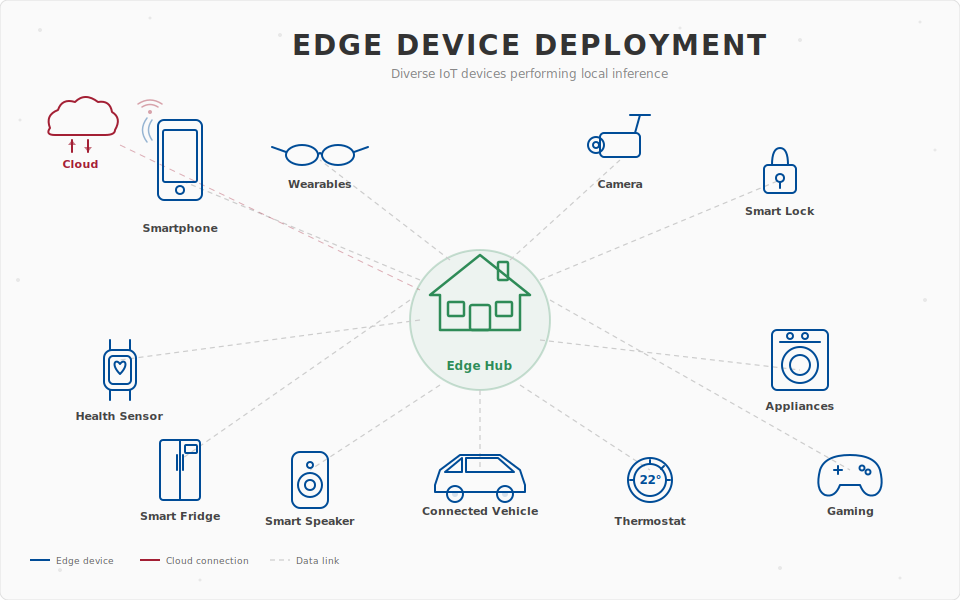
\includegraphics[keepaspectratio]{contents/vol1/ml_systems/images/jpg/edge_ml_iot.jpg}}

}

\caption{\label{fig-edgeml-example}\textbf{Edge Device Deployment}:
Diverse IoT devices, from wearables to home appliances, enable
decentralized machine learning by performing inference locally, reducing
reliance on cloud connectivity and improving response times. Source:
Edge Impulse.}

\end{figure}%

To make these trade-offs concrete, the following worked example applies
\emph{edge inference sizing} to a realistic retail deployment scenario.

\phantomsection\label{callout-notebookux2a-1.16}
\begin{fbx}{callout-notebook}{AI Engineer’s Notebook:}{Edge Inference Sizing}
\phantomsection\label{callout-notebook*-1.16}
\textbf{Scenario}: A smart retail chain deploying person detection
across 500 stores, each with 20 cameras at 15 FPS.

\textbf{Requirements Analysis}

\begin{longtable}[]{@{}
  >{\raggedright\arraybackslash}p{(\linewidth - 4\tabcolsep) * \real{0.2015}}
  >{\raggedright\arraybackslash}p{(\linewidth - 4\tabcolsep) * \real{0.4925}}
  >{\raggedright\arraybackslash}p{(\linewidth - 4\tabcolsep) * \real{0.2985}}@{}}
\toprule\noalign{}
\begin{minipage}[b]{\linewidth}\raggedright
\textbf{Metric}
\end{minipage} & \begin{minipage}[b]{\linewidth}\raggedright
\textbf{Calculation}
\end{minipage} & \begin{minipage}[b]{\linewidth}\raggedright
\textbf{Result}
\end{minipage} \\
\midrule\noalign{}
\endhead
\bottomrule\noalign{}
\endlastfoot
\textbf{Inferences per store} &
\multicolumn{2}{>{\raggedright\arraybackslash}p{(\linewidth - 4\tabcolsep) * \real{0.7910} + 2\tabcolsep}@{}}{%
20 cameras × 15 FPS \textbar{} 300 inferences/sec \textbar{}} \\
\textbf{Model compute} &
\multicolumn{2}{>{\raggedright\arraybackslash}p{(\linewidth - 4\tabcolsep) * \real{0.7910} + 2\tabcolsep}@{}}{%
YOLOv8-nano: 3.2 GFLOPs/inference \textbar{} 960 GFLOPs/sec
\textbar{}} \\
\textbf{Required throughput} &
\multicolumn{2}{>{\raggedright\arraybackslash}p{(\linewidth - 4\tabcolsep) * \real{0.7910} + 2\tabcolsep}@{}}{%
960 GFLOPs × 2 (headroom) \textbar{} \textasciitilde2 TFLOPS
\textbar{}} \\
\end{longtable}

\textbf{Hardware Selection}

\begin{longtable}[]{@{}
  >{\raggedright\arraybackslash}p{(\linewidth - 8\tabcolsep) * \real{0.2074}}
  >{\raggedleft\arraybackslash}p{(\linewidth - 8\tabcolsep) * \real{0.1185}}
  >{\raggedright\arraybackslash}p{(\linewidth - 8\tabcolsep) * \real{0.2148}}
  >{\raggedright\arraybackslash}p{(\linewidth - 8\tabcolsep) * \real{0.1926}}
  >{\raggedleft\arraybackslash}p{(\linewidth - 8\tabcolsep) * \real{0.2444}}@{}}
\toprule\noalign{}
\begin{minipage}[b]{\linewidth}\raggedright
\textbf{Edge Device}
\end{minipage} & \begin{minipage}[b]{\linewidth}\raggedleft
\textbf{INT8 TOPS}
\end{minipage} & \begin{minipage}[b]{\linewidth}\raggedright
\textbf{Power}
\end{minipage} & \begin{minipage}[b]{\linewidth}\raggedright
\textbf{Unit Cost}
\end{minipage} & \begin{minipage}[b]{\linewidth}\raggedleft
\textbf{Fleet Cost}
\end{minipage} \\
\midrule\noalign{}
\endhead
\bottomrule\noalign{}
\endlastfoot
\textbf{NVIDIA Jetson Orin NX} & 100 TOPS & 10-40 W &
\multicolumn{2}{>{\raggedright\arraybackslash}p{(\linewidth - 8\tabcolsep) * \real{0.4370} + 2\tabcolsep}@{}}{%
\$600 \textbar{} \$300,000 \textbar{}} \\
\textbf{Intel NUC + Movidius} & 4 TOPS & 15 W & \$400 & \$200,000 \\
\textbf{Google Coral Dev} & 4 TOPS &
\multicolumn{3}{>{\raggedright\arraybackslash}p{(\linewidth - 8\tabcolsep) * \real{0.6519} + 4\tabcolsep}@{}}{%
2 W \textbar{} \$150 \textbar{} \$75,000 \textbar{}} \\
\end{longtable}

\textbf{Decision}: At 2 TFLOPS required and INT8 quantization providing
\textasciitilde4× effective throughput, the Coral Dev Board (4 TOPS)
meets requirements at 1/4 the cost of Jetson, with 12× lower power
consumption.

\textbf{TCO over 3 years} (Coral): Hardware \$75K + Power
(\$2×500×8760h×3yr×\$0.12/kWh) = \$75K + \$3K = \textbf{\$78,000 total}
vs.~cloud inference at \textasciitilde\$500K.

\end{fbx}

\subsection{Real-Time Industrial and IoT
Systems}\label{sec-ml-system-architecture-realtime-industrial-iot-systems-373a}

Industries deploy Edge ML widely where low latency, data privacy, and
operational resilience justify the additional complexity. Autonomous
vehicles represent the most demanding application, where safety-critical
decisions must occur within milliseconds based on sensor data that
cannot be transmitted to remote servers. Systems like Tesla's Full
Self-Driving process inputs from multiple cameras at high frame rates
through custom edge hardware, making driving decisions with end-to-end
latency on the order of milliseconds. This response time is infeasible
with cloud processing due to network delays.

Smart retail environments demonstrate edge ML's practical advantages for
privacy-sensitive, bandwidth-intensive applications. Amazon
Go\sidenote{\textbf{Amazon Go}: Launched in 2018, this checkout-free
retail concept demonstrates edge ML at scale. Each store deploys
hundreds of cameras and shelf sensors processed by local GPU clusters
running multi-object tracking, pose estimation, and activity
recognition. The system must process \textasciitilde1 TB/hour of video
data locally because cloud transmission would require impractical
bandwidth (100+ Mbps sustained) and add unacceptable latency for
real-time tracking. } stores process video from hundreds of cameras
through local edge servers, tracking customer movements and item
selections to enable checkout-free shopping. This edge-based approach
addresses both technical and privacy concerns. Transmitting
high-resolution video from hundreds of cameras would require substantial
sustained bandwidth, while local processing keeps raw video on premises,
reducing exposure and simplifying compliance.

The Industrial IoT\sidenote{\textbf{Industry 4.0}: Fourth industrial
revolution (term coined 2011 at Hannover Fair) integrating AI, IoT, and
cyber-physical systems into manufacturing. Digital twins simulate
production lines; ML optimizes scheduling and quality control. Industry
analyses project significant productivity gains and cost reductions
across global manufacturing through smart factory adoption
(\citeproc{ref-mckinsey2021iot}{Epstein 2017}). } leverages edge ML for
applications where millisecond-level responsiveness directly impacts
production efficiency and worker safety. Manufacturing facilities deploy
edge ML systems for real-time quality control. Vision systems inspect
welds at speeds exceeding 60 parts per minute. Predictive
maintenance\sidenote{\textbf{Predictive Maintenance}: ML-driven
maintenance scheduling analyzing vibration, temperature, and acoustic
signatures to predict equipment failures. Industry deployments report
significant reductions in unplanned downtime, maintenance costs, and
extended equipment life. Large-scale industrial IoT platforms monitor
millions of assets, demonstrating substantial savings through failure
avoidance (\citeproc{ref-mckinsey2021iot}{Epstein 2017}). } applications
monitor over 10,000 industrial assets per facility. This approach has
demonstrated 25-35\% reductions in unplanned downtime across various
manufacturing sectors.

Smart buildings utilize edge ML to optimize energy consumption while
maintaining operational continuity during network outages. Commercial
buildings equipped with edge-based building management systems process
data from thousands of sensors monitoring temperature, occupancy, air
quality, and energy usage. This reduces cloud transmission requirements
by an order of magnitude or more while enabling sub-second response
times. Healthcare applications similarly leverage edge ML for patient
monitoring and surgical assistance, maintaining HIPAA compliance through
local processing while supporting low-latency workflows for real-time
guidance.

\section{Mobile ML: Personal and Offline
Intelligence}\label{sec-ml-system-architecture-mobile-ml-personal-offline-intelligence-0983}

Edge ML solves the distance problem that limits cloud deployments,
achieving sub-100 ms latency through local processing. However, edge
devices remain tethered to stationary infrastructure---gateways, factory
servers, retail edge systems---limiting where intelligence can be
deployed. To bring ML capabilities to users in motion, we must solve a
different constraint: the \textbf{Battery}. Unlike plugged-in edge
servers that can consume hundreds of watts continuously, mobile devices
must operate for hours or days on fixed energy budgets.

Mobile ML addresses this challenge by integrating machine learning
directly into portable devices like smartphones and tablets, providing
users with real-time, personalized capabilities. This paradigm excels
when user privacy, offline operation, and immediate responsiveness
matter more than computational sophistication, supporting applications
such as voice recognition\sidenote{\textbf{Voice Recognition Evolution}:
Apple Siri (2011) required cloud processing with 200-500ms latency and
privacy concerns. By 2017, on-device models reduced latency to
\textless50ms while keeping audio local. Modern NPUs process 16kHz audio
in 20-30ms using transformer-based models; Google's on-device
transcription achieves 95\%+ accuracy entirely locally. }, computational
photography\sidenote{\textbf{Computational Photography}: Combines
multiple exposures and ML algorithms to enhance image quality. Google's
Night Sight captures 15 frames in 6 seconds, using ML to align and merge
them. Portrait mode uses depth estimation ML models to create
professional-looking bokeh effects in real-time. }, and health
monitoring while maintaining data privacy through on-device computation.
These battery-powered devices must balance performance with power
efficiency and thermal management, making them suited to frequent,
short-duration AI tasks.

The mobile environment introduces a critical constraint absent from
stationary deployments: \emph{energy per inference} becomes a
first-order design parameter. A \textbf{Compute Beast} workload like
image classification must be transformed through architectural
efficiency (e.g., depthwise separable
convolutions\sidenote{\textbf{Depthwise Separable Convolutions}:
Architectural innovation introduced by MobileNet (2017) that factorizes
standard convolutions into depthwise and pointwise operations. For a
\(D_K \times D_K\) kernel on \(M\) input channels producing \(N\)
outputs, standard convolution costs \(D_K^2 \times M \times N\)
multiplications, while depthwise separable costs
\(D_K^2 \times M + M \times N\), yielding 8-9x reduction for typical
parameters. This efficiency enables running vision models within mobile
power budgets. } in MobileNet) to reduce FLOPs by 8-9× while preserving
accuracy. This is not merely optimization; it represents a fundamental
shift in the arithmetic intensity trade-off, accepting lower peak
throughput in exchange for sustainable operation within a 3-5 W thermal
envelope.

We define this paradigm formally as \emph{Mobile ML}.

\phantomsection\label{callout-definitionux2a-1.17}
\begin{fbx}{callout-definition}{Definition:}{Mobile ML}
\phantomsection\label{callout-definition*-1.17}
\textbf{\emph{Mobile Machine Learning}} is the deployment paradigm
bounded by \textbf{Thermal Design Power (TDP)}. Unlike cloud systems
constrained by cost, Mobile ML is limited by the \textbf{Heat
Dissipation} capacity of passive cooling (typically 3--5W) and total
battery energy, requiring architectures that trade peak throughput for
\textbf{Sustained Energy Efficiency}.

\end{fbx}

Figure~\ref{fig-mobile-ml} contrasts the unique characteristics of
mobile deployment. The \textbf{Characteristics} branch emphasizes sensor
integration (cameras, GPS), which enables the key \textbf{Benefit} of
context awareness. However, the \textbf{Challenges} branch reveals the
``Thermal Wall'' and battery limits that force engineers to optimize for
efficiency over raw performance.

\begin{figure}[t]

\centering{

\pandocbounded{\includegraphics[keepaspectratio]{index_files/mediabag/f467cf2b8ad822aa42a0d506596bbb1694207553.pdf}}

}

\caption{\label{fig-mobile-ml}\textbf{Mobile ML Decomposition.}
Characteristics, benefits, challenges, and representative applications
of mobile machine learning, where on-device processing and hardware
acceleration balance computational efficiency, battery life, and model
performance on smartphones and tablets.}

\end{figure}%

The battery life and resource constraints listed above translate
directly into engineering requirements. Consider the implications for
always-on ML features.

\phantomsection\label{callout-notebookux2a-1.18}
\begin{fbx}{callout-notebook}{AI Engineer’s Notebook:}{The Battery Tax}
\phantomsection\label{callout-notebook*-1.18}
\textbf{Problem}: You want to deploy a ``real-time'' background object
detector on a smartphone. The model consumes \textbf{2 Watts} of
continuous power when active. The phone has a standard \textbf{15
Watt-hour (Wh)} battery.

\textbf{The Physics}:

\begin{enumerate}
\def\labelenumi{\arabic{enumi}.}
\tightlist
\item
  \textbf{Ideal Runtime}:
  \(15 \text{ Wh} / 2 \text{ W} = \mathbf{7\.5 \text{ hours}}\).
\item
  \textbf{The Reality}: A user expects their phone to last 24 hours.
  Your single feature has just consumed \textbf{100\%} of the entire
  daily energy budget in a few hours.
\end{enumerate}

\textbf{The Engineering Conclusion}: You cannot simply ``deploy'' the
model. You must use the techniques in \textbf{?@sec-model-compression}
(quantization, duty-cycling) to reduce the power to \textbf{\textless100
mW} if you want it to stay on all day.

\end{fbx}

The battery constraint limits total energy consumption over time.
However, even if we could ignore battery life---perhaps for a plugged-in
tablet or a short demo---a second physical law intervenes:
thermodynamics. Every watt of computation becomes a watt of heat that
must be dissipated. In a data center, massive cooling systems remove
this heat. In a thin, sealed mobile device with no fan, the only heat
path is through the glass and metal casing to the surrounding air. This
thermal reality creates a hard ceiling on sustained power consumption
that exists independently of battery capacity.

\phantomsection\label{callout-notebookux2a-1.19}
\begin{fbx}{callout-notebook}{AI Engineer’s Notebook:}{The Thermal Wall}
\phantomsection\label{callout-notebook*-1.19}
\textbf{Problem}: Your unoptimized LLM requires \textbf{10 W} peak
compute. Can you deploy it on a mobile device?

\textbf{The Physics}:

\begin{enumerate}
\def\labelenumi{\arabic{enumi}.}
\tightlist
\item
  \textbf{Thermal Design Power (TDP)}: A mobile SoC allows
  \(\approx \mathbf{3 \text{ W}}\) for passive cooling.
\item
  \textbf{Temperature Rise}: At 10 W, the device temperature rises at
  \(\approx 1^\circ\text{C}\) per second.
\item
  \textbf{Thermal Trip}: Within 60 seconds, the hardware reaches the
  \textbf{Thermal Trip Point} (\(80^\circ\text{C}\)), triggering OS
  throttling.
\item
  \textbf{The Result}: Your 100 FPS model suddenly drops to \textbf{30
  FPS} to avoid melting the hardware.
\end{enumerate}

\textbf{The Engineering Conclusion}: Quantization from FP32 to INT8
reduces power by approximately 4×, but if the baseline power is 12W, you
are still at 3W---the absolute limit of the hardware. Physics sets a
hard ceiling that no optimization can exceed.

\end{fbx}

\phantomsection\label{sec-ml-system-architecture-battery-thermal-constraints-ab51}{}

\subsection{Mobile ML Benefits and Resource
Constraints}\label{sec-ml-system-architecture-mobile-ml-benefits-resource-constraints-c568}

\textbf{Battery and Thermal Constraints.} Mobile devices exemplify
intermediate constraints: 8-24GB RAM (varying from mid-range to
flagship), 128GB-1TB storage, 1-10 TOPS AI compute through Neural
Processing Units\sidenote{\textbf{Neural Processing Unit (NPU)}:
Specialized processors optimized for efficient neural network inference
on mobile devices. NPUs achieve high inference performance within tight
power budgets, enabling on-device AI. We examine NPU architectures and
their performance characteristics in \textbf{?@sec-ai-acceleration}. }
consuming 3-5W power. System-on-Chip
architectures\sidenote{\textbf{Mobile System-on-Chip (SoC)}:
Heterogeneous processors integrating CPU, GPU, NPU, ISP, and memory
controller on a single die. Apple's A17 Pro (3nm, 19B transistors)
delivers 35 TOPS via its 16-core Neural Engine; Qualcomm's Snapdragon 8
Gen 3 delivers approximately 34 TOPS through its Hexagon NPU. SoC
integration reduces data movement energy 10-100× compared to discrete
components. } integrate computation and memory to minimize energy costs.
Memory bandwidth of 25-50 GB/s limits models to 10-100MB parameters,
requiring the aggressive optimization techniques that
\textbf{?@sec-model-compression} details. Battery constraints (18-22Wh
capacity) make energy optimization critical: 1W continuous ML processing
reduces device lifetime from 24 to 18 hours. Specialized frameworks
(TensorFlow Lite\sidenote{\textbf{TensorFlow Lite}: Google's
mobile/embedded ML framework (2017) optimizing models through
quantization, pruning, and operator fusion. Supports Android, iOS,
Linux, and microcontrollers. Deploys on 4B+ devices running applications
from Google Translate (35MB multilingual model) to on-device speech
recognition with \textless100ms latency. }, Core
ML\sidenote{\textbf{Core ML}: Apple's on-device ML framework (iOS 11,
2017) with automatic optimization for Apple Silicon. Seamlessly
schedules across CPU, GPU, and Neural Engine based on model
characteristics. Supports vision, NLP, and audio models from 1 KB--1 GB
with compiler optimizations achieving 2--10\(\times\) speedups over
naive deployment. }) provide hardware-optimized inference enabling
\textless50ms UI response times.

Mobile ML excels at delivering responsive, privacy-preserving user
experiences. Real-time processing can reach sub-10 ms latency for some
tasks, enabling imperceptible response in interactive applications.
Stronger privacy properties emerge when sensitive inputs are processed
locally, reducing data transmission and central storage, though privacy
still depends on system design and threat model. On-device enclaves and
similar hardware isolation mechanisms can help protect sensitive
computations (for example, biometric processing)\sidenote{\textbf{Mobile
Face Detection}: Apple's Face ID projects 30,000 IR dots for 3D face
mapping, processed entirely in the Secure Enclave (isolated
cryptographic coprocessor). Biometric templates never leave the device;
even Apple cannot access them. Achieves 1:1,000,000 false acceptance
rate vs.~Touch ID's 1:50,000, demonstrating privacy-preserving edge AI.
}. Offline functionality reduces network dependency: navigation,
translation\sidenote{\textbf{Real-Time Translation}: On-device neural
machine translation processing 40+ language pairs without internet
connectivity. Google Translate's offline models (35-45MB per language)
achieve 90\% of cloud quality (2GB+ models) through knowledge
distillation and quantization. Enables privacy-preserving translation
with \textless500ms latency on mid-range smartphones. }, and media
processing can run locally within mobile resource budgets.
Personalization improves because models can leverage on-device signals
and user context while keeping raw data local.

These benefits require accepting significant resource constraints.
Compared to cloud deployments, mobile applications often operate under
much tighter memory, storage, and latency budgets, which constrains
model size and batch behavior. Battery life\sidenote{\textbf{Mobile
Device Constraints}: Flagship phones (12-24GB RAM, 15-25W peak power)
operate with 10-100× less resources than cloud servers (256-2048GB RAM,
200-400W). Thermal throttling limits sustained performance; battery life
requires \textless500mW average inference power. These constraints drove
innovations in efficient architectures (MobileNet, EfficientNet) and
on-device optimization. } presents visible user impact, and thermal
throttling can materially limit sustained performance: peak NPU
throughput is often substantially higher than what is sustainable under
prolonged workloads. Development complexity multiplies across platforms,
demanding separate implementations and careful performance tuning, while
device heterogeneity requires multiple model variants. Deployment
friction adds further challenges: app store review processes can take
days, which can slow iteration relative to many cloud deployment
workflows.

\subsection{Personal Assistant and Media
Processing}\label{sec-ml-system-architecture-personal-assistant-media-processing-98d7}

Mobile ML has achieved success across diverse applications for billions
of users worldwide. Computational photography transformed smartphone
cameras into sophisticated imaging systems. Modern flagships process
every photo through multiple ML pipelines operating in real-time:
portrait mode\sidenote{\textbf{Portrait Mode Photography}: Computational
photography using ML segmentation to separate subjects from backgrounds,
applying synthetic depth-of-field effects mimicking DSLR bokeh. Dual
cameras or LiDAR provide depth estimation; neural networks refine edges
around hair and translucent objects. Processing occurs in real-time
(\textless100ms) on NPUs, enabling live preview before capture. } uses
depth estimation and segmentation networks to achieve DSLR-quality bokeh
effects, night mode captures and aligns 9-15 frames with ML-based
denoising that reduces noise by 10-20dB, and systems like Google Pixel
process 10-15 distinct ML models per photo for HDR merging,
super-resolution, and scene optimization.

Voice-driven interactions demonstrate mobile ML's transformation of
human-device communication. These systems combine ultra-low-power
wake-word detection consuming less than 1mW with on-device speech
recognition achieving under 10ms latency for simple commands. Keyboard
prediction has evolved to context-aware neural models achieving 60-70\%
phrase prediction accuracy, reducing typing effort by 30-40\%. Real-time
camera translation processes over 100 languages at 15-30fps entirely
on-device, enabling instant visual translation without internet
connectivity.

Health monitoring through wearables like Apple Watch extracts
sophisticated insights from sensor data while maintaining complete
privacy. These systems achieve over 95\% accuracy in activity detection
and include FDA-cleared atrial fibrillation detection with 98\%+
sensitivity, processing extraordinarily sensitive health data entirely
on-device to maintain HIPAA compliance. Accessibility features
demonstrate transformative social impact through continuous local
processing: Live Text detects and recognizes text from camera feeds,
Sound Recognition alerts deaf users to environmental cues through haptic
feedback, and VoiceOver generates natural language descriptions of
visual content.

Augmented reality frameworks leverage mobile ML for real-time
environment understanding at 60fps. ARCore and ARKit track device
position with centimeter-level accuracy while simultaneously mapping 3D
surroundings, enabling hand tracking that extracts 21-joint 3D poses and
face analysis of 50+ landmark meshes for real-time effects. These
applications demand consistent sub-16ms frame times, making only
on-device processing viable for delivering the seamless experiences
users expect.

Despite mobile ML's demonstrated capabilities, a common pitfall involves
attempting to deploy desktop-trained models directly to mobile or edge
devices without architecture modifications. Models developed on powerful
workstations often fail when deployed to resource-constrained devices. A
ResNet-50 model requiring 4 GB memory for inference (including
activations and batch processing) and 4 billion FLOPs per inference
cannot run on a device with 512 MB of RAM and a 1 GFLOP/s processor.
Beyond simple resource violations, desktop-optimized models may use
operations unsupported by mobile hardware (specialized mathematical
operations), assume floating-point precision unavailable on embedded
systems, or require batch processing incompatible with single-sample
inference. Successful deployment demands architecture-aware design from
the beginning, including specialized architectural techniques for mobile
devices (\citeproc{ref-howard2017mobilenets}{Howard et al. 2017}),
integer-only operations for microcontrollers, and optimization
strategies that maintain accuracy while reducing computation.

\section{TinyML: Ubiquitous Sensing at
Scale}\label{sec-ml-system-architecture-tinyml-ubiquitous-sensing-scale-a67b}

Mobile ML brings intelligence to users on the move, but smartphones cost
hundreds to thousands of dollars and are far too large to embed in
everyday objects. To put ``eyes and ears'' on every physical
object---from individual boxes in a warehouse to every leaf in a
field---we must push beyond mobile constraints entirely, solving for
both \textbf{cost} (dollars, not hundreds of dollars) and \textbf{size}
(millimeters, not centimeters).

TinyML (\citeproc{ref-reddi2022widening}{Janapa Reddi et al. 2022})
completes the deployment spectrum by pushing intelligence to its
physical limits. Devices costing less than \$10 and consuming less than
1 milliwatt of power make ubiquitous\sidenote{\textbf{Ubiquitous}: From
Latin \emph{ubique} (everywhere), combining \emph{ubi} (where) and the
generalizing suffix \emph{-que}. Mark Weiser at Xerox PARC coined
``ubiquitous computing'' in 1988 to describe technology so embedded in
the environment that it becomes invisible. TinyML realizes this vision:
when sensors cost dollars and run for years on a battery, intelligence
can literally be \emph{everywhere}, disappearing into the physical
world. } sensing economically practical at massive scale. This is the
exclusive domain of the \textbf{Tiny Constraint} Archetype, where the
optimization objective shifts from maximizing throughput to minimizing
energy per inference. A keyword spotting model consuming 10 µJ per
inference can operate for years on a coin-cell battery, achieving
million-fold improvements in energy efficiency by trading model capacity
for operational longevity.

Where mobile ML requires sophisticated hardware with gigabytes of memory
and multi-core processors, Tiny Machine Learning operates on
microcontrollers with kilobytes of RAM and single-digit dollar price
points. This radical constraint forces a shift in machine learning
deployment, prioritizing ultra-low power consumption and minimal cost
over computational sophistication.

TinyML brings intelligence to the smallest devices, from
microcontrollers\sidenote{\textbf{Microcontrollers}: Single-chip
computers with integrated CPU, memory, and peripherals, typically
operating at 1-100MHz with 32KiB-2MiB RAM. Arduino Uno uses an
ATmega328P with 32KiB flash and 2KiB RAM, while ESP32 provides WiFi
capability with 520KiB RAM, still thousands of times less than a
smartphone. } to embedded sensors, enabling real-time computation in
severely resource-constrained environments
(\citeproc{ref-banbury2021mlperftiny}{Banbury et al. 2021};
\citeproc{ref-lin2020mcunet}{Lin et al. 2020}). This paradigm excels in
applications requiring ubiquitous sensing, autonomous operation, and
maximal energy efficiency. TinyML systems power applications such as
predictive maintenance, environmental monitoring, and simple gesture
recognition while optimized for energy
efficiency\sidenote{\textbf{Energy Efficiency in TinyML}: Ultra-low
power enables decade-long deployment in remote locations. ARM Cortex-M0+
consumes \textless1µW in sleep, 100-300µW/MHz active. Specialized
accelerators (Syntiant NDP, MAX78000) achieve \textless1µJ per
inference. This 1,000,000\(\times\) gap between TinyML and cloud
inference energy drives entirely different system architectures and
deployment models. }, often running for months or years on limited power
sources such as coin-cell batteries\sidenote{\textbf{Coin-Cell
Batteries}: Compact power sources (CR2032: 225mAh at 3V) enabling
``deploy-and-forget'' IoT devices. TinyML models consuming 10-50µW
average power can operate 1-10 years on a single cell. Constrains models
to \textless100KB (fitting in on-chip SRAM), driving innovation in
efficient neural network architectures and intermittent computing
paradigms. }, as exemplified by the device kits in
Figure~\ref{fig-TinyML-example}. These systems deliver actionable
insights in remote or disconnected environments where power,
connectivity, and maintenance access are impractical.

\begin{figure}

\centering{

\pandocbounded{\includegraphics[keepaspectratio]{contents/vol1/ml_systems/images/png/tiny_ml.png}}

}

\caption{\label{fig-TinyML-example}\textbf{TinyML System Scale}: Small
development boards, including Arduino Nano BLE Sense and similar
microcontroller kits approximately 2 to 5 cm in length, with visible
processor chips and pin connectors that enable sensor integration for
always-on ML inference at milliwatt power budgets. Source:
(\citeproc{ref-warden2018speech}{Warden 2018})}

\end{figure}%

We define this paradigm formally as \emph{TinyML}.

\phantomsection\label{callout-definitionux2a-1.20}
\begin{fbx}{callout-definition}{Definition:}{TinyML}
\phantomsection\label{callout-definition*-1.20}
\textbf{\emph{TinyML}} is the domain of \textbf{Always-On Sensing}
constrained by \textbf{Kilobyte-Scale Memory} and
\textbf{Milliwatt-Scale Power}. It necessitates models small enough to
reside entirely in on-chip SRAM (avoiding the energy cost of DRAM
access) to enable continuous inference on energy-harvested or coin-cell
power sources.

\end{fbx}

TinyML's milliwatt-scale power consumption represents a
six-order-of-magnitude reduction from cloud inference, a gap with
profound implications for system design.

\phantomsection\label{callout-notebookux2a-1.21}
\begin{fbx}{callout-notebook}{AI Engineer’s Notebook:}{Energy Per Inference}
\phantomsection\label{callout-notebook*-1.21}
Energy consumption spans eight orders of magnitude across deployment
paradigms:

\begin{longtable}[]{@{}
  >{\raggedright\arraybackslash}p{(\linewidth - 6\tabcolsep) * \real{0.1531}}
  >{\raggedright\arraybackslash}p{(\linewidth - 6\tabcolsep) * \real{0.2347}}
  >{\raggedleft\arraybackslash}p{(\linewidth - 6\tabcolsep) * \real{0.2347}}
  >{\raggedleft\arraybackslash}p{(\linewidth - 6\tabcolsep) * \real{0.3571}}@{}}
\toprule\noalign{}
\begin{minipage}[b]{\linewidth}\raggedright
\textbf{Paradigm}
\end{minipage} & \begin{minipage}[b]{\linewidth}\raggedright
\textbf{Example Workload}
\end{minipage} & \begin{minipage}[b]{\linewidth}\raggedleft
\textbf{Energy/Inference}
\end{minipage} & \begin{minipage}[b]{\linewidth}\raggedleft
\textbf{Battery Life (3.7V, 3000mAh)}
\end{minipage} \\
\midrule\noalign{}
\endhead
\bottomrule\noalign{}
\endlastfoot
\textbf{Cloud} & GPT-4 query & \textasciitilde1 kJ & 0.01 queries \\
\textbf{Cloud} & ResNet-50 (A100) & \textasciitilde10 J & 1 query \\
\textbf{Edge} & ResNet-50 (Jetson) & \textasciitilde500 mJ & 20
queries \\
\textbf{Mobile} & MobileNet (NPU) & \textasciitilde50 mJ & 200
queries \\
\textbf{TinyML} & Keyword spotting & \textasciitilde10 µJ & 1 billion
inferences \\
\end{longtable}

\textbf{Key insight}: A TinyML wake-word detector at 10 µJ/inference is
\textbf{100,000,000×} more energy-efficient than a cloud LLM query. This
gap explains why always-on sensing is only practical at the TinyML
tier---a smartphone running continuous cloud queries would drain in
minutes.

\end{fbx}

Figure~\ref{fig-tiny-ml} maps TinyML's unique position. The
\textbf{Characteristics} branch reveals the extreme constraints:
milliwatt power and kilobyte memory. These limits enable the
\textbf{Benefit} of ``always-on'' sensing that no other paradigm can
sustain, but force engineers to solve the \textbf{Challenge} of extreme
model compression.

\begin{figure}[t]

\centering{

\pandocbounded{\includegraphics[keepaspectratio]{index_files/mediabag/a2593b8008f591c2d000319ac7df5783ff23f128.pdf}}

}

\caption{\label{fig-tiny-ml}\textbf{TinyML Decomposition.}
Characteristics, benefits, challenges, and representative applications
of TinyML, where milliwatt power budgets and kilobyte memory limits
enable always-on sensing and localized intelligence in embedded
applications.}

\end{figure}%

\phantomsection\label{sec-ml-system-architecture-extreme-resource-constraints-2273}{}

\subsection{TinyML Advantages and Operational
Trade-offs}\label{sec-ml-system-architecture-tinyml-advantages-operational-tradeoffs-2d40}

\textbf{Extreme Resource Constraints.} TinyML operates at hardware
extremes. Compared to cloud systems, TinyML deployments often have on
the order of (10\^{}4) to (10\^{}5) times less memory and power budgets
in the milliwatt range. Such strict limitations enable months or years
of autonomous operation\sidenote{\textbf{On-Device Training
Constraints}: Microcontrollers (256KiB-2MiB RAM) cannot support full
backpropagation through large networks. Alternatives include on-device
fine-tuning of final layers, federated learning with local gradient
computation, and TinyTL (memory-efficient training using
\textless50KiB). Apple's on-device personalization adapts keyboard
predictions without uploading typing data. } but demand specialized
algorithms and careful systems co-design. Devices range from palm-sized
developer kits to millimeter-scale chips\sidenote{\textbf{TinyML Device
Scale}: ML-capable chips range from 5×5mm (Syntiant NDP: 140µW, 1MiB
SRAM) to full single-board computers (Coral Dev Board Mini: 40×48mm, 4
TOPS). This 100× size range reflects diverse deployment needs from
implantable medical devices to industrial edge gateways processing
multiple sensor streams simultaneously. }, enabling ubiquitous sensing
in contexts where networking, power, or maintenance are costly.
Representative developer kits include the Arduino Nano 33 BLE Sense
(256KiB RAM, 1MiB flash, 20-40mW) and ESP32-CAM (520KiB RAM, 4MiB flash,
50-250mW).

TinyML's extreme resource constraints enable unique advantages that are
difficult to achieve at other scales. Avoiding network transmission
reduces end-to-end latency and eliminates communication overhead,
enabling rapid local responses for sensing and control loops. The
economics can be compelling for massive-scale deployments because
per-node costs can be low enough to instrument large physical
environments. Energy efficiency enables multi-year operation on small
batteries, and energy harvesting can further extend lifetimes in some
settings. Privacy improves because raw data can remain local, reducing
transmission and central storage, though this does not automatically
provide formal privacy guarantees without additional privacy and
security mechanisms.

These capabilities require substantial trade-offs. Computational
constraints impose severe limits: microcontrollers commonly provide on
the order of (10\^{}5) to (10\^{}6) bytes of RAM, which can force models
and intermediate activations into the tens of kilobytes to low megabytes
range, depending on the workload. Development complexity requires
expertise spanning neural network optimization, hardware-level memory
management, embedded toolchains, and specialized debugging across
diverse microcontroller architectures. Model quality can suffer from
aggressive compression and reduced precision, limiting suitability for
applications requiring high accuracy or robustness. Deployment can also
be inflexible: devices may run a small set of fixed models, and updates
may require firmware workflows that are slower and riskier than cloud
rollouts. Ecosystem fragmentation\sidenote{\textbf{TinyML Model
Optimization}: Compression techniques enable running ML on
microcontrollers by dramatically reducing model size while preserving
accuracy. Quantization, pruning, knowledge distillation, and
architecture search work together to achieve these reductions. Detailed
compression methods are covered in \textbf{?@sec-model-compression}. }
across microcontroller vendors and ML frameworks creates additional
overhead and portability challenges.

\subsection{Environmental and Health
Monitoring}\label{sec-ml-system-architecture-environmental-health-monitoring-14ad}

TinyML succeeds across domains where its advantages of ultra-low power,
low per-node cost, and local processing enable applications impractical
with other paradigms.

Wake-word detection represents a visible consumer application of TinyML,
where always-listening capabilities can be implemented at sub-milliwatt
continuous power consumption. These systems typically process audio
streams locally and only activate higher-power components when a wake
phrase is detected, reducing average device power
draw\sidenote{\textbf{TinyML in Fitness Trackers}: Wearables run
continuous ML inference on accelerometer, gyroscope, and heart rate
data. Apple Watch's fall detection analyzes motion patterns at 50Hz,
distinguishing falls from sitting down with high accuracy. Operating at
\textless1mW enables week-long battery life while monitoring health
metrics 24/7, a defining example of always-on TinyML. }.

Precision agriculture leverages TinyML's economic advantages where
traditional solutions prove cost-prohibitive. Deployments can instrument
thousands of monitoring points with multi-year battery operation,
transmitting summaries instead of raw sensor streams to reduce
connectivity costs.

Wildlife conservation uses TinyML for remote environmental monitoring.
Researchers deploy solar-powered audio sensors consuming 100-500mW that
process continuous audio streams for species identification. By
performing local analysis, these systems reduce satellite transmission
requirements from 4.3GB per day to 400KB of detection summaries, a
10,000x reduction that makes large-scale deployments of 100-1,000
sensors economically feasible. Medical wearables achieve FDA-cleared
cardiac monitoring with 95-98\% sensitivity while processing 250-500 ECG
samples per second at under 5mW power consumption. This efficiency
enables week-long continuous monitoring versus hours for
smartphone-based alternatives, while reducing diagnostic costs from
\$2,000-5,000 for traditional in-lab studies to under \$100 for at-home
testing.

\section{Comparative Analysis and Paradigm
Selection}\label{sec-ml-system-architecture-comparative-analysis-paradigm-selection-bf66}

The preceding four sections examined each deployment paradigm through
the same lens: definition, characteristics, trade-offs, and
applications. This parallel treatment revealed that each paradigm
emerged as a response to specific physical constraints. Cloud ML accepts
latency for unlimited compute, Edge ML trades compute for latency,
Mobile ML trades compute for portability, and TinyML trades compute for
ubiquity.

Now we step back to see the full picture. How do these paradigms compare
quantitatively across all dimensions? And given a specific application,
how should an engineer select among them? This section synthesizes the
individual paradigm analyses into a unified comparison framework and a
structured decision process.

\subsection{Quantitative Trade-off
Analysis}\label{sec-ml-system-architecture-quantitative-tradeoff-analysis-56a8}

The relationship between computational resources and deployment location
forms one of the most consequential comparisons across ML systems.
Moving from cloud deployments to tiny devices reveals a dramatic
reduction in available computing power, storage, and energy consumption.
Cloud ML systems leverage virtually unlimited resources, processing
petabytes of data and training models with billions of parameters. Edge
ML systems, while more constrained, still offer significant
computational capability through specialized hardware such as edge GPUs
and neural processing units. Mobile ML balances computational power with
energy efficiency on smartphones and tablets. At the far end of the
spectrum, TinyML operates under severe resource constraints, often
limited to kilobytes of memory and milliwatts of power consumption.

Table~\ref{tbl-big_vs_tiny} provides a comprehensive comparison across
fourteen dimensions, from compute power and latency to cost and
deployment speed.

\begin{longtable}[]{@{}
  >{\raggedright\arraybackslash}p{(\linewidth - 10\tabcolsep) * \real{0.1245}}
  >{\raggedright\arraybackslash}p{(\linewidth - 10\tabcolsep) * \real{0.1845}}
  >{\raggedright\arraybackslash}p{(\linewidth - 10\tabcolsep) * \real{0.1760}}
  >{\raggedright\arraybackslash}p{(\linewidth - 10\tabcolsep) * \real{0.1373}}
  >{\raggedright\arraybackslash}p{(\linewidth - 10\tabcolsep) * \real{0.2403}}
  >{\raggedright\arraybackslash}p{(\linewidth - 10\tabcolsep) * \real{0.1202}}@{}}
\caption{\textbf{Deployment Locations}: Machine learning systems vary in
where computation occurs, from centralized cloud servers to local edge
devices and ultra-low-power TinyML chips, each impacting latency,
bandwidth, and energy consumption. Deployments are categorized by
processing location and associated characteristics, enabling informed
decisions about system architecture and resource
allocation.}\label{tbl-big_vs_tiny}\tabularnewline
\toprule\noalign{}
\endfirsthead
\endhead
\bottomrule\noalign{}
\endlastfoot
\multirow{2}{=}{\textbf{Aspect} :===========================
\textbf{Processing Location}} & \multirow{2}{=}{\textbf{Cloud ML}
:========================================= Centralized cloud servers
(Data Centers)} & \multirow{2}{=}{\textbf{Edge ML}
:======================================= Local edge devices (gateways,
servers)} & \multirow{2}{=}{\textbf{Mobile ML}
:============================== Smartphones and tablets} &
\multirow{2}{=}{\textbf{TinyML}
:====================================================== Ultra-low-power
microcontrollers and embedded systems} & \\
& & & & & \\
\textbf{Latency} &
\multicolumn{5}{>{\raggedright\arraybackslash}p{(\linewidth - 10\tabcolsep) * \real{0.8584} + 8\tabcolsep}@{}}{%
100 ms-1000 ms+ \textbar{} 10-100 ms \textbar{} 5-50 ms \textbar{} 1-10
ms \textbar{}} \\
\textbf{Compute Power} &
\multicolumn{5}{>{\raggedright\arraybackslash}p{(\linewidth - 10\tabcolsep) * \real{0.8584} + 8\tabcolsep}@{}}{%
Very High (Multiple GPUs/TPUs) \textbar{} High (Edge GPUs) \textbar{}
Moderate (Mobile NPUs/GPUs) \textbar{} Very Low (MCU/tiny
processors)} \\
\textbf{Storage Capacity} &
\multicolumn{5}{>{\raggedright\arraybackslash}p{(\linewidth - 10\tabcolsep) * \real{0.8584} + 8\tabcolsep}@{}}{%
Unlimited (petabytes+) \textbar{} Large (terabytes) \textbar{} Moderate
(gigabytes) \textbar{} Very Limited (kilobytes-megabytes) \textbar{}} \\
\textbf{Energy Consumption} &
\multicolumn{5}{>{\raggedright\arraybackslash}p{(\linewidth - 10\tabcolsep) * \real{0.8584} + 8\tabcolsep}@{}}{%
Very High (kW-MW range) \textbar{} High (100 s W) \textbar{} Moderate
(1-10 W) \textbar{} Very Low (mW range) \textbar{}} \\
\textbf{Scalability} & Excellent (virtually unlimited) & Good (limited
by edge hardware) & Moderate (per-device scaling) & Limited (fixed
hardware) & \\
\textbf{Data Privacy} & Basic-Moderate (Data leaves device) & High (Data
stays in local network) & High (Data stays on phone) & Very High (Raw
data can remain local) & \\
\textbf{Connectivity Required} & Constant high-bandwidth & Intermittent
& Optional & None & \\
\textbf{Offline Capability} & None & Good & Excellent & Complete & \\
\textbf{Real-time Processing} & Dependent on network & Good & Very Good
& Excellent & \\
\textbf{Cost} &
\multicolumn{3}{>{\raggedright\arraybackslash}p{(\linewidth - 10\tabcolsep) * \real{0.4979} + 4\tabcolsep}}{%
High (\$1000s+/month) \textbar{} Moderate (\$100s-1000s) \textbar{} Low
(\$0-10s)} &
\multicolumn{2}{>{\raggedright\arraybackslash}p{(\linewidth - 10\tabcolsep) * \real{0.3605} + 2\tabcolsep}@{}}{%
\begin{minipage}[t]{\linewidth}\raggedright
Moderate (\$100s-1000s) \textbar{} Low (\$0-10s) \textbar{} Very Low
(\$1-10s) \textbar{}
\end{minipage}} \\
\textbf{Hardware Requirements} & Cloud infrastructure & Edge
servers/gateways & Modern smartphones & MCUs/embedded systems & \\
\textbf{Development Complexity} & High (cloud expertise needed) &
Moderate-High (edge+networking) & Moderate (mobile SDKs) & High
(embedded expertise) & \\
\textbf{Deployment Speed} & Fast & Moderate & Fast & Slow & \\
\end{longtable}

Table~\ref{tbl-big_vs_tiny} reveals clear gradients in latency from
cloud (100-1000ms) to edge (10-100ms) to mobile (5-50ms) to tiny
(1-10ms), and privacy properties that are often strongest when TinyML
keeps raw data local. Before we visualize these trade-offs graphically,
let us understand how they connect to the Workload Archetypes introduced
earlier.

These quantitative trade-offs map directly to the Workload Archetypes
introduced earlier. \textbf{Compute Beasts} and \textbf{Sparse Scatter}
workloads naturally gravitate toward cloud deployment, where raw TFLOPS
and memory capacity are abundant. \textbf{Bandwidth Hogs} span cloud and
edge depending on latency requirements --- cloud for batch processing,
edge for interactive applications. \textbf{Tiny Constraint} workloads
are exclusively TinyML, where the joules-per-inference metric dominates
all other considerations. Mobile deployment occupies the middle ground,
hosting efficiency-optimized variants of Compute Beast workloads (e.g.,
MobileNet instead of ResNet) that trade peak performance for sustainable
power consumption.

Figure~\ref{fig-op_char} visualizes performance and operational
characteristics across paradigms through radar plots. Plot a) contrasts
compute power and scalability where Cloud ML excels against latency and
energy efficiency where TinyML dominates, with Edge and Mobile ML
occupying intermediate positions.

\begin{figure}[t]

\centering{

\pandocbounded{\includegraphics[keepaspectratio]{index_files/mediabag/115af2be894fa141ac565f830835c62468c7470c.pdf}}

}

\caption{\label{fig-op_char}\textbf{Paradigm Comparison Radar Plots.}
Two radar plots quantify performance and operational characteristics
across cloud, edge, mobile, and TinyML paradigms. The left plot
contrasts compute power, latency, scalability, and energy efficiency;
the right plot contrasts connectivity, privacy, real-time capability,
and offline operation.}

\end{figure}%

Plot b) emphasizes operational dimensions where TinyML excels (privacy,
connectivity independence, offline capability) versus Cloud ML's
dependency on centralized infrastructure and constant connectivity.

Development complexity varies inversely with hardware capability: Cloud
and TinyML require deep expertise (cloud infrastructure and embedded
systems respectively), while Mobile and Edge leverage more accessible
SDKs and tooling. Cost structures show similar inversion: Cloud incurs
ongoing operational expenses (\$1000s+/month), Edge requires moderate
upfront investment (\$100s-1000s), Mobile leverages existing devices
(\$0-10s), and TinyML minimizes hardware costs (\$1-10s) while demanding
higher development investment.

A critical pitfall in deployment selection involves choosing paradigms
based solely on model accuracy metrics without considering system-level
constraints. Teams often select deployment strategies by comparing model
accuracy in isolation, overlooking critical system requirements that
determine real-world viability. A cloud-deployed model achieving 99\%
accuracy becomes useless for autonomous emergency braking if network
latency exceeds reaction time requirements. Similarly, a sophisticated
edge model that drains a mobile device's battery in minutes fails
despite superior accuracy. Successful deployment requires evaluating
multiple dimensions simultaneously: latency requirements, power budgets,
network reliability, data privacy regulations, and total cost of
ownership. Establish these constraints before model development to avoid
expensive architectural pivots late in the project.

\subsection{Decision
Framework}\label{sec-ml-system-architecture-decision-framework-241f}

Selecting the appropriate deployment paradigm requires systematic
evaluation of application constraints rather than organizational biases
or technology trends. Figure~\ref{fig-mlsys-playbook-flowchart} provides
a hierarchical decision framework that filters options through critical
requirements: privacy, latency, computational demands, and cost
constraints.

\begin{figure}[t]

\centering{

\pandocbounded{\includegraphics[keepaspectratio]{index_files/mediabag/def1458f3d1cee8f92270c7c30a2552b51236a0e.pdf}}

}

\caption{\label{fig-mlsys-playbook-flowchart}\textbf{Deployment Decision
Logic}: This flowchart guides selection of an appropriate machine
learning deployment paradigm by systematically evaluating privacy
requirements and processing constraints, ultimately balancing
performance, cost, and data security. Navigating the decision tree helps
practitioners determine whether cloud, edge, mobile, or tiny machine
learning best suits a given application.}

\end{figure}%

The framework evaluates four critical decision layers sequentially.
Privacy constraints form the first filter, determining whether data can
be transmitted externally. Applications handling sensitive data under
GDPR, HIPAA, or proprietary restrictions mandate local processing,
immediately eliminating cloud-only deployments. Latency requirements
establish the second constraint through response time budgets:
applications requiring sub-10 ms response times cannot use cloud
processing, as physics-imposed network delays alone exceed this
threshold. Computational demands form the third evaluation layer,
assessing whether applications require high-performance infrastructure
that only cloud or edge systems provide, or whether they can operate
within the resource constraints of mobile or tiny devices. Cost
considerations complete the framework by balancing capital expenditure,
operational expenses, and energy efficiency across expected deployment
lifetimes.

The following worked example applies this framework step by step to a
safety-critical application: \emph{autonomous vehicle emergency
braking}.

\phantomsection\label{callout-notebookux2a-1.22}
\begin{fbx}{callout-notebook}{AI Engineer’s Notebook:}{Autonomous Vehicle Emergency Braking}
\phantomsection\label{callout-notebook*-1.22}
\textbf{Application}: Vision-based pedestrian detection for emergency
braking.

\textbf{Walking through the decision framework}:

\begin{enumerate}
\def\labelenumi{\arabic{enumi}.}
\tightlist
\item
  \textbf{Privacy}: Vehicle camera data is not transmitted to third
  parties → No strong privacy constraint. \emph{Could use cloud.}
\item
  \textbf{Latency}: Emergency braking requires \textless100 ms total
  response. At 60 mph, a car travels 2.7 meters in 100 ms.

  \begin{itemize}
  \tightlist
  \item
    Network latency to cloud: 50-150 ms (variable) → \textbf{Fails
    requirement}
  \item
    Edge processing: 10-30 ms → \textbf{Passes}
  \item
    \emph{Decision: Cloud eliminated by physics.}
  \end{itemize}
\item
  \textbf{Compute}: Pedestrian detection requires \textasciitilde10
  GFLOPs at 30 FPS = 300 GFLOPs/s sustained.

  \begin{itemize}
  \tightlist
  \item
    TinyML (\textless1 GFLOP/s): \textbf{Fails}
  \item
    Mobile NPU (\textasciitilde35 TOPS): Possible but thermal
    constraints limit sustained operation
  \item
    Edge GPU (\textasciitilde10+ TFLOPS): \textbf{Passes with margin}
  \item
    \emph{Decision: Edge or high-end Mobile.}
  \end{itemize}
\item
  \textbf{Cost}: Safety-critical, high-volume production (millions of
  vehicles).

  \begin{itemize}
  \tightlist
  \item
    Edge GPU: \$500-1000 per vehicle, amortized over 10+ year vehicle
    life = \$50-100/year
  \item
    \emph{Decision: Edge GPU justified for safety-critical application.}
  \end{itemize}
\end{enumerate}

\textbf{Result}: Edge ML with local GPU (NVIDIA Drive Orin class). Cloud
used only for training, model updates, and fleet-wide analytics---not
real-time inference.

\textbf{Key insight}: Latency constraints eliminated 75\% of options
before we considered compute or cost.

\end{fbx}

The decision framework above identifies technically feasible options,
but feasibility does not guarantee success. Production deployment also
depends on organizational capabilities that determine whether a
technically sound choice can be implemented and maintained effectively.

Successful deployment requires considering factors beyond pure
engineering constraints. Organizational factors shape success by
determining whether teams possess the capabilities to implement and
maintain chosen paradigms. Team expertise must align with paradigm
requirements: Cloud ML demands distributed systems knowledge, Edge ML
requires device management capabilities, Mobile ML needs
platform-specific optimization skills, and TinyML requires embedded
systems expertise. Organizations lacking appropriate skills face
extended development timelines and ongoing maintenance challenges that
undermine technical advantages. Monitoring and maintenance capabilities
similarly determine viability at scale: edge deployments require
distributed device orchestration, while TinyML demands specialized
firmware management that many organizations lack. Cost structures
further complicate decisions through their temporal patterns: Cloud
incurs recurring operational expenses favorable for unpredictable
workloads, Edge requires substantial upfront investment offset by lower
ongoing costs, Mobile leverages user-provided devices to minimize
infrastructure expenses, and TinyML minimizes hardware and connectivity
costs while demanding significant development investment.

These organizational realities raise a broader question: given the
infrastructure, expertise, and maintenance burden that ML systems
require, is a machine learning approach always the right choice? Every
ML deployment carries a \emph{complexity tax} that must be weighed
against simpler alternatives.

\phantomsection\label{callout-perspectiveux2a-1.23}
\begin{fbx}{callout-perspective}{Systems Perspective:}{The Complexity Tax}
\phantomsection\label{callout-perspective*-1.23}
Before committing to any ML deployment, weigh the \textbf{Complexity
Tax} against simpler alternatives.

Consider a classification problem solvable by either a
\textbf{Heuristic} (if-then rules) or a \textbf{Deep Learning Pipeline}:

\begin{enumerate}
\def\labelenumi{\arabic{enumi}.}
\tightlist
\item
  \textbf{The Heuristic}: 50 lines of code. Near-zero compute cost.
  Maintenance: \textasciitilde1 hour/month to update rules. No drift.
\item
  \textbf{The ML System}: 50 lines of model code + 2,000 lines of
  infrastructure (data pipelines, monitoring, GPU drivers). Maintenance:
  \textasciitilde40 hours/month debugging drift and managing
  infrastructure.
\end{enumerate}

If the ML system provides 95\% accuracy and the heuristic provides 90\%,
is that 5\% gain worth a \textbf{40× increase} in complexity? ML systems
engineering is the art of minimizing this tax through robust
architecture. If you cannot afford the operational cost to maintain
model quality over time, the simpler heuristic may be the superior
systems choice.

\end{fbx}

This complexity tax applies to every deployment decision. Before
proceeding to hybrid architectures, reflect on how you would make this
trade-off in your own systems.

\phantomsection\label{callout-checkpointux2a-1.24}
\begin{fbx}{callout-checkpoint}{Checkpoint:}{System Design}
\phantomsection\label{callout-checkpoint*-1.24}

The central trade-off is often \textbf{Accuracy vs.~Complexity}.

\textbf{Decision Gates}

\begin{itemize}
\tightlist
\item[$\square$]
  \textbf{The Baseline}: Have you measured the accuracy of a simple
  heuristic (regex, logistic regression) before training a Deep Network?
\item[$\square$]
  \textbf{The Infrastructure Cost}: Is the 2\% accuracy gain from a
  Transformer worth the 10x inference cost and maintenance burden
  compared to a smaller model?
\end{itemize}

\end{fbx}

Successful deployment emerges from balancing technical optimization
against organizational capability. Paradigm selection represents systems
engineering challenges that extend well beyond pure technical
requirements, encompassing team skills, operational capacity, and
economic constraints. These decisions remain constrained by fundamental
scaling laws, with operational aspects detailed in
\textbf{?@sec-machine-learning-operations-mlops} and benchmarking
approaches covered in \textbf{?@sec-benchmarking-ai}.

\section{Hybrid Architectures: Combining
Paradigms}\label{sec-ml-system-architecture-hybrid-architectures-combining-paradigms-7cdd}

The decision framework (Figure~\ref{fig-mlsys-playbook-flowchart}) helps
select the best single paradigm for a given application. In practice,
however, production systems rarely use just one paradigm. Voice
assistants combine TinyML wake-word detection with mobile speech
recognition and cloud natural language understanding. Autonomous
vehicles pair edge inference for real-time perception with cloud
training for model updates. These hybrid architectures leverage the
strengths of multiple paradigms while mitigating their individual
weaknesses. This section formalizes the integration strategies that make
such combinations effective.

\phantomsection\label{callout-definitionux2a-1.25}
\begin{fbx}{callout-definition}{Definition:}{Hybrid ML}
\phantomsection\label{callout-definition*-1.25}
\textbf{\emph{Hybrid Machine Learning}} is the architectural strategy of
\textbf{Hierarchical Distribution}. It partitions the ML workload across
the \textbf{Latency-Compute Pareto Frontier}, placing latency-critical
tasks on Edge/Tiny devices and throughput-intensive tasks in the Cloud,
linked by a unified data fabric.

\end{fbx}

\subsection{Integration
Patterns}\label{sec-ml-system-architecture-integration-patterns-5935}

Three essential patterns address common integration challenges:

\textbf{Train-Serve Split}: Training occurs in the cloud while inference
happens on edge, mobile, or tiny devices. This pattern leverages cloud
scale for training while benefiting from local inference latency and
privacy. Training costs may reach millions of dollars for large models,
while inference costs mere cents per query when deployed
efficiently.\sidenote{\textbf{Train-Serve Split Economics}: Training
large models can cost \$1-10M (GPT-3: estimated \textasciitilde\$4.6M at
2020 V100 cloud rates) but inference costs \textless\$0.01 per query
when deployed efficiently (\citeproc{ref-brown2020language}{Brown et al.
2020}). This 1,000,000× cost difference drives the pattern of expensive
cloud training with cost-effective edge inference. }

\textbf{Hierarchical Processing}: Data and intelligence flow between
computational tiers. TinyML sensors perform basic anomaly detection,
edge devices aggregate and analyze data from multiple sensors, and cloud
systems handle complex analytics and model updates. Each tier handles
tasks appropriate to its capabilities.

\textbf{Progressive Deployment}: Models are systematically compressed
for deployment across tiers. A large cloud model becomes progressively
optimized versions for edge servers, mobile devices, and tiny sensors.
Amazon Alexa exemplifies this: wake-word detection uses \textless1 KB
models consuming \textless1 mW, while complex natural language
understanding requires GB+ models in cloud infrastructure.

With three integration patterns available, selecting the right one for a
given application requires matching the pattern's trade-off profile to
the system's dominant constraints. The following \emph{pattern selection
guide} summarizes when each pattern applies.

\phantomsection\label{callout-perspectiveux2a-1.26}
\begin{fbx}{callout-perspective}{Systems Perspective:}{Pattern Selection Guide}
\phantomsection\label{callout-perspective*-1.26}
\textbf{Train-Serve Split} --- \emph{Trade-off: Training cost
vs.~inference latency}

\begin{itemize}
\tightlist
\item
  \emph{Choose when}: Training requires scale that inference does not;
  privacy matters for inference but not training
\item
  \emph{Avoid when}: Model needs continuous learning from deployed data
\end{itemize}

\textbf{Hierarchical Processing} --- \emph{Trade-off: Local autonomy
vs.~global optimization}

\begin{itemize}
\tightlist
\item
  \emph{Choose when}: Data volume exceeds transmission capacity;
  decisions needed at multiple timescales
\item
  \emph{Avoid when}: All processing can occur at one tier; network is
  reliable and fast
\end{itemize}

\textbf{Progressive Deployment} --- \emph{Trade-off: Model quality
vs.~deployment reach}

\begin{itemize}
\tightlist
\item
  \emph{Choose when}: Same model needed at multiple capability levels;
  graceful degradation required
\item
  \emph{Avoid when}: Model cannot be meaningfully compressed; single
  deployment target
\end{itemize}

\textbf{Common combinations}: Voice assistants use Train-Serve Split +
Progressive Deployment + Hierarchical Processing. Autonomous vehicles
combine Hierarchical Processing with Progressive Deployment to run
optimized models at each tier.

Additional patterns including federated and collaborative learning,
which enable privacy-preserving distributed training across devices, are
addressed in \emph{Distributed Training Systems} (Volume II).

\end{fbx}

\subsection{Production System
Integration}\label{sec-ml-system-architecture-production-system-integration-3bb3}

Real-world implementations integrate multiple design patterns into
cohesive solutions. Figure~\ref{fig-hybrid} illustrates key interactions
through specific connection types: ``Deploy'' paths show how models flow
from cloud training to various devices, ``Data'' and ``Results'' show
information flow from sensors through processing stages, and ``Sync''
demonstrates device coordination. Data generally flows upward from
sensors through processing layers to cloud analytics, while model
deployments flow downward from cloud training to inference points.

\begin{figure}[t]

\centering{

\pandocbounded{\includegraphics[keepaspectratio]{index_files/mediabag/160568693fd63f6acd354fe27285c13a98758475.pdf}}

}

\caption{\label{fig-hybrid}\textbf{Hybrid System Interactions}: Data
flows upward from sensors through processing layers to cloud analytics,
while trained models deploy downward to edge, mobile, and TinyML
inference points. Five connection types (deploy, data, results, assist,
and sync) establish a distributed architecture where each paradigm
contributes unique capabilities.}

\end{figure}%

Production systems demonstrate these integration patterns across diverse
applications:

\begin{itemize}
\item
  \textbf{Industrial defect detection} exemplifies Train-Serve Split:
  cloud infrastructure trains vision models on datasets from multiple
  facilities, then distributes optimized versions to edge servers
  managing factory floors, tablets for quality inspectors, and embedded
  cameras on production lines.
\item
  \textbf{Agricultural monitoring} illustrates Hierarchical Processing:
  soil sensors perform local anomaly detection at the TinyML tier, edge
  processors aggregate data from dozens of sensors and identify
  field-level patterns, while cloud infrastructure handles farm-wide
  analytics and seasonal planning.
\item
  \textbf{Fitness tracking} exemplifies Progressive Deployment with
  gateway patterns: wearables continuously monitor activity using
  microcontroller-optimized algorithms consuming \textless1 mW, sync
  processed summaries to smartphones that combine metrics from multiple
  sources, then transmit periodic updates to cloud infrastructure for
  longitudinal health analysis.
\end{itemize}

\subsection{Why Hybrid Approaches
Work}\label{sec-ml-system-architecture-hybrid-approaches-work-4bb8}

The success of hybrid architectures stems from a deeper truth: despite
their diversity, all ML deployment paradigms share core principles.
Figure~\ref{fig-ml-systems-convergence} illustrates how implementations
spanning cloud to tiny devices converge on core system challenges:
managing data pipelines, balancing resource constraints, and
implementing reliable architectures.

\begin{figure}[t]

\centering{

\pandocbounded{\includegraphics[keepaspectratio]{index_files/mediabag/8f8ad3eb84cd64b201b4ab224226b35e158fc5a6.pdf}}

}

\caption{\label{fig-ml-systems-convergence}\textbf{Convergence of ML
Systems}: Three-layer structure showing how diverse deployments
converge. The top layer lists four paradigms (Cloud, Edge, Mobile,
TinyML); the middle layer identifies shared foundations (data pipelines,
resource management, architecture principles); and the bottom layer
presents cross-cutting concerns (optimization, operations, trustworthy
AI) that apply across all paradigms.}

\end{figure}%

This convergence explains why techniques transfer effectively between
scales:

\begin{itemize}
\item
  \textbf{Cloud-trained models deploy to edge} because both training and
  inference minimize the same loss function---only the compute budget
  differs. Quantization techniques developed for edge deployment reduce
  cloud serving costs; distributed training strategies inform edge model
  parallelism.
\item
  \textbf{Mobile optimization insights inform cloud efficiency} because
  memory bandwidth constraints appear at every scale. Techniques like
  operator fusion and activation checkpointing, developed for mobile's
  tight memory budgets, reduce cloud inference costs by 2-3× when
  applied to batch serving.
\item
  \textbf{TinyML innovations drive cross-paradigm advances} because
  extreme constraints force fundamental algorithmic breakthroughs.
  Binary neural networks, developed for microcontrollers, now accelerate
  cloud recommendation systems. Sparse attention mechanisms, essential
  for fitting transformers in kilobytes, reduce cloud training costs.
\end{itemize}

The remaining chapters in this volume explore each layer:
\textbf{?@sec-data-engineering-ml} examines data pipelines,
\textbf{?@sec-model-compression} addresses optimization, and
\textbf{?@sec-machine-learning-operations-mlops} covers operational
aspects. All of these apply whether you deploy to a TPU Pod or an ESP32.

\subsection{From Deployment to
Operations}\label{from-deployment-to-operations}

The preceding sections addressed \emph{where} to deploy ML systems and
\emph{how} to combine paradigms effectively. But deployment is not the
end of the engineering challenge; it is the beginning of a new one.
Traditional software, once deployed correctly, remains correct
indefinitely. ML systems face a fundamentally different reality:
\textbf{System Entropy (statistical decay)}.

Unlike a sorting algorithm that remains correct as long as the code is
unchanged, an ML model's accuracy degrades as the world drifts away from
its training distribution---precisely what the Introduction's
Degradation Equation captured. Every deployed model is in a state of
unobserved decay from the moment it ships. Reliability in ML systems is
therefore not a property of the code but a property of the monitoring
and retraining infrastructure built to detect and correct this drift.
The operational aspects covered in
\textbf{?@sec-machine-learning-operations-mlops} address precisely this
challenge.

Beyond statistical decay, engineers also fall prey to common
misconceptions about ML deployment. The physical constraints we have
examined throughout this chapter create counterintuitive behaviors that
challenge intuitions from traditional software engineering.

\section{Fallacies and
Pitfalls}\label{sec-ml-system-architecture-fallacies-pitfalls-3dfe}

The following fallacies and pitfalls capture architectural mistakes that
waste development resources, miss performance targets, or deploy systems
fundamentally mismatched to their operating constraints. Each represents
a pattern we have seen repeatedly in production ML systems.

\paragraph*{\texorpdfstring{Fallacy: \emph{One deployment paradigm
solves all ML
problems.}}{Fallacy: One deployment paradigm solves all ML problems.}}\label{fallacy-one-deployment-paradigm-solves-all-ml-problems.}
\addcontentsline{toc}{paragraph}{Fallacy: \emph{One deployment paradigm
solves all ML problems.}}

Physical constraints create hard boundaries that no single paradigm can
span. As Section~\ref{sec-ml-system-architecture-framework-to-practice}
establishes, memory bandwidth scales as the square root of chip area
while compute scales linearly, producing fundamentally different
bottlenecks across paradigms. Table~\ref{tbl-big_vs_tiny} quantifies
this: cloud ML achieves 100--1000 ms latency while TinyML delivers 1--10
ms, a 100x difference rooted in speed-of-light limits, not
implementation quality. A real-time robotics system requiring sub-10 ms
response cannot use cloud inference regardless of optimization, and a
billion-parameter language model cannot fit on a microcontroller with
256 KB RAM regardless of quantization. The optimal architecture
typically combines paradigms, such as cloud training with edge inference
or mobile preprocessing with cloud analysis.

A related misconception holds that moving computation closer to the user
always reduces latency, ignoring the processing overhead introduced by
less powerful edge hardware.

\phantomsection\label{fallacy-edge-deployment-always-reduces-latency-compared-to-cloud.}
\begin{fbx}{callout-example}{Example:}{The Latency Mirage}
\phantomsection\label{fallacy-edge-deployment-always-reduces-latency-compared-to-cloud.}

\paragraph*{\texorpdfstring{Fallacy: \emph{Edge deployment always
reduces latency compared to
cloud.}}{Fallacy: Edge deployment always reduces latency compared to cloud.}}\label{fallacy-edge-deployment-always-reduces-latency-compared-to-cloud.}
\addcontentsline{toc}{paragraph}{Fallacy: \emph{Edge deployment always
reduces latency compared to cloud.}}

\textbf{The Reality}: ``Closer'' does not always mean ``faster.'' Edge
systems introduce processing overheads that cloud systems optimize away.

\begin{itemize}
\tightlist
\item
  \textbf{Cloud Path}: 50 ms network + 10 ms inference (A100) =
  \textbf{60 ms total}.
\item
  \textbf{Edge Path}: 5 ms network + 80 ms inference (Raspberry Pi) =
  \textbf{85 ms total}.
\end{itemize}

\textbf{The Engineering Conclusion}: The break-even point occurs only
when local processing time plus reduced network distance falls below
total cloud round-trip time. Teams deploying edge infrastructure without
quantitative latency budgets often discover their solution increases
tail latency while adding operational complexity and hardware costs.

\end{fbx}

\paragraph*{\texorpdfstring{Fallacy: \emph{Model optimization overcomes
mobile device power and thermal
limits.}}{Fallacy: Model optimization overcomes mobile device power and thermal limits.}}\label{fallacy-model-optimization-overcomes-mobile-device-power-and-thermal-limits.}
\addcontentsline{toc}{paragraph}{Fallacy: \emph{Model optimization
overcomes mobile device power and thermal limits.}}

Compression techniques do not scale indefinitely against physics. A
smartphone with a 15 Wh battery running a 1 W inference workload
depletes in 15 hours, but a 5 W workload (common for large on-device
models) exhausts the battery in 3 hours while triggering thermal
throttling that reduces performance by 40--60 percent. As
Section~\ref{sec-ml-system-architecture-mobile-ml-benefits-resource-constraints-c568}
establishes, sustained mobile inference cannot exceed 2--3 W without
active cooling. Reducing numerical precision (using fewer bits to
represent each weight) cuts power by approximately 4x, but aggressive
precision reduction often causes 5--10 percent accuracy loss.
Applications requiring continuous inference beyond mobile thermal
envelopes remain physically impossible regardless of algorithmic
improvements.

\paragraph*{\texorpdfstring{Fallacy: \emph{TinyML represents scaled-down
mobile
ML.}}{Fallacy: TinyML represents scaled-down mobile ML.}}\label{fallacy-tinyml-represents-scaled-down-mobile-ml.}
\addcontentsline{toc}{paragraph}{Fallacy: \emph{TinyML represents
scaled-down mobile ML.}}

The resource gaps are qualitative, not quantitative. As
Section~\ref{sec-ml-system-architecture-tinyml-advantages-operational-tradeoffs-2d40}
establishes, TinyML microcontrollers provide 256 KiB to 1 MiB of memory
versus mobile devices with 4--12 GiB, a 10,000x difference requiring
fundamentally different algorithms. Mobile ML uses reduced-precision
arithmetic with minimal accuracy loss; TinyML requires extreme precision
reduction that sacrifices 10--15 percent accuracy for 32x memory
reduction. Mobile devices run models with millions of parameters; TinyML
models contain 10,000--100,000 parameters, demanding distinct
architectural choices such as specialized lightweight operations
designed to minimize multiply-accumulate counts. Power budgets show
similar discontinuities: mobile inference consumes 1--5 W, while TinyML
targets 1--10 mW for battery-free energy harvesting. These thousand-fold
gaps make TinyML a distinct problem class, not a smaller version of
mobile ML.

\paragraph*{\texorpdfstring{Pitfall: \emph{Minimizing computational
resources minimizes total
cost.}}{Pitfall: Minimizing computational resources minimizes total cost.}}\label{pitfall-minimizing-computational-resources-minimizes-total-cost.}
\addcontentsline{toc}{paragraph}{Pitfall: \emph{Minimizing computational
resources minimizes total cost.}}

Teams optimize per-unit resource consumption while ignoring operational
overhead and development velocity. A cloud inference service costing
\$2,000 monthly in compute appears expensive versus \$500 monthly edge
hardware amortization, but edge deployments add network engineering
(\$3,000 monthly), hardware maintenance (\$500 monthly), and reliability
engineering (\$2,000 monthly), totaling \$6,000. Development velocity
compounds the gap: cloud deployments reaching production in 2 months
versus 6 months for custom edge infrastructure represent 4 months of
delayed revenue. The optimal cost solution requires total cost of
ownership analysis including development time, operational complexity,
and opportunity costs, not merely minimizing compute expenses.

\paragraph*{\texorpdfstring{Fallacy: \emph{Optimizing the slowest
component proportionally improves overall system
performance.}}{Fallacy: Optimizing the slowest component proportionally improves overall system performance.}}\label{fallacy-optimizing-the-slowest-component-proportionally-improves-overall-system-performance.}
\addcontentsline{toc}{paragraph}{Fallacy: \emph{Optimizing the slowest
component proportionally improves overall system performance.}}

\textbf{Amdahl's Law}\sidenote{\textbf{Amdahl's Law}: Formulated by Gene
Amdahl in 1967 (\citeproc{ref-amdahl1967validity}{Amdahl 1967}), this
law quantifies theoretical speedup when only part of a system can be
improved. The formula \(S = 1/((1-p) + p/s)\) shows that even infinite
speedup (\(s \to \infty\)) of the parallelizable fraction \(p\) cannot
exceed \(1/(1-p)\). For ML systems, this explains why end-to-end
optimization matters: a 10x faster GPU yields minimal gains if data
loading or preprocessing dominates total latency. } establishes hard
limits: \(Speedup_{overall} = \frac{1}{(1-p) + \frac{p}{s}}\) where
\(p\) is the fraction of work that can be improved and \(s\) is the
speedup of that fraction. For an ML pipeline where inference consumes 30
percent of total latency (preprocessing: 50 percent, postprocessing: 20
percent), a 10x inference speedup yields
\(\frac{1}{0.7 + \frac{0.3}{10}} = \frac{1}{0.73} = 1.37\)x overall
improvement, not 10x. Even eliminating inference entirely
(\(s = \infty\)) achieves only \(\frac{1}{0.7} = 1.43\)x speedup.
Effective optimization requires profiling the entire pipeline and
addressing bottlenecks systematically, because system performance
depends on the slowest unoptimized stage.

\paragraph*{\texorpdfstring{Fallacy: \emph{More training data always
improves deployed model
performance.}}{Fallacy: More training data always improves deployed model performance.}}\label{fallacy-more-training-data-always-improves-deployed-model-performance.}
\addcontentsline{toc}{paragraph}{Fallacy: \emph{More training data
always improves deployed model performance.}}

Three constraints limit data scaling benefits. First, model size limits
what can be learned: a keyword spotting model with 250K parameters
achieves 95\% accuracy on 50K samples but only 96.5\% on 1M samples, a
0.3\% gain for 5x more data, storage, and labeling cost. The model
simply cannot represent more complex patterns. Second, data quality
dominates quantity: 1M curated samples often outperform 100M noisy
web-scraped samples, because mislabeled examples and misleading patterns
degrade performance even as dataset size grows. Third, deployment
distribution matters more than training scale: a model trained on 1B web
images may perform worse on medical imaging than one trained on 100K
domain-specific samples. Effective data strategy requires understanding
the capacity-data relationship for the target model and deployment
domain, not simply maximizing dataset scale.

\section{Summary}\label{sec-ml-system-architecture-summary-d75c}

Machine learning deployment contexts shape every aspect of system
design. From cloud environments with vast computational resources to
tiny devices operating under extreme constraints, each paradigm presents
unique opportunities and challenges that influence architectural
decisions, algorithmic choices, and performance trade-offs.

The evolution from centralized cloud systems to distributed edge and
mobile deployments illustrates how resource constraints drive
innovation. Each paradigm emerged to address specific limitations: Cloud
ML leverages centralized power for complex processing but must accept
latency and privacy costs. Edge ML brings computation closer to data
sources, reducing latency while introducing intermediate resource
constraints. Mobile ML extends these capabilities to personal devices,
balancing user experience with battery life and thermal management.
TinyML enables ubiquitous sensing and intelligence with minimal
resources.

\phantomsection\label{callout-takeawaysux2a-1.28}
\begin{fbx}{callout-takeaways}{Takeaways:}{Key Takeaways}
\phantomsection\label{callout-takeaways*-1.28}

\begin{itemize}
\tightlist
\item
  \textbf{Physical constraints are permanent}: Speed of light (5ms
  cross-country), power wall, and memory wall create hard boundaries
  that engineering cannot overcome---only navigate.
\item
  \textbf{Identify bottlenecks before optimizing}: The same model is
  compute-bound in training but memory-bound in inference. Use the
  Equation of System Balance first; analytical estimates often
  outperform prototype-based approaches.
\item
  \textbf{The deployment spectrum spans 1,000,000× in energy}: Cloud
  (1kW) to TinyML (1mW). This gap enables entirely different application
  classes rather than representing a limitation.
\item
  \textbf{Hybrid architectures are prevalent in production systems}:
  Voice assistants span TinyML (wake-word), Mobile (speech-to-text), and
  Cloud (language understanding). Rarely does one paradigm suffice.
\item
  \textbf{Latency budgets reveal feasibility}: 100ms round-trip to cloud
  eliminates real-time applications; 10ms edge inference enables them.
  Deployment paradigms must be matched to latency requirements.
\end{itemize}

\end{fbx}

As these deployment models mature, hybrid architectures emerge that
combine their strengths: cloud-based training paired with edge
inference, federated learning across mobile devices, and hierarchical
processing that optimizes across the entire spectrum. The question that
opened this chapter---\emph{why can't we simply deploy the best model
everywhere?}---now has a clear answer: because the speed of light, the
power wall, and the memory wall are permanent physical constraints, not
temporary engineering challenges. The deployment spectrum exists because
physics demands it.

\phantomsection\label{callout-chapter-connectionux2a-1.29}
\begin{fbxSimple}{callout-chapter-connection}{What’s Next:}{From Theory to Process}
\phantomsection\label{callout-chapter-connection*-1.29}
Understanding \emph{where} ML systems run provides the foundation for
understanding \emph{how} to build them. The next chapter,
\textbf{?@sec-ai-development-workflow}, establishes the systematic
development process that guides ML systems from conception through
deployment, translating the physical constraints examined here into
reliable, production-ready systems.

\end{fbxSimple}

\phantomsection\label{refs}
\begin{CSLReferences}{1}{0}
\bibitem[\citeproctext]{ref-amdahl1967validity}
Amdahl, Gene M. 1967. {``Validity of the Single Processor Approach to
Achieving Large Scale Computing Capabilities.''} In \emph{Proceedings of
the April 18-20, 1967, Spring Joint Computer Conference on - AFIPS '67
(Spring)}, 483. AFIPS '67 (Spring). New York, NY, USA: ACM Press.
\url{https://doi.org/10.1145/1465482.1465560}.

\bibitem[\citeproctext]{ref-banbury2021mlperftiny}
Banbury, Colby, Vijay Janapa Reddi, Peter Torelli, Jeremy Holleman, Nat
Jeffries, Csaba Kiraly, Pietro Montino, et al. 2021. {``MLPerf Tiny
Benchmark,''} June. \url{http://arxiv.org/abs/2106.07597v4}.

\bibitem[\citeproctext]{ref-brown2020language}
Brown, Tom B., Benjamin Mann, Nick Ryder, Melanie Subbiah, Jared Kaplan,
Prafulla Dhariwal, Arvind Neelakantan, et al. 2020. {``Language Models
Are Few-Shot Learners.''} Edited by Hugo Larochelle, Marc'Aurelio
Ranzato, Raia Hadsell, Maria-Florina Balcan, and Hsuan-Tien Lin.
\emph{Advances in Neural Information Processing Systems} 33 (May):
1877--1901. \url{https://doi.org/10.48550/arxiv.2005.14165}.

\bibitem[\citeproctext]{ref-dean2012large}
Dean, Jeffrey, Greg Corrado, Rajat Monga, Kai Chen 0010, Matthieu Devin,
Quoc V. Le, Mark Z. Mao, et al. 2012. {``Large Scale Distributed Deep
Networks.''} In \emph{Advances in Neural Information Processing Systems
25: 26th Annual Conference on Neural Information Processing Systems
2012. Proceedings of a Meeting Held December 3-6, 2012, Lake Tahoe,
Nevada, United States}, edited by Peter L. Bartlett, Fernando C. N.
Pereira, Christopher J. C. Burges, Léon Bottou, and Kilian Q.
Weinberger, 1232--40.
\url{https://proceedings.neurips.cc/paper/2012/hash/6aca97005c68f1206823815f66102863-Abstract.html}.

\bibitem[\citeproctext]{ref-google2024gemini}
DeepMind, Google. 2024. {``Gemini: A Family of Highly Capable Multimodal
Models.''} \url{https://blog.google/technology/ai/google-gemini-ai/}.

\bibitem[\citeproctext]{ref-mckinsey2021iot}
Epstein, Rachel A. 2017. \emph{Catching up in the Global Economy}.
McKinsey \& Company; Oxford University Press.
\url{https://doi.org/10.1093/oso/9780198809968.003.0004}.

\bibitem[\citeproctext]{ref-gartner2024cloud}
Gartner. 2024. Gartner,
Inc.\href{\%0A\%20\%20\%20\%20https://www.gartner.com/en/newsroom/press-releases/2024-05-20-gartner-forecasts-worldwide-public-cloud-end-user-spending-to-total-679-billion-in-2024\%0A\%20\%20}{https://www.gartner.com/en/newsroom/press-releases/2024-05-20-gartner-forecasts-worldwide-public-cloud-end-user-spending-to-total-679-billion-in-2024
}.

\bibitem[\citeproctext]{ref-howard2017mobilenets}
Howard, Andrew G., Menglong Zhu, Bo Chen, Dmitry Kalenichenko, Weijun
Wang, Tobias Weyand, Marco Andreetto, and Hartwig Adam. 2017.
{``MobileNets: Efficient Convolutional Neural Networks for Mobile Vision
Applications.''} \emph{ArXiv Preprint} abs/1704.04861 (April).
\url{http://arxiv.org/abs/1704.04861v1}.

\bibitem[\citeproctext]{ref-reddi2022widening}
Janapa Reddi, Vijay, Brian Plancher, Susan Kennedy, Laurence Moroney,
Pete Warden, Lara Suzuki, Anant Agarwal, et al. 2022. {``Widening Access
to Applied Machine Learning with TinyML.''} \emph{Harvard Data Science
Review} 4 (1). \url{https://doi.org/10.1162/99608f92.762d171a}.

\bibitem[\citeproctext]{ref-jouppi2017datacenter}
Jouppi, Norman P., Cliff Young, Nishant Patil, David Patterson, Gaurav
Agrawal, Raminder Bajwa, Sarah Bates, et al. 2017. {``In-Datacenter
Performance Analysis of a Tensor Processing Unit.''} In
\emph{Proceedings of the 44th Annual International Symposium on Computer
Architecture}, 1--12. ISCA '17. New York, NY, USA: ACM.
\url{https://doi.org/10.1145/3079856.3080246}.

\bibitem[\citeproctext]{ref-jouppi2023tpu}
Jouppi, Norm, George Kurian, Sheng Li, Peter Ma, Rahul Nagarajan, Lifeng
Nai, Nishant Patil, et al. 2023. {``TPU V4: An Optically Reconfigurable
Supercomputer for Machine Learning with Hardware Support for
Embeddings.''} In \emph{Proceedings of the 50th Annual International
Symposium on Computer Architecture}, 1--14. ACM.
\url{https://doi.org/10.1145/3579371.3589350}.

\bibitem[\citeproctext]{ref-lin2020mcunet}
Lin, Ji, Wei-Ming Chen, Yujun Lin, John Cohn, Chuang Gan, and Song Han.
2020. {``MCUNet: Tiny Deep Learning on IoT Devices.''} In \emph{Advances
in Neural Information Processing Systems 33: Annual Conference on Neural
Information Processing Systems 2020, NeurIPS 2020, December 6-12, 2020,
Virtual}, edited by Hugo Larochelle, Marc'Aurelio Ranzato, Raia Hadsell,
Maria-Florina Balcan, and Hsuan-Tien Lin.
\url{https://proceedings.neurips.cc/paper/2020/hash/86c51678350f656dcc7f490a43946ee5-Abstract.html}.

\bibitem[\citeproctext]{ref-naumov2019deep}
Naumov, Maxim, Dheevatsa Mudigere, Hao-Jun Michael Shi, Jianyu Huang,
Narayanan Sundaraman, Jongsoo Park, Xiaodong Wang, et al. 2019. {``Deep
Learning Recommendation Model for Personalization and Recommendation
Systems.''} \emph{arXiv Preprint arXiv:1906.00091}, May.
\url{http://arxiv.org/abs/1906.00091v1}.

\bibitem[\citeproctext]{ref-abiresearch2024tinyml}
Research, ABI. 2024. {``Tiny ML: The Next Big Opportunity in Tech.''}
Whitepaper. ABI Research.
\url{https://go.abiresearch.com/lp-tiny-ml-the-next-big-opportunity-in-tech}.

\bibitem[\citeproctext]{ref-sculley2015hidden}
Sculley, D., Gary Holt, Daniel Golovin, Eugene Davydov, Todd Phillips,
Dietmar Ebner, Vinay Chaudhary, Michael Young, Jean-François Crespo, and
Dan Dennison. 2021. {``Technical Debt in Machine Learning Systems.''} In
\emph{Technical Debt in Practice}, 28:177--92. The MIT Press.
\url{https://doi.org/10.7551/mitpress/12440.003.0011}.

\bibitem[\citeproctext]{ref-strubell2019energy}
Strubell, Emma, Ananya Ganesh, and Andrew McCallum. 2019. {``Energy and
Policy Considerations for Deep Learning in NLP.''} In \emph{Proceedings
of the 57th Annual Meeting of the Association for Computational
Linguistics}, 3645--50. Association for Computational Linguistics.
\url{https://doi.org/10.18653/v1/p19-1355}.

\bibitem[\citeproctext]{ref-warden2018speech}
Warden, Pete. 2018. {``Speech Commands: A Dataset for Limited-Vocabulary
Speech Recognition.''} \emph{arXiv Preprint arXiv:1804.03209}, April.
\url{https://doi.org/10.48550/arXiv.1804.03209}.

\bibitem[\citeproctext]{ref-williams2009roofline}
Williams, Samuel, Andrew Waterman, and David Patterson. 2009.
{``Roofline: An Insightful Visual Performance Model for Multicore
Architectures.''} \emph{Communications of the ACM} 52 (4): 65--76.
\url{https://doi.org/10.1145/1498765.1498785}.

\bibitem[\citeproctext]{ref-wulf1995memory}
Wulf, Wm. A., and Sally A. McKee. 1995. {``Hitting the Memory Wall:
Implications of the Obvious.''} \emph{ACM SIGARCH Computer Architecture
News} 23 (1): 20--24. \url{https://doi.org/10.1145/216585.216588}.

\end{CSLReferences}


\backmatter

\clearpage


\end{document}
